\documentclass[a4paper]{article}

\input{style/ch_xelatex.tex}
\input{style/scala.tex}

\lstset{frame=, basicstyle={\footnotesize\ttfamily}, numbers=left, numberstyle=\tiny, breaklines=true, showstringspaces=false}

\graphicspath{ {images/} }
\usepackage{ctex}
\usepackage[a4paper,margin=2.5cm]{geometry}
\XeTeXlinebreaklocale "zh"
\XeTeXlinebreakskip = 0pt plus 1pt
\sloppy
\usepackage{microtype}
\usepackage{booktabs}
\usepackage{array}
\usepackage{makecell}
\usepackage{amsmath}
\usepackage{amssymb}
\usepackage{listings}
\usepackage{xcolor}
\usepackage{hyperref}
\usepackage{enumitem}
\renewcommand{\arraystretch}{1.3}
\setlength{\tabcolsep}{5pt}
\newcolumntype{P}[1]{>{\raggedright\arraybackslash}p{#1}}

\definecolor{codegreen}{rgb}{0,0.6,0}
\definecolor{codegray}{rgb}{0.5,0.5,0.5}
\definecolor{codepurple}{rgb}{0.58,0,0.82}
\definecolor{backcolour}{rgb}{0.95,0.95,0.92}

\lstdefinestyle{mystyle}{
    backgroundcolor=\color{backcolour},
    commentstyle=\color{codegreen},
    keywordstyle=\color{magenta},
    numberstyle=\tiny\color{codegray},
    stringstyle=\color{codepurple},
    basicstyle=\ttfamily\footnotesize,
    breakatwhitespace=false,
    breaklines=true,
    captionpos=b,
    keepspaces=true,
    numbers=left,
    numbersep=5pt,
    showspaces=false,
    showstringspaces=false,
    showtabs=false,
    tabsize=2
}
\lstset{style=mystyle}

\hypersetup{
    colorlinks=true,
    linkcolor=blue,
    citecolor=blue,
    urlcolor=blue,
}

% Custom reference commands
\newcommand{\figref}[1]{图~\ref{#1}}
\newcommand{\tabref}[1]{表~\ref{#1}}

%-----------------------------------------BEGIN DOC----------------------------------------

\begin{document}
\renewcommand{\contentsname}{目\ 录}
\renewcommand{\refname}{参考文献}
\renewcommand{\figurename}{图}
\renewcommand{\tablename}{表}
\renewcommand{\today}{\number\year 年 \number\month 月 \number\day 日}

\title{
\Huge 内核源码阅读与分析报告 \\[1.5em]

\includegraphics[width=0.35\textwidth]{logo-uestc.png}
\vspace{3cm}
}

\author{
姓\ 名: [Name]\\
学\ 号: [Student ID]\\[3em]
\\[5em]
[University]\\
[School/College]
}

\date{\today}
\maketitle
%-----------------------------------------摘要-------------------------------------
\newpage
\begin{center}
{\Large\bf{摘\ 要\\}}
\end{center}

本报告以 Linux 6.18.15 内核源码为分析对象，对进程管理、内存管理、文件系统、进程间通信等核心子系统的设计与实现进行了系统性源码阅读与分析。报告涵盖六个主要部分：（1）进程组织结构和系统调用实现；（2）进程调度算法与 x86 上下文切换机制；（3）进程间通信机制；（4）物理内存管理与分配；（5）虚拟存储管理与缺页换页；（6）虚拟文件系统与 ext2 文件系统实现。每个部分均结合具体源码路径与关键数据结构进行深度解析，并在每章末尾辅以对应的操作系统课程实验验证。

第 2 部分（进程调度与 x86 切换）为本报告重点，对 \texttt{\_\_schedule()} 调度主循环、CFS/EEVDF 公平调度算法、\texttt{context\_switch()} 上下文切换、\texttt{switch\_to} 宏至 \texttt{\_\_switch\_to\_asm} 的寄存器级切换流程进行了逐层剖析。

\textbf{关键词：} Linux 6.18.15；进程调度；x86 上下文切换；内存管理；虚拟文件系统；ext2；进程间通信；内核源码阅读

%-----------------------------------------目录-------------------------------------
\begin{center}
\tableofcontents\label{c}
\end{center}

%========================================== 第1章 ==========================================
\section{进程组织结构和进程管理系统调用实现} \label{sec:ch1}

\subsection{进程控制块 — task\_struct}

Linux 内核使用 \texttt{struct task\_struct}（定义于 \texttt{include/linux/sched.h}）作为进程描述符，是内核感知进程存在的唯一依据\cite{love,bovet}。该结构体是 Linux 内核中最大的数据结构之一（在 6.18.15 中约 700+ 行），包含了进程调度、内存管理、文件系统、信号处理等全部元信息。

\textbf{核心字段分类如下：}

\begin{itemize}[leftmargin=*]
    \item \textbf{进程标识与状态}：\texttt{pid\_t pid}（通过 \texttt{task\_pid\_nr()} 获取数值）、\texttt{unsigned int \_\_state}（进程状态位掩码）、\texttt{int exit\_code}（退出码）。
    \item \textbf{调度信息}：\texttt{int prio}（动态优先级）、\texttt{int static\_prio}（静态优先级 100–139）、\texttt{unsigned int policy}（调度策略）、\texttt{struct sched\_entity se}（CFS 调度实体）、\texttt{struct sched\_rt\_entity rt}（RT 调度实体，含 \texttt{time\_slice} 字段）、\texttt{struct sched\_dl\_entity dl}（DL 调度实体）。
    \item \textbf{内存管理}：\texttt{struct mm\_struct *mm}（用户空间内存描述符）、\texttt{struct mm\_struct *active\_mm}（内核线程借用的活跃内存描述符）。
    \item \textbf{文件系统}：\texttt{struct fs\_struct *fs}（文件系统上下文，含 root/pwd）、\texttt{struct files\_struct *files}（打开文件描述符表）。
    \item \textbf{线程信息}：\texttt{struct thread\_struct thread}（架构相关寄存器状态，含 \texttt{sp} 栈指针）。
\end{itemize}

\begin{lstlisting}[language=C, caption={task\_struct 调度相关核心字段}, label={lst:task_struct}]
// include/linux/sched.h
struct task_struct {
    unsigned int            __state;          // 进程状态
    void                   *stack;            // 内核栈指针
    int                     prio;             // 动态优先级
    int                     static_prio;      // 静态优先级
    int                     normal_prio;      // 归一化优先级
    unsigned int            rt_priority;      // 实时优先级(1-99)
    unsigned int            policy;           // 调度策略
    struct sched_entity     se;               // CFS 调度实体
    struct sched_rt_entity  rt;               // RT 调度实体
    struct sched_dl_entity  dl;               // DL 调度实体
    struct mm_struct       *mm;               // 用户地址空间
    struct mm_struct       *active_mm;        // 活跃地址空间
    pid_t                   pid;              // 进程ID
    struct list_head        tasks;            // 全局进程链表
    struct thread_struct    thread;           // 架构相关寄存器状态
    struct files_struct     *files;           // 打开文件表
    struct fs_struct        *fs;              // 文件系统上下文
    // ... 总计 700+ 行
};
\end{lstlisting}

\subsection{进程状态机}

Linux 6.18.15 中进程状态通过 \texttt{\_\_state} 字段的位掩码表示：

\begin{itemize}[leftmargin=*]
    \item \texttt{TASK\_RUNNING} (0x0000)：正在运行或就绪（在运行队列中）。
    \item \texttt{TASK\_INTERRUPTIBLE} (0x0001)：可中断睡眠，可被信号唤醒。
    \item \texttt{TASK\_UNINTERRUPTIBLE} (0x0002)：不可中断睡眠（ps 中显示为 D 状态），典型场景为等待磁盘 I/O 完成。
    \item \texttt{TASK\_STOPPED} (0x0004)：收到 SIGSTOP 信号或正在被 ptrace 调试。
    \item \texttt{TASK\_TRACED} (0x0008)：被 ptrace 跟踪（如 gdb）。
    \item \texttt{EXIT\_DEAD / EXIT\_ZOMBIE} (0x0010/0x0020)：进程已退出但尚未被父进程回收。
\end{itemize}

状态转换通过 \texttt{set\_current\_state()} 和 \texttt{\_\_set\_current\_state()} 宏实现（\texttt{include/linux/sched/task.h}），内部调用 \texttt{WRITE\_ONCE(current->\_\_state, value)} 保证编译器不优化状态写入。这里使用 \texttt{WRITE\_ONCE} 而非普通赋值的原因是：进程状态可能被中断上下文或远程 CPU 并发读取（如调度器的 \texttt{try\_to\_wake\_up()} 检查睡眠进程状态），\texttt{WRITE\_ONCE} 确保写入的原子性和可见性，防止编译器撕裂写入或重排顺序。

状态转换的一个典型场景是进程等待 I/O 完成：进程在 \texttt{wait\_event()} 宏中调用 \texttt{\_\_set\_current\_state(TASK\_UNINTERRUPTIBLE)}，将自身标记为不可中断睡眠，然后调用 \texttt{schedule()} 让出 CPU。I/O 完成后，设备驱动程序的中断处理函数调用 \texttt{wake\_up()} → \texttt{\_\_wake\_up\_common()} → \texttt{try\_to\_wake\_up()}，将进程状态从 \texttt{TASK\_UNINTERRUPTIBLE} 改回 \texttt{TASK\_RUNNING} 并加入运行队列。整个过程中，进程从"主动睡眠 → CPU 上消失 → 中断唤醒 → 重新就绪"的完整生命周期仅在若干状态位翻转之间完成，体现了 Unix 进程模型的优雅性。

进程状态变迁关系如\figref{fig_ch1_process_states}所示。

\begin{figure}[htbp]
\centering
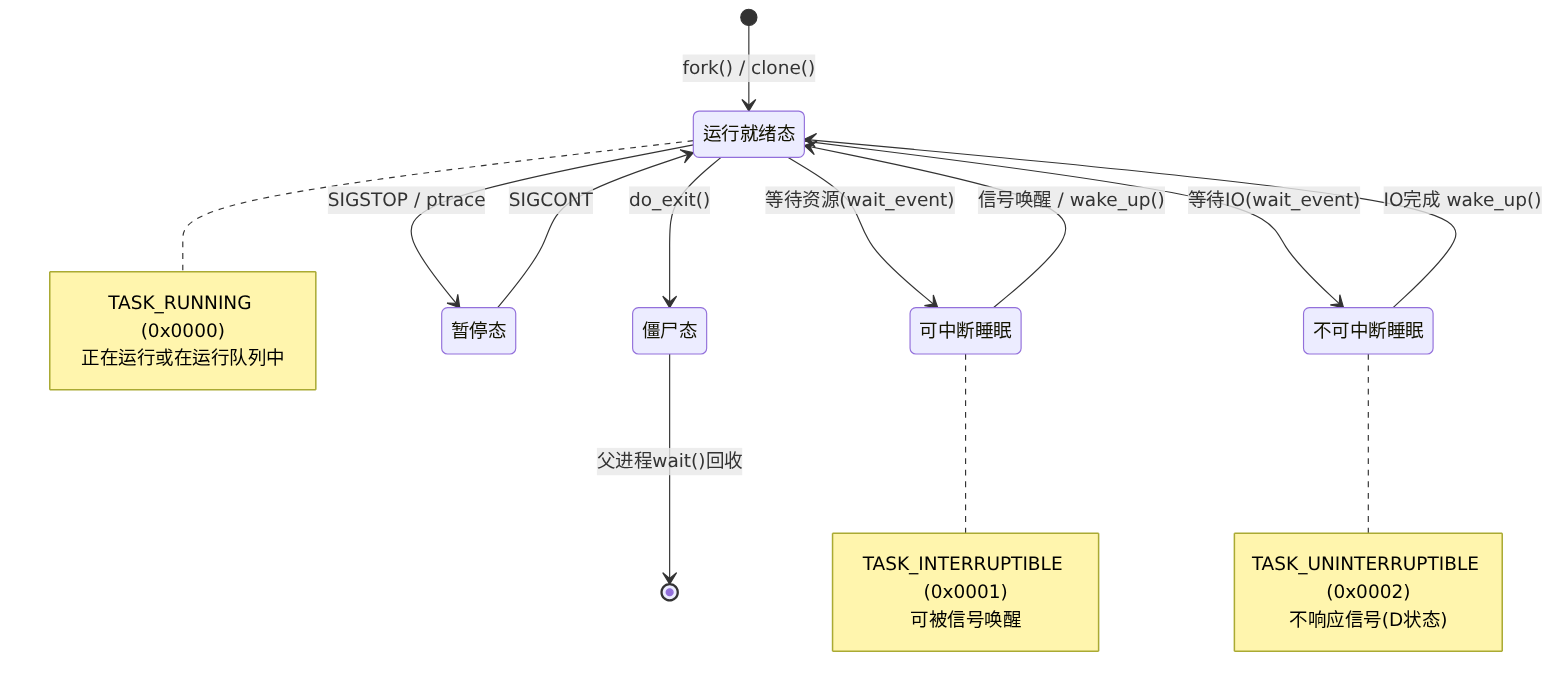
\includegraphics[width=0.85\textwidth]{fig_ch1_process_states.png}
\caption{Linux 进程状态机}
\label{fig_ch1_process_states}
\end{figure}

\subsection{进程创建 — fork / clone 调用链}

进程创建的唯一入口是 \texttt{kernel/fork.c} 中的 \texttt{kernel\_clone()}，它是 \texttt{fork()}, \texttt{vfork()}, \texttt{clone()} 三个系统调用的共同底层实现\cite{stevens}。

\begin{lstlisting}[language=C, caption={kernel\_clone 核心流程}, label={lst:fork}]
// kernel/fork.c
pid_t kernel_clone(struct kernel_clone_args *args) {
    // 1. 复制进程描述符——这是最核心的步骤
    p = copy_process(NULL, trace, NUMA_NO_NODE, args);
    // 2. 唤醒新进程加入调度队列
    wake_up_new_task(p);
    // 3. 返回子进程 PID
    return p->pid;
}
\end{lstlisting}

\texttt{copy\_process()}（\texttt{kernel/fork.c}）是进程创建的核心，调用链如下：

\textbf{步骤 1 — dup\_task\_struct()}：通过 \texttt{alloc\_task\_struct\_node()} 分配新的 \texttt{task\_struct} 和内核栈（通常为 \texttt{THREAD\_SIZE} = 16KB，包含 \texttt{thread\_info} 和内核栈），将父进程的 \texttt{task\_struct} 整体复制到子进程，然后清零子进程的特有字段（如 \texttt{pid}, \texttt{thread\_pid}）。

\textbf{步骤 2 — sched\_fork()}：初始化新进程的调度实体。将 \texttt{se.vruntime} 设置为父进程的 \texttt{vruntime}（保证公平性），设置 \texttt{se.on\_rq = 0}（尚未入队），初始化 \texttt{se.load} 权重为 \texttt{NICE\_0\_LOAD}（1024）。对于 EEVDF，还需初始化 \texttt{deadline}, \texttt{vlag} 等字段。

\textbf{步骤 3 — copy\_mm()}：根据 clone flags 决定共享还是复制地址空间。对于 \texttt{fork()}（非 \texttt{CLONE\_VM}），调用 \texttt{dup\_mm()} → \texttt{dup\_mmap()} 复制父进程的所有 VMA，同时将父子进程的页表项均标记为只读（COW 准备）。对于 \texttt{clone(CLONE\_VM)}（创建线程），直接共享 \texttt{mm\_struct}。

\textbf{步骤 4 — copy\_thread()}：架构相关初始化（\texttt{arch/x86/kernel/process\_64.c}）。设置 \texttt{thread.sp} 指向子进程内核栈上预留的 \texttt{pt\_regs} 区域底部，设置 \texttt{thread.ip} 为 \texttt{ret\_from\_fork} 汇编入口。

\textbf{步骤 5 — 唤醒}：\texttt{wake\_up\_new\_task()} → \texttt{activate\_task()} → \texttt{enqueue\_task()}，将子进程加入 CFS 红黑树，若子进程优先级高于当前进程则设置 \texttt{TIF\_NEED\_RESCHED} 标志。

\subsection{系统调用实现}

\subsubsection{系统调用注册}

在 Linux 6.x 中，添加系统调用仅需修改三个文件\cite{love}：

\begin{enumerate}[leftmargin=*]
    \item \texttt{arch/x86/entry/syscalls/syscall\_64.tbl}：注册系统调用号、ABI 类型、函数名。
    \item \texttt{kernel/sys.c} 或其他子系统文件：使用 \texttt{SYSCALL\_DEFINEn()} 宏实现系统调用函数体。
    \item \texttt{include/uapi/asm-generic/unistd.h}：更新 \texttt{\_\_NR\_syscalls} 的值。
\end{enumerate}

\subsubsection{系统调用入口 — entry\_SYSCALL\_64}

x86\_64 下系统调用通过 \texttt{syscall} 指令进入内核（\texttt{arch/x86/entry/entry\_64.S}）\cite{intel_sdm}，硬件自动将 RIP 保存到 RCX、RFLAGS 保存到 R11，从 IA32\_LSTAR MSR 加载内核入口 RIP（\texttt{entry\_SYSCALL\_64}），切换到 Ring 0 并使用内核栈。

\texttt{entry\_SYSCALL\_64} 汇编代码经过 \texttt{do\_syscall\_64()}（\texttt{arch/x86/entry/common.c}）根据 RAX 中的系统调用号查找 \texttt{sys\_call\_table} 数组，调用对应处理函数：

\begin{lstlisting}[language=C, caption={do\_syscall\_64 — 系统调用分发}, label={lst:do_syscall}]
// arch/x86/entry/common.c
__visible noinstr void do_syscall_64(struct pt_regs *regs, int nr) {
    if (likely(nr < NR_syscalls)) {
        regs->ax = sys_call_table[nr](regs);  // 返回结果写入 RAX
    }
}
\end{lstlisting}

\subsection{实验验证}

\subsubsection{实验2：系统调用添加}

本实验完成了向 Linux 6.18.15 内核添加自定义系统调用 \texttt{sys\_my\_add} 的全流程验证。内核侧修改三个文件：（1）\texttt{arch/x86/entry/syscalls/syscall\_64.tbl} 注册 \texttt{470 common my\_add sys\_my\_add}；（2）\texttt{kernel/sys.c} 中使用 \texttt{SYSCALL\_DEFINE2(my\_add, int a, int b)} 实现加法并添加参数合法性检查——负值输入返回 \texttt{-EINVAL}，同时输出 \texttt{printk(KERN\_INFO)} 内核日志；（3）\texttt{include/uapi/asm-generic/unistd.h} 将 \texttt{\_\_NR\_syscalls} 从 470 递增至 471。

编译采用增量方式（\texttt{make -j\$(nproc) bzImage}），验证方式为用户态程序通过 \texttt{syscall(\_\_NR\_my\_add, 10, 20)} 绕过 glibc 包装直接调用内核。返回值确认为 30（10+20），\texttt{dmesg} 输出 \texttt{"This is a new syscall: my\_add(10, 20) called"}。内核编译系统自动从 \texttt{.tbl} 文件生成 \texttt{unistd\_64.h}（含 \texttt{\_\_NR\_my\_add 470}）和 \texttt{syscalls\_64.h}（含 \texttt{\_\_SYSCALL(470, sys\_my\_add)}），验证了 Linux 6.x 系统调用表的自动生成机制。

该实验直接印证了 §1.4 所述的系统调用全路径：用户态 \texttt{syscall} 指令 → 硬件切换到 Ring 0 → \texttt{entry\_SYSCALL\_64} → \texttt{do\_syscall\_64()} 根据 RAX 索引 \texttt{sys\_call\_table[470]} → 调用 \texttt{\_\_x64\_sys\_my\_add()} → \texttt{sysretq} 返回用户态。

\subsubsection{实验3：哲学家进餐多线程实现}

本实验使用 POSIX 线程库实现了经典哲学家进餐问题的两个版本。死锁版本中五哲学家均遵循"先左叉后右叉"的对称策略，预防版本引入\textbf{偏序资源分配}：偶数号哲学家改为"先右叉后左叉"，从而打破循环等待环路。

线程同步通过 \texttt{pthread\_mutex\_t} 实现，五把互斥锁对应五把叉子。死锁检测由独立的观察者线程完成——该线程睡眠 5 秒后检查是否有哲学家仍处于 HUNGRY 状态且未达到预定进餐次数。测试采用自动化脚本连续运行 30 次预防版本，统计成功率。

实验结果：死锁版本在启动后数秒内稳定陷入死锁——所有五个哲学家均持有左叉等待右叉，形成完美的循环等待拓扑。预防版本 30 次运行全部成功（100\% 成功率），无一次死锁发生。该实验验证了 Coffman 死锁四条件中"循环等待"的破坏策略，从用户态层面印证了内核中 \texttt{futex} 系统调用对 \texttt{pthread\_mutex\_lock()} 的支撑——未竞争时通过原子操作在用户态完成加锁，竞争时才进入内核调用 \texttt{futex(FUTEX\_WAIT)} 进入睡眠。

%========================================== 第2章 ==========================================
\section{进程调度和x86架构下切换机制实现} \label{sec:ch2}

\textbf{本章为本报告重点章节，对 Linux 6.18.15 的进程调度核心逻辑与 x86\_64 架构下的上下文切换机制进行逐层深入的源码级分析。}

\subsection{调度器总体架构}

Linux 6.18.15 内核采用\textbf{调度类层次结构}（Scheduling Class Hierarchy）\cite{love,bovet,sched_cfs}，每个调度类实现一组标准的 \texttt{sched\_class} 回调接口。调度类按优先级从高到低排列如\tabref{tab:sched_classes}所示。

\begin{table}[htbp]
\centering
\caption{Linux 6.18.15 调度类层次}
\label{tab:sched_classes}
\begin{tabular}{lllP{5cm}}
\toprule
\textbf{优先级} & \textbf{调度类} & \textbf{策略} & \textbf{说明} \\
\midrule
0 (最高) & \texttt{stop\_sched\_class} & — & CPU 热插拔、任务迁移等内核关键操作 \\
1 & \texttt{dl\_sched\_class} & SCHED\_DEADLINE & 限期调度，基于 EDF+CBS 算法 \\
2 & \texttt{rt\_sched\_class} & SCHED\_FIFO / SCHED\_RR & 实时调度，优先级 1–99 \\
3 & \texttt{fair\_sched\_class} & SCHED\_NORMAL / BATCH & CFS/EEVDF 公平调度，优先级 100–139 \\
4 (最低) & \texttt{idle\_sched\_class} & SCHED\_IDLE & 每 CPU 的 idle 任务 \\
\bottomrule
\end{tabular}
\end{table}

调度类的链接顺序由 \texttt{include/asm-generic/vmlinux.lds.h} 中的链接脚本控制，保证遍历从最高优先级开始。\texttt{DEFINE\_SCHED\_CLASS} 宏（\texttt{kernel/sched/sched.h}）定义每个调度类实例，包含约 20 个回调函数指针：

\begin{lstlisting}[language=C, caption={sched\_class 核心回调（kernel/sched/sched.h）}, label={lst:sched_class}]
struct sched_class {
    unsigned int idx;
    void (*enqueue_task)(struct rq *rq, struct task_struct *p, int flags);
    void (*dequeue_task)(struct rq *rq, struct task_struct *p, int flags);
    void (*yield_task)(struct rq *rq);
    void (*wakeup_preempt)(struct rq *rq, struct task_struct *p, int flags);
    struct task_struct *(*pick_task)(struct rq *rq);
    struct task_struct *(*pick_next_task)(struct rq *rq);
    void (*put_prev_task)(struct rq *rq, struct task_struct *p);
    void (*set_next_task)(struct rq *rq, struct task_struct *p, bool first);
    void (*task_tick)(struct rq *rq, struct task_struct *p, int queued);
    void (*task_fork)(struct task_struct *p);
    void (*task_dead)(struct task_struct *p);
    void (*switched_from)(struct rq *rq, struct task_struct *p);
    void (*switched_to)(struct rq *rq, struct task_struct *p);
    void (*update_curr)(struct rq *rq);
};
\end{lstlisting}

\subsection{核心调度入口 — schedule() 与 \_\_schedule()}

\texttt{schedule()}（\texttt{kernel/sched/core.c}）在以下场景被调用\cite{lwn_context_switch}：进程主动调用 \texttt{sched\_yield()} 或 \texttt{schedule()}、等待资源时调用 \texttt{schedule\_timeout()} / \texttt{wait\_event()}、从中断/异常返回前检测到 \texttt{TIF\_NEED\_RESCHED} 标志。

\begin{lstlisting}[language=C, caption={schedule() 入口（kernel/sched/core.c）}, label={lst:schedule}]
void __sched schedule(void) {
    struct task_struct *tsk = current;
    sched_submit_work(tsk);
    __schedule(SM_NONE);
    sched_update_worker(tsk);
}
\end{lstlisting}

\texttt{\_\_schedule()} 是真正的调度决策函数，完成\textbf{选任务 → 切上下文}全流程。理解该函数的关键在于认识到：调用 \texttt{schedule()} 的进程将自己视为"prev"——它主动交出 CPU，期望调度器选择另一个进程（"next"）运行。

\textbf{分裂返回}是该函数最反直觉的语义。以下从 prev 和 next 两个视角展示一次完整的调度-切换-返回全时序：

\begin{table}[htbp]
\centering
\footnotesize
\caption{\_\_schedule() 分裂返回：prev 与 next 的双视角时序}
\label{tab:split_return}
\begin{tabular}{llP{5.5cm}P{4.5cm}}
\toprule
\textbf{步骤} & \textbf{执行者} & \textbf{prev 视角} & \textbf{next 视角} \\
\midrule
1 & prev & \texttt{schedule() → \_\_schedule()} 入口，prev 将自己设为当前任务 & next 此时可能在就绪队列中等待，或在某个等待队列中睡眠 \\
2 & prev & \texttt{pick\_next\_task()} 选中 next & （无感知）\\
3 & prev & \texttt{context\_switch()} 执行 \texttt{switch\_mm\_irqs\_off()} 切换地址空间 & （无感知）\\
4 & prev & \texttt{switch\_to(prev, next, prev)} → \texttt{\_\_switch\_to\_asm}：\texttt{push r15..rbp} 保存到 prev 内核栈，\texttt{mov \%rsp, prev->thread.sp} & （无感知）\\
$\blacktriangleright$ & \textbf{RSP切换点} & \texttt{mov next->thread.sp, \%rsp}：从此 RSP 指向 next 的内核栈 & \texttt{pop r15..rbp}：恢复上次自己被切出时的寄存器，\texttt{jmp \_\_switch\_to} \\
5 & next & prev 的指令流在此冻结，CPU 继续执行但"prev 不知道" & \texttt{\_\_switch\_to()} 收尾：更新 \texttt{current\_task}、切换 FPU/FSGSBASE、返回 prev 指针 \\
6 & next & （冻结中）& \texttt{context\_switch()} 返回 → \texttt{\_\_schedule()} 返回 → \texttt{schedule()} 返回。next 继续执行自己的业务逻辑 \\
7 & 将来的调度 & 某次调度器再次选中 prev，从 \texttt{prev->thread.sp} 恢复 RSP，\texttt{pop} 寄存器，\texttt{jmp \_\_switch\_to} → prev 从 \texttt{context\_switch} 返回 & （无感知）\\
8 & prev & prev 从 \texttt{\_\_schedule()} 返回，继续执行——它对步骤 5-7 之间发生的一切毫无记忆 & （可能已被切出）\\
\bottomrule
\end{tabular}
\end{table}

这张表揭示了一个关键事实：\textbf{prev 在 \texttt{\_\_switch\_to\_asm} 的 RSP 切换指令处被"冻结"，而 CPU 从此刻开始执行的是 next 的代码}。prev 内核栈上压着它的 callee-saved 寄存器，\texttt{prev->thread.sp} 指向那个位置。将来 prev 被再次调度时，\texttt{\_\_switch\_to\_asm} 后半段把寄存器全部弹回，\texttt{jmp \_\_switch\_to} 进入 C 函数，然后一路返回到 \texttt{context\_switch} → \texttt{\_\_schedule} → \texttt{schedule}。prev 对切换期间的所有事件（中断、其他进程的执行、时钟推进）完全无感知——它的"时间"在 RSP 切换点暂停，在恢复点继续。这就是为什么调度器代码中 \texttt{schedule()} 之后的代码不能假设任何有关"刚才发生了什么"的事情——你所在的 CPU 可能已经运行过数十个其他进程，你的 cache 行可能全部被逐出，你的 TLB 条目可能已被覆盖。这种"分裂返回"语义是理解整个调度器和上下文切换机制的核心。

\begin{lstlisting}[language=C, caption={\_\_schedule() 核心流程（kernel/sched/core.c）}, label={lst:__schedule}]
static void __sched notrace __schedule(int sched_mode) {
    struct task_struct *prev, *next;
    struct rq *rq;
    cpu = smp_processor_id();
    rq = cpu_rq(cpu);        // 获取当前CPU运行队列
    prev = rq->curr;         // 当前运行进程 = 即将变为 prev

    rq->donor = prev;
    SCHED_WARN_ON(current != prev);

    // ★ 核心：选择下一个要运行的任务
    pick_again:
    next = pick_next_task(rq, prev, &rf);
    if (next == prev) {
        rq->clock_update_flags &= ~(RQCF_ACT_SKIP|RQCF_REQ_SKIP);
        goto idle_exit;
    }

    // ★★★ 上下文切换：prev → next
    rq = context_switch(rq, prev, next, &rf);
    // 返回后，当前 CPU 已在 next 的上下文中执行
}
\end{lstlisting}

\subsection{pick\_next\_task() — 任务选择逻辑}

\begin{lstlisting}[language=C, caption={pick\_next\_task 与 \_\_pick\_next\_task（kernel/sched/core.c）}, label={lst:pick_next}]
static struct task_struct *
pick_next_task(struct rq *rq, struct task_struct *prev,
               struct rq_flags *rf) {
    // 快速路径：若所有就绪任务都是 CFS 普通进程
    if (likely(prev->sched_class == &fair_sched_class &&
               rq->nr_running == rq->cfs.h_nr_running)) {
        p = pick_next_task_fair(rq, prev, rf);
        if (unlikely(p == RETRY_TASK))
            goto restart;
        return p;
    }
    return __pick_next_task(rq, prev, rf);
}

static struct task_struct *
__pick_next_task(struct rq *rq, struct task_struct *prev,
                 struct rq_flags *rf) {
    // 遍历所有调度类：stop → dl → rt → fair → idle
    for_each_active_class(class) {
        p = class->pick_next_task(rq);
        if (p) return p;
    }
    BUG();  // idle 类应始终返回 idle 任务
}
\end{lstlisting}

\texttt{for\_each\_active\_class} 宏从最高优先级调度类（stop）开始遍历，调度类遍历顺序与\tabref{tab:sched_classes}一致\cite{sched_cfs}。

\subsection{CFS / EEVDF 公平调度分析}

\subsubsection{从 CFS 到 EEVDF 的演进}

Linux 6.18.15 的 CFS 调度器已从纯虚拟运行时间（vruntime）模型演进为\textbf{EEVDF（Earliest Eligible Virtual Deadline First）}算法\cite{sched_eevdf,lwn_eevdf,eevdf_paper}。关键差异如\tabref{tab:cfs_eevdf}所示。

\begin{table}[htbp]
\centering
\caption{CFS vs EEVDF 核心差异}
\label{tab:cfs_eevdf}
\begin{tabular}{lll}
\toprule
\textbf{维度} & \textbf{CFS (经典)} & \textbf{EEVDF (6.6+)} \\
\midrule
选择依据 & 最小 vruntime & 最小 virtual deadline \\
时间片分配 & 静态计算 & 动态 request\_size \\
延迟保证 & 近似 & 精确（有界延迟） \\
实体字段 & vruntime & deadline, min\_vruntime, vlag \\
\bottomrule
\end{tabular}
\end{table}

EEVDF 的核心思想：调度实体请求一段运行时间，调度器为其分配一个虚拟截止时间（virtual deadline），每次选择 deadline 最早且已 eligible 的实体运行。eligibility 通过比较实体的 \texttt{vlag} 和 \texttt{min\_vruntime} 动态判定。

\begin{lstlisting}[language=C, caption={sched\_entity — EEVDF 核心字段（include/linux/sched.h）}, label={lst:se_eevdf}]
struct sched_entity {
    struct load_weight    load;            // 负载权重
    struct rb_node        run_node;        // 红黑树节点
    unsigned int          on_rq;           // 是否在运行队列
    u64                   exec_start;      // 本次运行起始时间
    u64                   sum_exec_runtime;// 累计运行时间
    u64                   vruntime;        // 虚拟运行时间
    u64                   prev_sum_exec_runtime;
    u64                   deadline;        // ★ EEVDF: 虚拟截止时间
    u64                   min_vruntime;    // ★ EEVDF: 最小VRuntime边界
    u64                   vlag;            // ★ EEVDF: 滞后值（lag）
    struct sched_entity  *parent;
    struct cfs_rq        *cfs_rq;          // 所属 CFS 运行队列
};
\end{lstlisting}

\subsubsection{enqueue\_task\_fair / dequeue\_task\_fair — 入队出队}

\texttt{enqueue\_task\_fair()}（\texttt{kernel/sched/fair.c}）是任务加入调度队列的核心：

\begin{lstlisting}[language=C, caption={enqueue\_task\_fair 核心逻辑（kernel/sched/fair.c）}, label={lst:enqueue_fair}]
static void enqueue_task_fair(struct rq *rq, struct task_struct *p, int flags) {
    struct cfs_rq *cfs_rq = cfs_rq_of(&p->se);
    // 1. 若实体已在队列，直接返回（如 migration 场景）
    if (p->se.on_rq) return;
    // 2. 更新 vruntime（新唤醒的任务可能需补偿休眠时间）
    if (!(flags & ENQUEUE_WAKEUP) || (flags & ENQUEUE_MIGRATED))
        p->se.vruntime += cfs_rq->min_vruntime;
    // 3. 核心：插入 EEVDF 红黑树
    enqueue_entity(cfs_rq, &p->se, flags);
    // 4. 增加 nr_running 计数
    cfs_rq->h_nr_running++;
    // 5. 若新任务 deadline 早于当前任务，触发抢占
}
\end{lstlisting}

\texttt{enqueue\_entity()} 内部调用 \texttt{\_\_enqueue\_entity()} 将 \texttt{se->run\_node} 插入 \texttt{cfs\_rq->tasks\_timeline} 红黑树（按 deadline 排序），调用 \texttt{update\_min\_vruntime()} 更新 CFS 运行队列的最小虚拟运行时间，若新实体既不在运行中也不是当前实体，则调用 \texttt{update\_cfs\_group()} 更新组调度统计。

\texttt{dequeue\_task\_fair()} 执行反向操作：从红黑树中移除实体，递减 \texttt{nr\_running}，更新 \texttt{min\_vruntime}。

\subsubsection{pick\_task\_fair() → \_\_pick\_eevdf()}

CFS/EEVDF 的任务选择入口为 \texttt{pick\_task\_fair()}：

\begin{lstlisting}[language=C, caption={pick\_task\_fair（kernel/sched/fair.c）}, label={lst:pick_fair}]
static struct task_struct *pick_task_fair(struct rq *rq) {
    struct cfs_rq *cfs_rq = &rq->cfs;
    struct sched_entity *se;
    if (!cfs_rq->nr_queued) return NULL;
    // 调用 EEVDF 核心：选择最优调度实体
    se = pick_next_entity(rq, cfs_rq);
    return task_of(se);  // 从 sched_entity 反向获取 task_struct
}
\end{lstlisting}

\texttt{pick\_next\_entity()} 优先检查是否有预设的 \texttt{->next} 伙伴进程，否则调用 \texttt{\_\_pick\_eevdf()} 从红黑树中选择：

\begin{lstlisting}[language=C, caption={\_\_pick\_eevdf — EEVDF 核心选择（kernel/sched/fair.c）}, label={lst:eevdf}]
static struct sched_entity *__pick_eevdf(struct cfs_rq *cfs_rq) {
    struct rb_node *node = cfs_rq->tasks_timeline.rb_root.rb_node;
    struct sched_entity *best = NULL;
    while (node) {
        se = __node_2_se(node);
        // 检查实体是否满足 eligibility 条件
        if (entity_eligible(cfs_rq, se)) {
            best = se;
            node = node->rb_left;   // 在左子树找更小 deadline
        } else {
            node = node->rb_right;  // 不 eligible → 向右搜索
        }
    }
    return best;
}
\end{lstlisting}

\texttt{entity\_eligible()} 内部比较实体的 \texttt{vlag}：若 \texttt{vlag >= 0}，说明该实体尚未获得应得的 CPU 时间，具有 eligibility；若 \texttt{vlag < 0}，说明实体已超额运行，需等待其他实体追赶。

\textbf{为什么 EEVDF 需要 eligibility 检查——CFS 的"唤醒风暴"问题。}经典 CFS 按最小 vruntime 选进程。考虑一个场景：100 个进程每 10ms 做一次 \texttt{read()} 等待磁盘 I/O，还有一个纯 CPU 计算的进程在后台。每次 I/O 完成，唤醒的进程 vruntime 极小（它睡了很久，vruntime 没增长），于是 \texttt{pick\_next\_task\_fair} 立刻选它、抢占当前 CPU 进程。100 个进程 × 每秒 100 次唤醒 = 每秒 100 次上下文切换，CPU 的大量时间消耗在切换本身而非实际计算。EEVDF 用 eligibility 解决了这个问题：刚被唤醒的进程虽然在就绪队列中，但它的 vlag 为负——它睡觉期间没有"消费"CPU，但从系统的角度看，它"欠"了其他一直在就绪的进程。只有等 vlag 归零（其他进程追赶上它的 vruntime），该进程才算 eligible，才能被 \texttt{pick\_next\_entity} 选中。这本质上是把调度决策从"谁最缺 CPU"变为"谁既不缺 CPU、deadline 又最近"\cite{sched_eevdf,lwn_eevdf}。

\subsubsection{时钟中断与抢占检查 — scheduler\_tick()}

每次时钟中断触发 \texttt{scheduler\_tick()}，调用链为 \texttt{scheduler\_tick() → task\_tick\_fair() → entity\_tick()}：

\begin{lstlisting}[language=C, caption={entity\_tick 时间片更新与抢占检查（kernel/sched/fair.c）}, label={lst:entity_tick}]
static void entity_tick(struct cfs_rq *cfs_rq, struct sched_entity *curr) {
    // 1. 更新当前实体的 vruntime 和 deadline 统计
    update_curr(cfs_rq);
    // 2. 若运行队列中不止一个任务，检查是否需要抢占
    if (cfs_rq->nr_running > 1)
        check_preempt_tick(cfs_rq, curr);
}
\end{lstlisting}

\texttt{update\_curr()} 计算当前实体的实际运行时间增量（\texttt{delta\_exec = now - exec\_start}），按负载权重缩放后累加到 \texttt{vruntime}，同时更新 \texttt{min\_vruntime}。\texttt{check\_preempt\_tick()} 比较当前实体与红黑树中最左实体的 deadline，若当前实体的剩余时间片已耗尽或最左实体的 deadline 显著更早，设置 \texttt{TIF\_NEED\_RESCHED} 标志。

\textbf{唤醒抢占}：\texttt{try\_to\_wake\_up() → check\_preempt\_curr() → check\_preempt\_wakeup()}。若被唤醒进程的 deadline 早于当前进程的 deadline 且满足 eligibility 条件，调用 \texttt{resched\_curr()} 设置抢占标志。

\subsection{上下文切换：context\_switch()}

\texttt{context\_switch()}（\texttt{kernel/sched/core.c}）是进程切换的中央调度函数，完成了从 prev 进程到 next 进程的完整状态转移。该函数分两个半场：

\begin{lstlisting}[language=C, caption={context\_switch 核心结构（kernel/sched/core.c）}, label={lst:context_switch}]
static __always_inline struct rq *
context_switch(struct rq *rq, struct task_struct *prev,
               struct task_struct *next, struct rq_flags *rf) {
    prepare_task_switch(rq, prev, next);      // 准备阶段

    // ★ 上半场：地址空间切换
    arch_start_context_switch(prev);
    switch_mm_irqs_off(prev->active_mm, next->mm, next);

    // ★ 下半场：执行现场切换
    switch_to(prev, next, prev);
    // ↑ 第三个参数 prev 在返回后变为 last（从哪个进程切换来）
    return finish_task_switch(prev);
}
\end{lstlisting}

\subsubsection{地址空间切换 — switch\_mm\_irqs\_off()}

\texttt{switch\_mm\_irqs\_off()}（\texttt{arch/x86/mm/tlb.c}）完成虚拟地址空间的切换\cite{lwn_context_switch}：

\begin{lstlisting}[language=C, caption={switch\_mm\_irqs\_off — CR3 切换（arch/x86/mm/tlb.c）}, label={lst:switch_mm}]
void switch_mm_irqs_off(struct mm_struct *prev, struct mm_struct *next,
                        struct task_struct *tsk) {
    if (prev == next) return;           // 内核线程，无需切换
    // 选择新 ASID（Address Space Identifier，PCID 特性）
    choose_new_asid(next, next_tlb_gen, &new_asid, &need_flush);
    // ★ 加载新页表基址到 CR3 寄存器
    load_new_mm_cr3(next->pgd, new_asid, need_flush);
    this_cpu_write(cpu_tlbstate.loaded_mm, next);
}
\end{lstlisting}

\texttt{load\_new\_mm\_cr3()} 通过 \texttt{write\_cr3()} 内联汇编写入 CR3 寄存器。现代 x86 处理器支持 PCID（Process-Context Identifier），允许 TLB 条目携带地址空间标签，避免每次 CR3 写入时全量刷新 TLB。\texttt{choose\_new\_asid()} 函数负责分配新的 ASID 并决定是否需要 TLB 刷新\cite{intel_sdm}。

\textbf{PCID 的一个常见误解需要澄清}：PCID 不是"让上下文切换不刷新 TLB"——它的实际效果更微妙。没有 PCID 时，写入 CR3 刷新\textbf{全部} TLB 条目，包括内核空间那些标记为 Global 的条目（它们本该对所有进程有效）。有了 PCID，每个进程拥有独立的 ASID（Address Space Identifier），其 TLB 条目仅在 ASID 匹配时命中。这意味着：① 切换到新进程时不必显式刷新 TLB——旧 ASID 的条目自然不会被新 ASID 的访问匹配到；② 内核空间的 Global 条目在 CR3 写入后仍然存活——这些条目对性能至关重要（内核代码路径、中断处理、系统调用入口）；③ 当切换回一个刚离开不久的进程时，其 TLB 条目可能仍在（取决于 TLB 容量），可实现部分复用。PCID 的真正价值是"让无关进程的 TLB 条目在硬件中和平共存"，而非单纯"免刷新"\cite{intel_sdm}。

\subsubsection{执行现场切换 — switch\_to 宏 → \_\_switch\_to\_asm}

\texttt{switch\_to}（\texttt{arch/x86/include/asm/switch\_to.h}）是执行流切换的核心宏：

\begin{lstlisting}[language=C, caption={switch\_to 宏定义（arch/x86/include/asm/switch\_to.h）}, label={lst:switch_to}]
#define switch_to(prev, next, last)                    \
do {                                                   \
    ((last) = __switch_to_asm((prev), (next)));        \
} while (0)
\end{lstlisting}

\texttt{\_\_switch\_to\_asm()}（\texttt{arch/x86/entry/entry\_64.S}）是上下文切换最底层的汇编实现，执行以下五个步骤\cite{x86_abi}：

\begin{lstlisting}[caption={\_\_switch\_to\_asm 汇编实现（arch/x86/entry/entry\_64.S）}, label={lst:switch_asm}]
SYM_FUNC_START(__switch_to_asm)
    /* %rdi = prev, %rsi = next */

    /* 1. Save callee-saved registers onto prev's stack */
    pushq   %rbp
    pushq   %rbx
    pushq   %r12
    pushq   %r13
    pushq   %r14
    pushq   %r15

    /* 2. Save prev's RSP -> prev->thread.sp */
    movq    %rsp, TASK_threadsp(%rdi)

    /* 3. Load next's RSP <- next->thread.sp */
    movq    TASK_threadsp(%rsi), %rsp

    /* ★ EXECUTION FLOW NOW RUNS ON next's KERNEL STACK ★ */

    /* 4. Restore next's callee-saved registers */
    popq    %r15
    popq    %r14
    popq    %r13
    popq    %r12
    popq    %rbx
    popq    %rbp

    /* 5. Jump to __switch_to() C function */
    jmp     __switch_to
SYM_FUNC_END(__switch_to_asm)
\end{lstlisting}

\subsubsection{\_\_switch\_to\_asm 寄存器状态逐帧分析}

\textbf{帧 0 — 进入}：RDI = prev \texttt{task\_struct *}，RSI = next \texttt{task\_struct *}，RSP = prev 的内核栈顶，RIP = \texttt{\_\_switch\_to\_asm} 第一条指令。

\textbf{帧 1–6 — 保存 prev 现场}：依次 \texttt{pushq \%rbp, \%rbx, \%r12, \%r13, \%r14, \%r15}，六次 push 后 RSP 下降 48 字节，prev 内核栈顶存储完整 \texttt{inactive\_task\_frame} 结构。该结构保证压栈/弹栈次序严格匹配，是 \texttt{\_\_switch\_to\_asm} 正确性的关键。

\textbf{帧 7 — RSP 切换点}：\texttt{movq \%rsp, TASK\_threadsp(\%rdi)} 将当前 RSP 写入 \texttt{prev->thread.sp}。\texttt{movq TASK\_threadsp(\%rsi), \%rsp} 将 RSP 替换为 \texttt{next->thread.sp}。\textbf{此时 RSP 指向 next 的内核栈——执行流已切换。}

\textbf{帧 8–13 — 恢复 next 现场}：逆序弹出 \texttt{\%r15, \%r14, \%r13, \%r12, \%rbx, \%rbp}，恢复 next 上次被切换出时的全部 callee-saved 寄存器值。

\textbf{帧 14 — 架构收尾}：\texttt{jmp \_\_switch\_to} 进入 C 函数。\texttt{\_\_switch\_to()}（\texttt{arch/x86/kernel/process\_64.c}）是上下文切换的 C 语言收尾阶段，其核心职责是将 CPU 的"管理结构"从 prev 切换到 next，而非寄存器现场（寄存器现场已在 \texttt{\_\_switch\_to\_asm} 中完成切换）：

\begin{lstlisting}[language=C, caption={\_\_switch\_to C 语言收尾（arch/x86/kernel/process\_64.c）}, label={lst:__switch_to_c}]
struct task_struct *__switch_to(struct task_struct *prev,
                                struct task_struct *next) {
    // 1. 更新 per-CPU 的 current_task 为 next
    this_cpu_write(current_task, next);

    // 2. 切换 FPU/SIMD 状态（XSAVE 指令保存/恢复）
    //    — 若 prev 使用了 AVX/AMX，保存其寄存器上下文
    //    — 若 next 之前被切换出时 FPU 状态未脏，则跳过恢复
    switch_fpu(prev, next);

    // 3. 切换 FS/GS 段寄存器（线程局部存储 TLS）
    x86_fsgsbase_load(prev, next);

    // 4. 扩展状态切换：DEBUG 寄存器、I/O 权限位图
    //    perf 事件上下文等非通用寄存器状态
    __switch_to_xtra(prev, next);

    return prev;  // 返回 prev（即 switch_to 宏中的 last）
}
\end{lstlisting}

\texttt{switch\_fpu()} 是其中的性能关键点。现代处理器（支持 XSAVE/AVX/AMX）的 FPU 状态可达数 KB，每次上下文切换都完整保存和恢复将带来显著开销。Linux 通过\textbf{惰性 FPU 切换}优化：\texttt{switch\_fpu()} 仅将 prev 的 FPU 状态标记为"脏"（若其实际使用过 FPU），而不立即保存；只有当下一次调度选择使用 FPU 的其他进程时，才通过 \texttt{xsave} 指令保存 prev 的 FPU 状态到 \texttt{prev->thread.fpu}，并通过 \texttt{xrstor} 恢复 next 的状态。若 prev 从未使用过 FPU（如纯整数计算进程），整个保存步骤被省略\cite{amd_apm}。

\textbf{上下文切换的真实成本。}表面上看，\texttt{\_\_switch\_to\_asm} 只做了 6 个 push + RSP 切换 + 6 个 pop + 1 个 jmp，约 20 条指令、几十个 cycle。但这只是冰山浮尖。真正的开销在切换之后：

\begin{itemize}[leftmargin=*]
    \item \textbf{TLB 失效}：CR3 写入后，若无 PCID，整个 TLB 被刷新。新进程的每次内存访问都是 TLB miss——页表遍历需要 4 次内存访问（pgd→p4d→pud→pmd→pte，五级页表），每次约 10–20 cycles。进程恢复执行后的前几十次访存几乎全部 TLB miss。
    \item \textbf{Cache 污染}：L1/L2/L3 cache 中填满了 prev 的数据。next 的代码和数据首次访问几乎必定 cache miss——L2 miss 约 40 cycles，L3 miss 约 200 cycles，DRAM 访问约 200ns。
    \item \textbf{分支预测器状态错位}：现代 CPU 的分支预测器使用全局历史（过去若干分支的 taken/not-taken 模式）做预测。切换到 next 后，分支预测器看到的是 prev 的历史、执行的是 next 的代码——前几十个分支几乎随机预测，平均 2–3 次误预测（每次约 20 cycles 的流水线冲刷）。
    \item \textbf{综合估算}：一次完整的上下文切换（含 CR3 写入），在无 PCID 的 x86\_64 处理器上，真实开销在 \textbf{3,000–10,000 cycles}。其中 \texttt{\_\_switch\_to\_asm} 的指令执行本身占比不到 1\%。引入 PCID 后 TLB 刷新被避免，但 cache 污染和分支预测器偏移仍然存在\cite{intel_sdm}。
\end{itemize}

上下文切换的完整调用时序如\figref{fig_ch2_switch_to_asm}所示。

\begin{figure}[htbp]
\centering
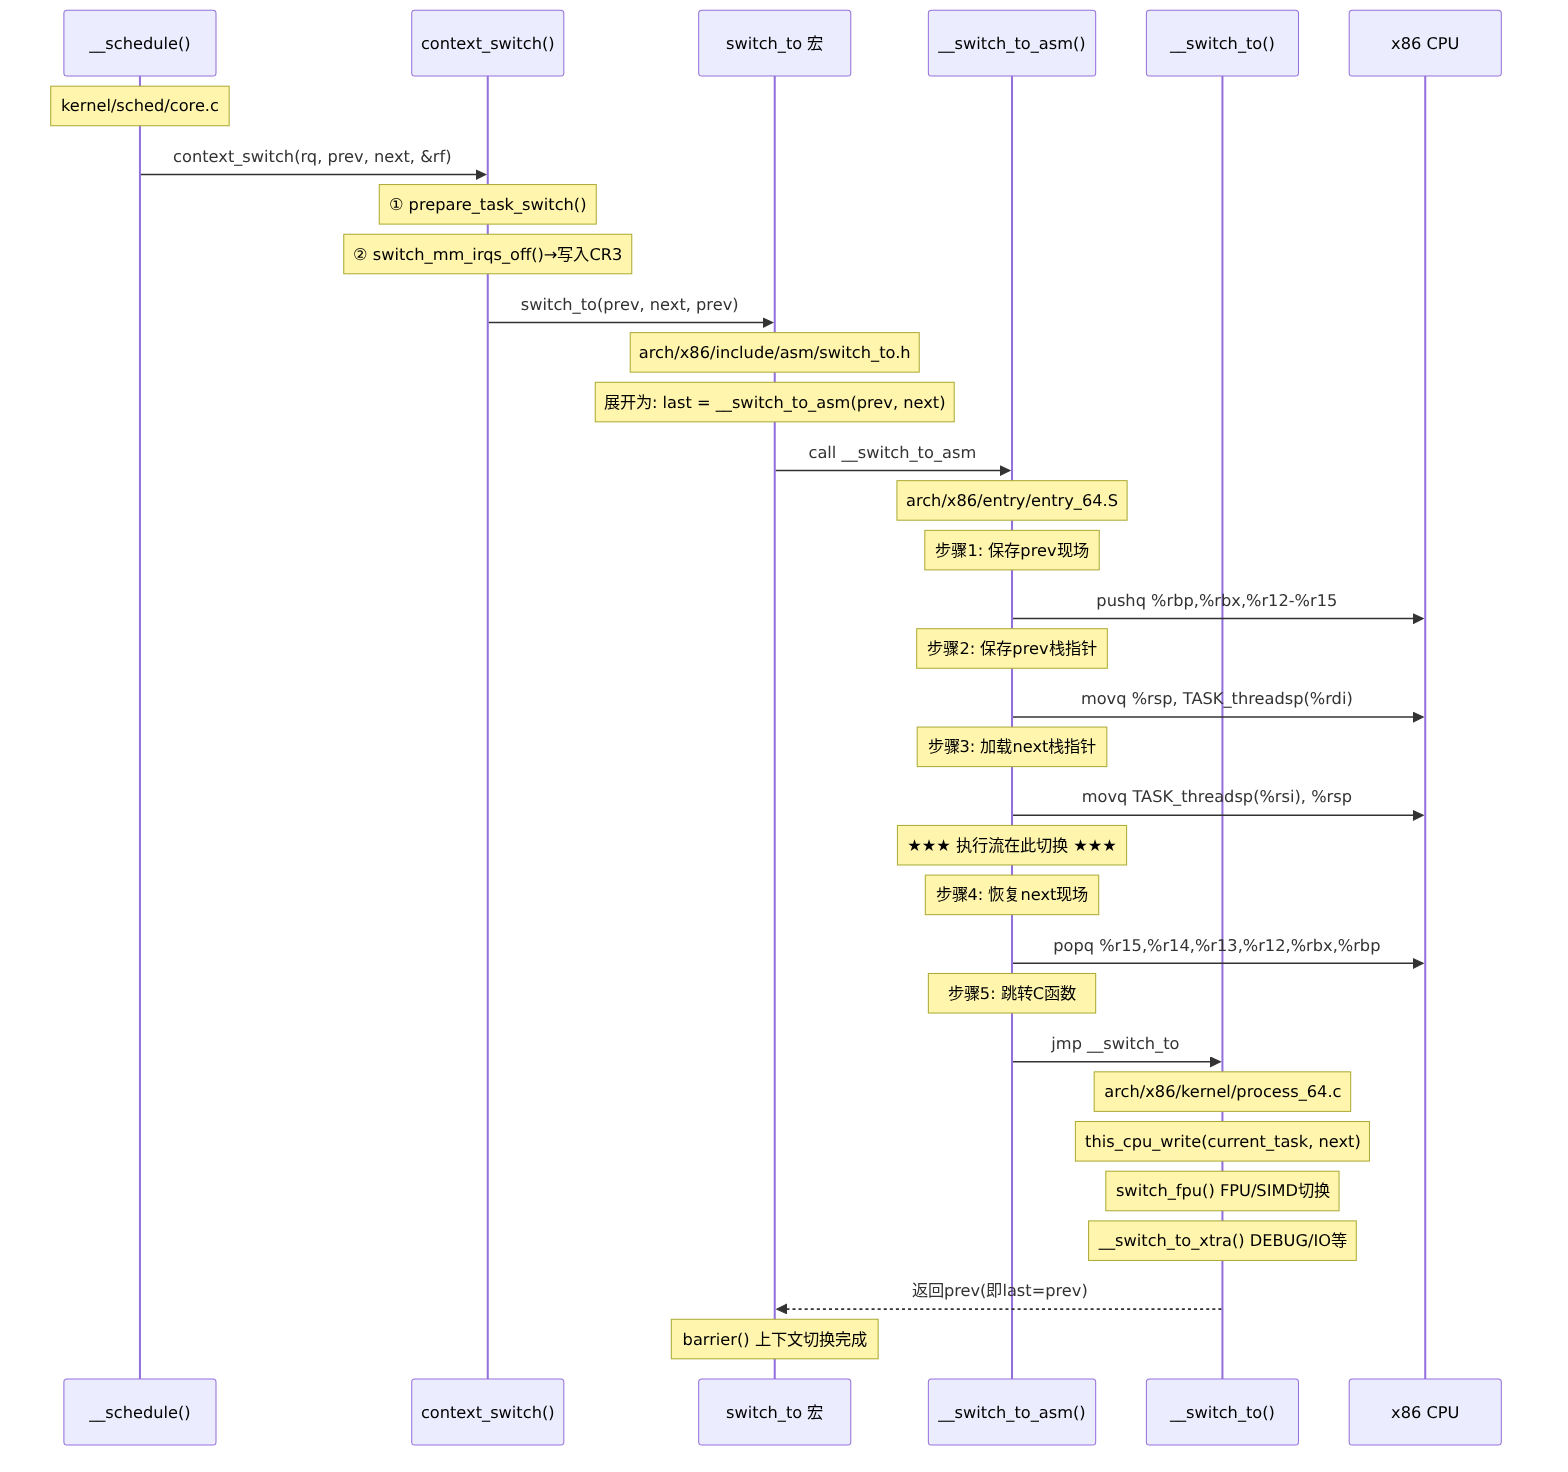
\includegraphics[width=0.95\textwidth,height=0.88\textheight,keepaspectratio]{fig_ch2_switch_to_asm.png}
\caption{\_\_switch\_to\_asm 寄存器级切换时序}
\label{fig_ch2_switch_to_asm}
\end{figure}

\subsection{完整调度调用链}

从 \texttt{schedule()} 到 \texttt{\_\_switch\_to()} 的完整调用链如\figref{fig_ch2_schedule_call_chain}所示。

\begin{figure}[htbp]
\centering
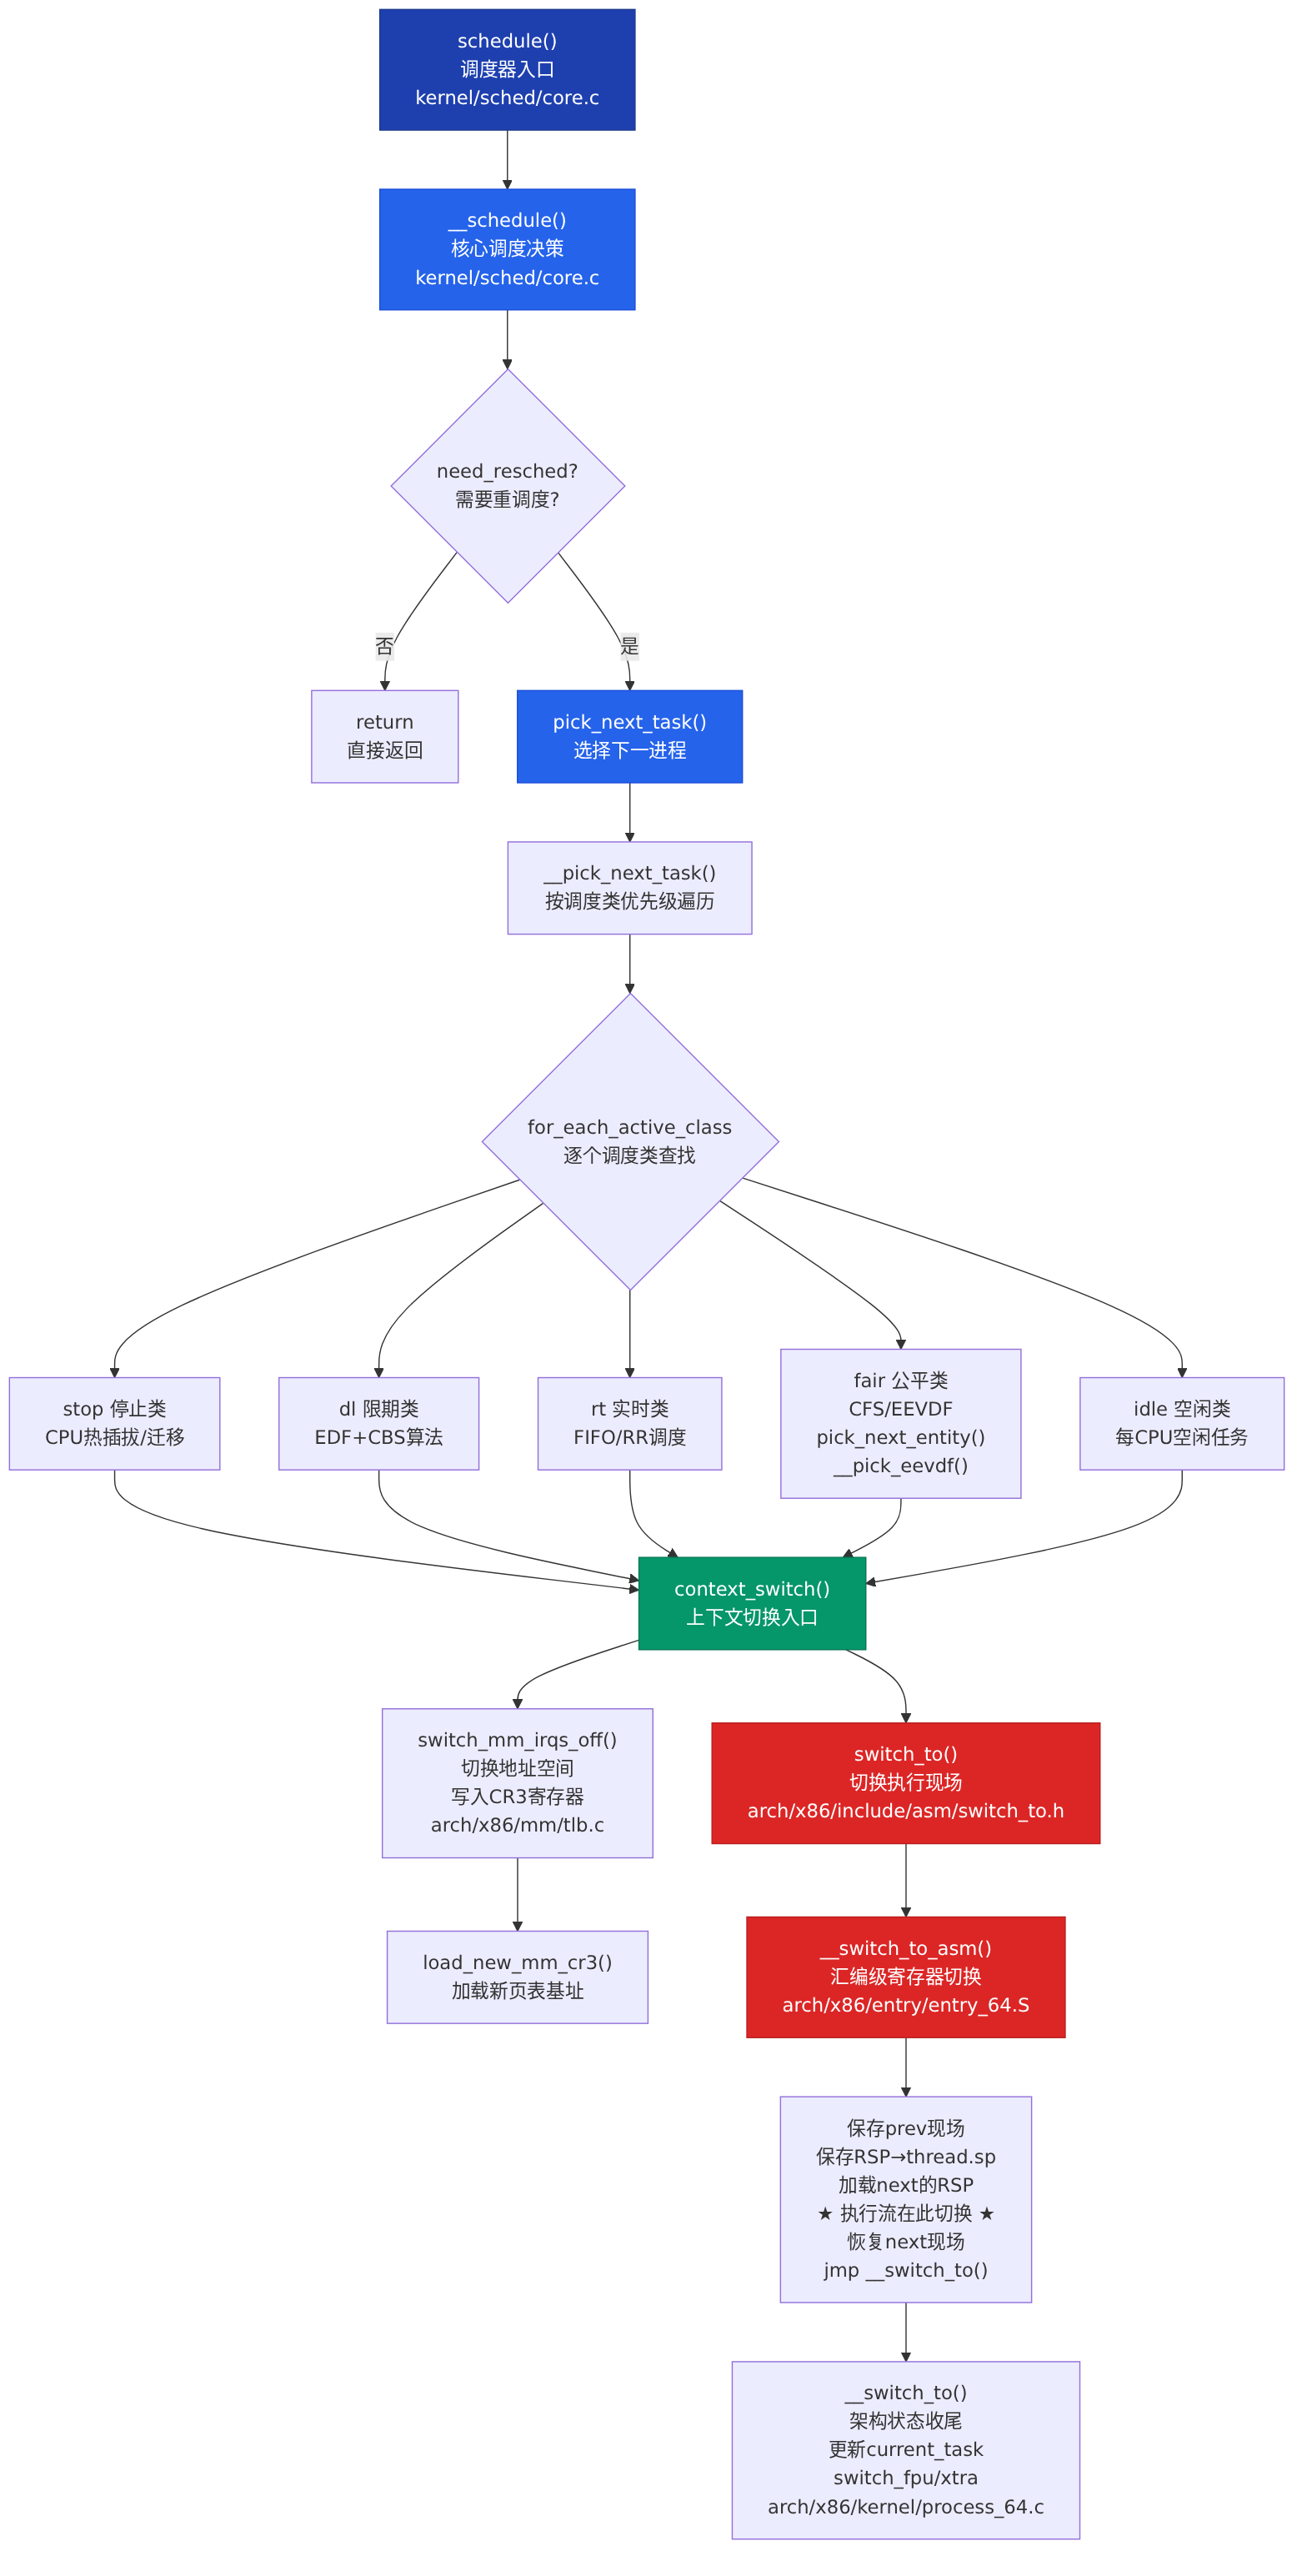
\includegraphics[width=0.95\textwidth,height=0.88\textheight,keepaspectratio]{fig_ch2_schedule_call_chain.png}
\caption{schedule() → \_\_schedule() → context\_switch() 完整调用链}
\label{fig_ch2_schedule_call_chain}
\end{figure}

\subsection{结构体关系}

\figref{fig_ch2_task_struct} 展示了 \texttt{task\_struct}, \texttt{sched\_entity}, \texttt{cfs\_rq}, \texttt{rq}, \texttt{thread\_struct} 之间的包含与引用关系。\figref{fig_ch2_sched_classes} 展示了调度类层次结构的遍历顺序。

\begin{figure}[htbp]
\centering
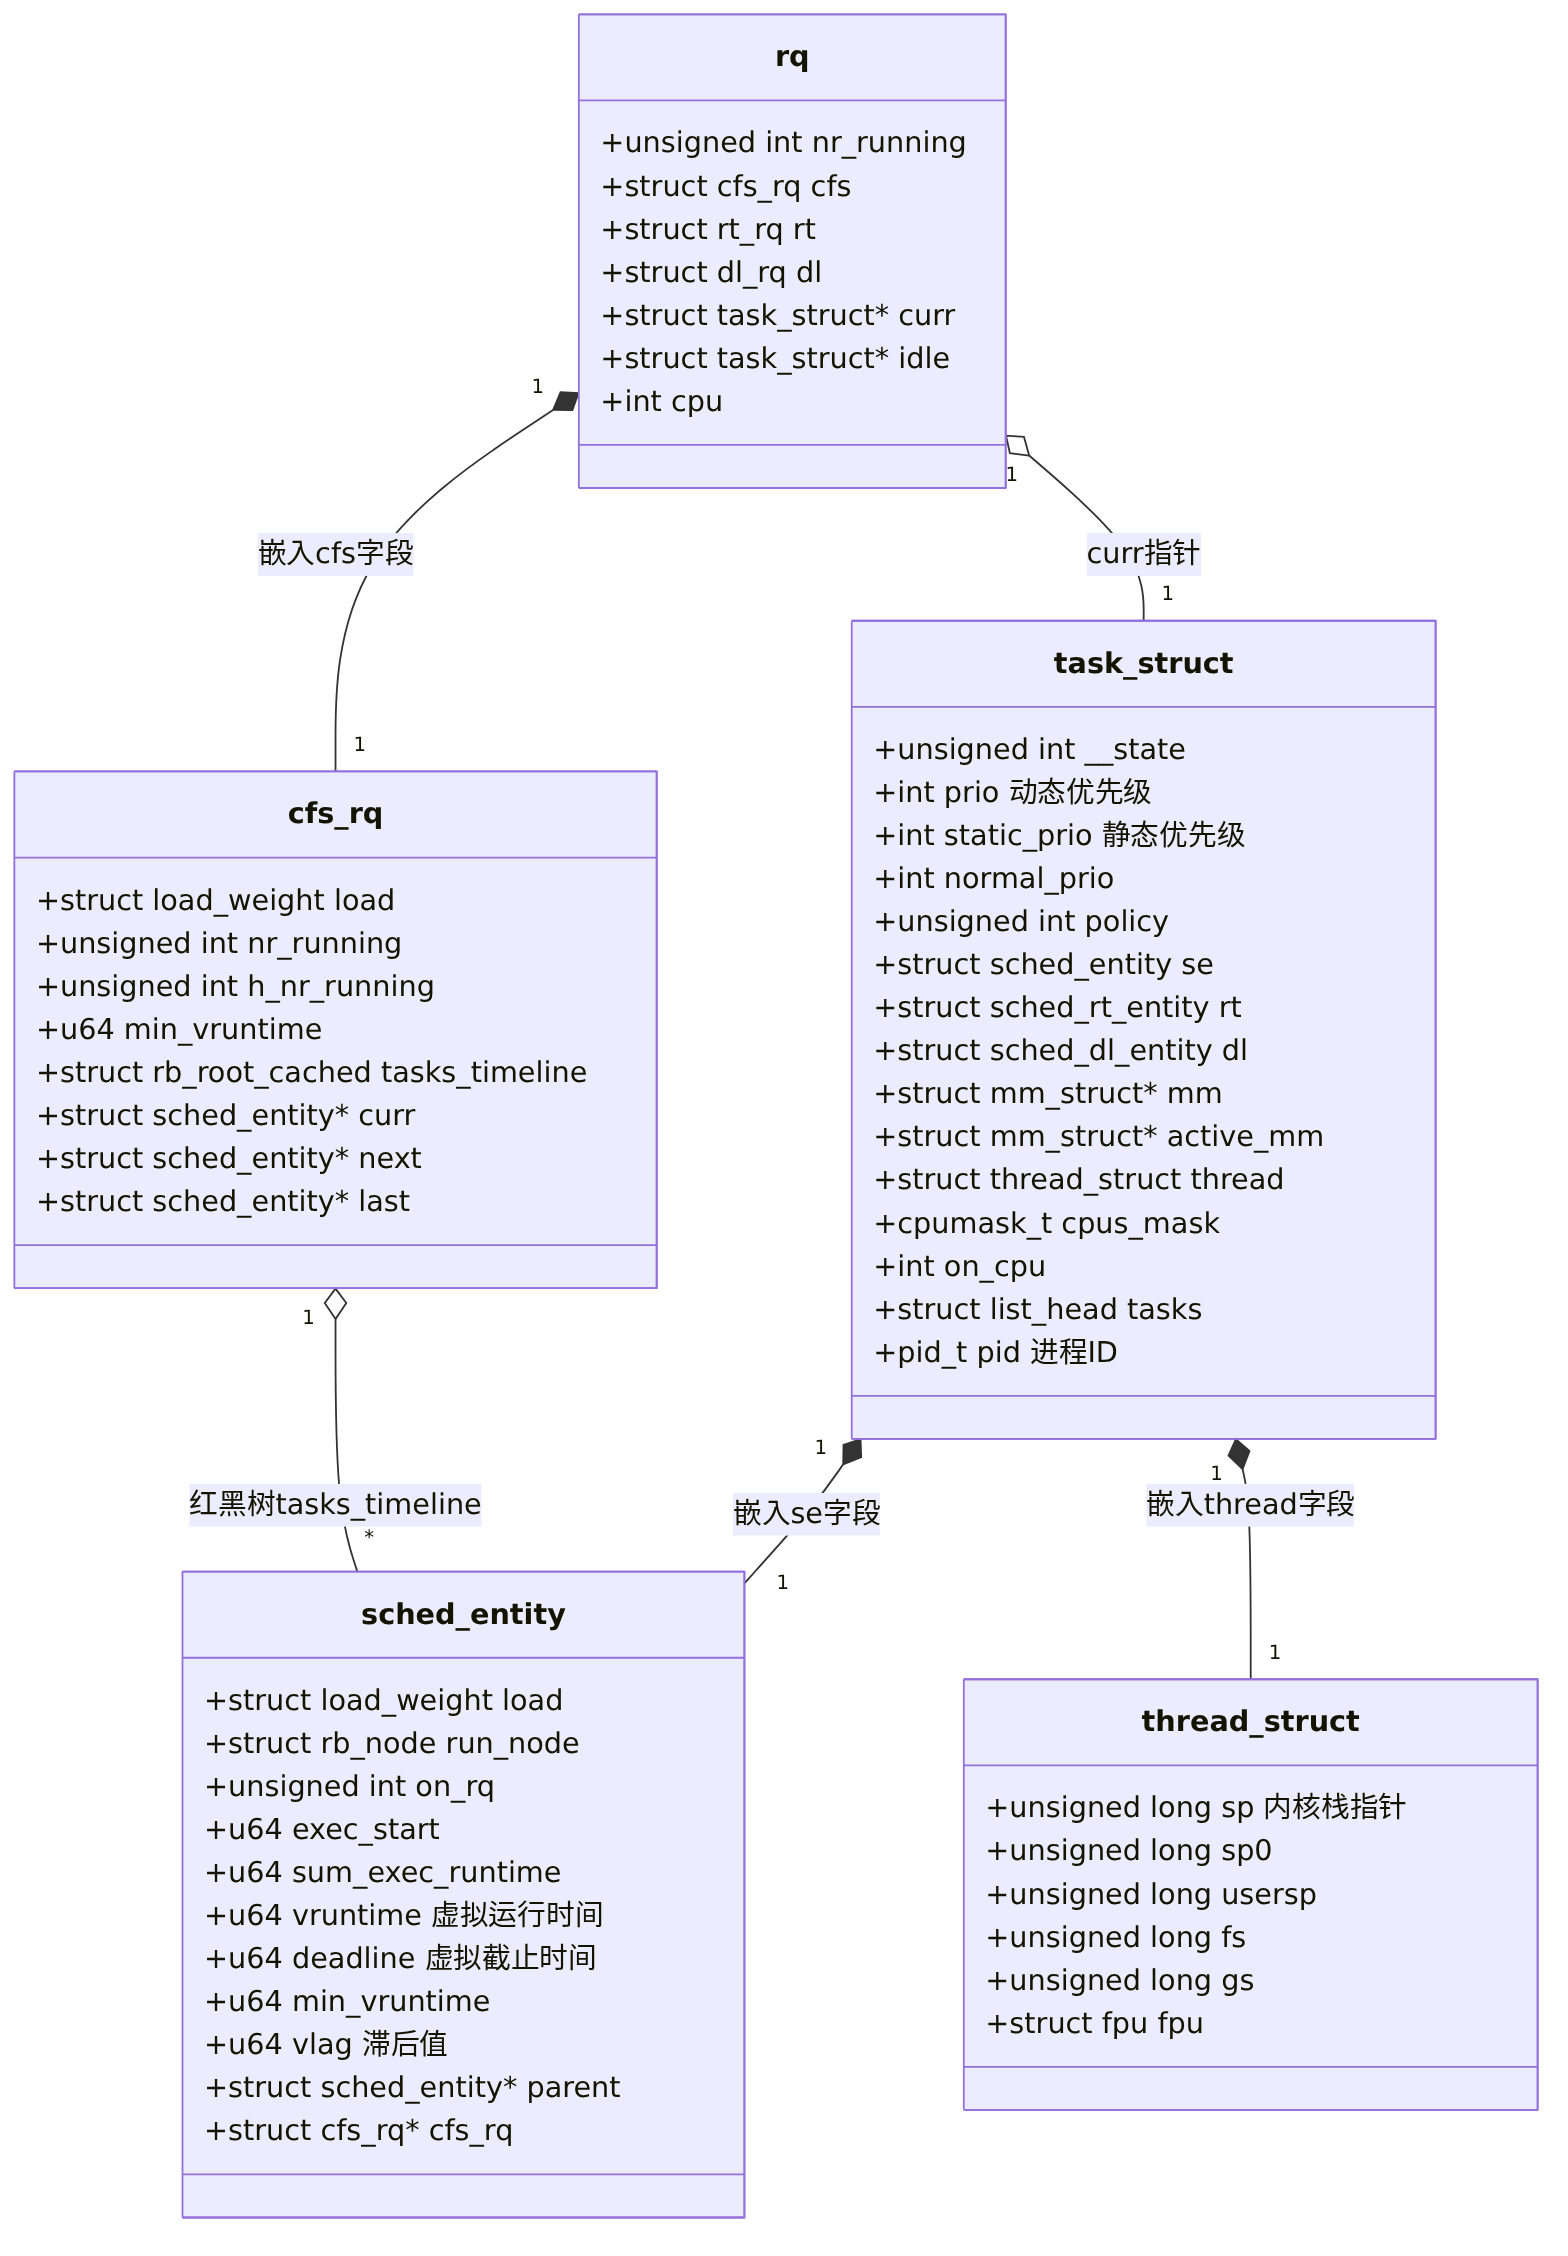
\includegraphics[width=0.95\textwidth,height=0.88\textheight,keepaspectratio]{fig_ch2_task_struct.png}
\caption{task\_struct / sched\_entity / cfs\_rq / rq 结构体关系}
\label{fig_ch2_task_struct}
\end{figure}

\begin{figure}[htbp]
\centering
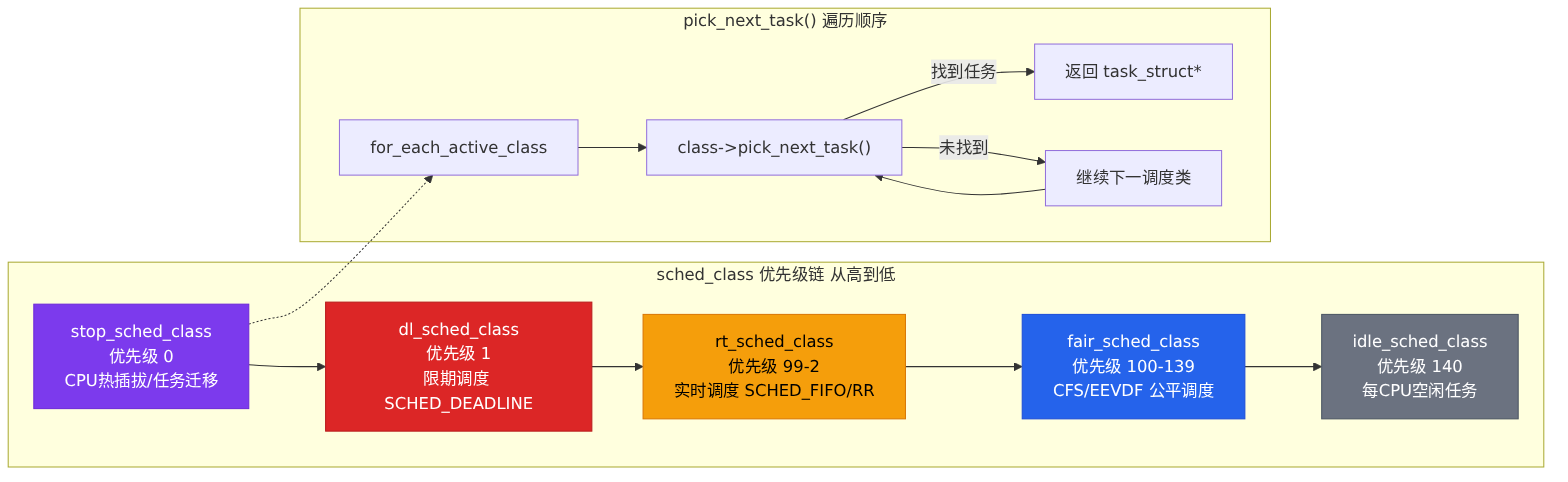
\includegraphics[width=0.9\textwidth]{fig_ch2_sched_classes.png}
\caption{调度类优先级层次与 pick\_next\_task 遍历顺序}
\label{fig_ch2_sched_classes}
\end{figure}

\subsection{调度类实战：SCHED\_MFQ 完整实现分析}

前文从通用架构层面分析了 Linux 调度器的层次结构和调用链。本节以实验 11 中实际实现的 \texttt{SCHED\_MFQ}（Multi-level Feedback Queue，多级反馈队列，policy=4）调度类为完整案例，展示如何从零开始实现一个新的调度类并将其集成到 Linux 6.18.15 内核中。该案例覆盖了调度类注册、数据结构嵌入、全部回调函数实现、内核编译集成以及用户态调用验证的完整链路，是对前文所有调度理论分析的工程验证。

\subsubsection{MFQ 算法设计}

MFQ 由 Fernando J. Corbató 于 1962 年在 CTSS 系统中首次提出\cite{mfq_paper}。本实现采用 8 级队列（L0–L7），每级时间片为 \texttt{10 << level} ticks：

\begin{table}[htbp]
\centering
\caption{SCHED\_MFQ 队列参数}
\label{tab:mfq_params}
\begin{tabular}{cccc}
\toprule
\textbf{队列} & \textbf{时间片 (ticks)} & \textbf{目标进程类型} \\
\midrule
L0（最高优先级）& 10 & 新进程、I/O 密集型 \\
L1 & 20 & 轻度 CPU 密集型 \\
L2 & 40 & — \\
L3 & 80 & — \\
L4 & 160 & — \\
L5 & 320 & — \\
L6 & 640 & — \\
L7（最低优先级）& 1280 & 纯 CPU 密集型后台任务 \\
\bottomrule
\end{tabular}
\end{table}

核心规则：
\begin{enumerate}[leftmargin=*]
    \item 新进程进入 L0（最高优先级）。
    \item 时间片耗尽且队列中有其他进程 → 降级（level++），时间片翻倍。
    \item 队列中唯一进程 → 不降级（降级无意义）。
    \item I/O 同步唤醒（\texttt{WF\_SYNC} 标志）→ 升级（level--），并可能抢占当前进程。
\end{enumerate}

\subsubsection{内核数据结构嵌入}

实现新调度类的第一步是在内核核心数据结构中嵌入调度器私有字段。需要修改三个文件：

\textbf{include/linux/sched.h} —— 在 \texttt{task\_struct} 中嵌入 \texttt{sched\_mfq\_entity}：

\begin{lstlisting}[language=C, caption={task\_struct 中的 MFQ 实体嵌入（include/linux/sched.h）}, label={lst:mfq_task_struct}]
// include/linux/sched.h, line ~880
struct task_struct {
    // ... 其他字段 ...
    struct sched_entity     se;          // CFS 调度实体
#ifdef CONFIG_SCHED_MFQ
    struct sched_mfq_entity mfq_se;      // ★ MFQ 调度实体(新增)
#endif
    struct sched_rt_entity  rt;          // RT 调度实体
    // ...
};

// 同时需要定义 sched_mfq_entity 结构体：
struct sched_mfq_entity {
    struct list_head    run_list;        // 链接到 mfq_rq.queues[level]
    int                 queue_level;     // 当前队列级别 (0-7)
    u64                 time_slice;      // 剩余时间片 (ticks)
};
\end{lstlisting}

\textbf{kernel/sched/sched.h} —— 定义 per-CPU 的 MFQ 运行队列和调度类声明：

\begin{lstlisting}[language=C, caption={mfq\_rq 结构和调度类声明（kernel/sched/sched.h）}, label={lst:mfq_rq}]
// kernel/sched/sched.h
#define MFQ_QUEUE_LEVELS 8

struct mfq_rq {
    raw_spinlock_t      lock;            // 保护本 MFQ 队列的锁
    unsigned int        nr_running;      // 当前在队列中的任务数
    struct list_head    queues[MFQ_QUEUE_LEVELS]; // 8级就绪队列
    struct task_struct *curr;            // 当前在此CPU运行的MFQ任务
};

DECLARE_PER_CPU(struct mfq_rq, mfq_rq);  // per-CPU 变量声明
extern const struct sched_class mfq_sched_class; // 调度类外部声明
\end{lstlisting}

\textbf{include/uapi/linux/sched.h} —— 注册调度策略常量：

\begin{lstlisting}[language=C, caption={SCHED\_MFQ 策略注册（include/uapi/linux/sched.h）}, label={lst:mfq_policy}]
#define SCHED_MFQ    4    // MFQ 调度策略号（新增）
\end{lstlisting}

\subsubsection{调度类注册与集成}

新调度类需要在内核的三个关键位置注册，使其参与调度决策：

\textbf{① 调度类路由（kernel/sched/core.c）}：在 \texttt{\_\_setscheduler\_class()} 中添加 MFQ 分支，使 \texttt{sched\_setscheduler()} 系统调用能将任务的调度策略设置为 \texttt{SCHED\_MFQ}：

\begin{lstlisting}[language=C, caption={调度类路由 — \_\_setscheduler\_class（kernel/sched/core.c）}, label={lst:mfq_core}]
static const struct sched_class *__setscheduler_class(int policy) {
    // ...stop/dl/rt 分支...
#ifdef CONFIG_SCHED_MFQ
    if (policy == 4)  /* SCHED_MFQ */
        return &mfq_sched_class;
#endif
    return &fair_sched_class;  // 默认走 CFS
}
\end{lstlisting}

\textbf{② valid\_policy() 更新（kernel/sched/sched.h）}：使 \texttt{sched\_setscheduler()} 的合法性检查接受 policy=4：

\begin{lstlisting}[language=C, caption={valid\_policy 与 mfq\_policy 辅助函数（kernel/sched/sched.h）}, label={lst:mfq_valid}]
#ifdef CONFIG_SCHED_MFQ
static inline int mfq_policy(int policy)
{
    return policy == SCHED_MFQ;
}
#else
static inline int mfq_policy(int policy) { return 0; }
#endif
// valid_policy() 内部增加: || mfq_policy(policy)
\end{lstlisting}

\textbf{③ 链接脚本顺序（include/asm-generic/vmlinux.lds.h）}：将 \texttt{mfq\_sched\_class} 放置在 RT 和 CFS 之间，保证调度类遍历顺序为 stop→dl→rt→mfq→fair→idle：

\begin{lstlisting}[language=C, caption={链接脚本中的 MFQ 位置（include/asm-generic/vmlinux.lds.h）}, label={lst:mfq_linker}]
*(__rt_sched_class)
*(__mfq_sched_class)    // ★ 插入在 rt 和 fair 之间
*(__fair_sched_class)
\end{lstlisting}

\textbf{④ 编译集成（kernel/sched/Makefile + init/Kconfig）}：添加 \texttt{CONFIG\_SCHED\_MFQ} 配置选项和编译规则。

\subsubsection{调度器初始化}

MFQ 调度器在系统启动时通过 \texttt{sched\_init()} 初始化。每个 CPU 的 \texttt{mfq\_rq} 通过 \texttt{DEFINE\_PER\_CPU} 自动分配并清零：

\begin{lstlisting}[language=C, caption={MFQ 调度器初始化（kernel/sched/core.c）}, label={lst:mfq_init}]
// kernel/sched/core.c, sched_init() 函数中
#ifdef CONFIG_SCHED_MFQ
for_each_possible_cpu(i) {
    struct mfq_rq *mrq = &per_cpu(mfq_rq, i);
    raw_spin_lock_init(&mrq->lock);
    mrq->nr_running = 0;
    mrq->curr = NULL;
    for (int l = 0; l < MFQ_QUEUE_LEVELS; l++)
        INIT_LIST_HEAD(&mrq->queues[l]);
}
#endif
\end{lstlisting}

\subsubsection{完整回调函数逐行分析}

以下按照调度器调用链的实际发生顺序，逐函数分析 \texttt{sched\_mfq.c}（完整 135 行）的实现逻辑。

\paragraph{enqueue\_task\_mfq —— 任务入队}

当 \texttt{wake\_up\_new\_task()} 或 \texttt{try\_to\_wake\_up()} 将任务加入调度队列时调用。MFQ 入队逻辑的核心是在任务首次被调度时自动初始化其 MFQ 实体（防御性设计），然后按当前 \texttt{queue\_level} 将任务加入对应优先级队列的尾部（FIFO 语义）：

\begin{lstlisting}[language=C, caption={enqueue\_task\_mfq（kernel/sched/sched\_mfq.c）}, label={lst:mfq_enqueue}]
static void enqueue_task_mfq(struct rq *rq, struct task_struct *p, int flags)
{
    struct mfq_rq *mrq = &per_cpu(mfq_rq, cpu_of(rq));
    struct sched_mfq_entity *mse = &p->mfq_se;
    // ★ 防御性初始化：若 run_list 从未初始化（如被迁移的任务），
    //    自动调用 mfq_entity_init()。该检查保证不会因遗漏初始化而
    //    导致 list_add_tail 操作未初始化的链表指针 → 内核崩溃
    if (unlikely(mse->run_list.next == NULL))
        mfq_entity_init(mse);
    raw_spin_lock(&mrq->lock);
    // 将任务加入其当前 queue_level 对应队列的尾部
    // ★ FIFO 入队：同一优先级队列内按到达顺序调度
    list_add_tail(&mse->run_list, &mrq->queues[mse->queue_level]);
    mrq->nr_running++;
    raw_spin_unlock(&mrq->lock);
}
\end{lstlisting}

设计要点：\texttt{mfq\_entity\_init()} 将 \texttt{queue\_level} 设为 0、\texttt{time\_slice} 设为 10 ticks——这意味着新进程总是从最高优先级 L0 开始，获得最短的时间片。这是 MFQ 算法的核心机制：初始假设所有进程都是交互型的（短时间片快速响应），仅当进程用完时间片而不阻塞时才逐渐降级。

\paragraph{dequeue\_task\_mfq —— 任务出队}

当任务因阻塞、退出或被迁移到其他 CPU 而需要从调度队列中移除时调用：

\begin{lstlisting}[language=C, caption={dequeue\_task\_mfq（kernel/sched/sched\_mfq.c）}, label={lst:mfq_dequeue}]
static bool dequeue_task_mfq(struct rq *rq, struct task_struct *p, int flags)
{
    struct mfq_rq *mrq = &per_cpu(mfq_rq, cpu_of(rq));
    raw_spin_lock(&mrq->lock);
    // 安全移除：先检查 run_list 非空再执行 list_del_init
    if (!list_empty(&p->mfq_se.run_list)) {
        list_del_init(&p->mfq_se.run_list);  // 删除并重新初始化链表节点
        mrq->nr_running--;
    }
    raw_spin_unlock(&mrq->lock);
    return true;
}
\end{lstlisting}

\paragraph{pick\_task\_mfq —— 核心选择逻辑}

这是 MFQ 调度器最核心的函数。调度器从 L0 到 L7 扫描，返回第一个非空队列的队首任务。时间复杂度 O(8) = O(1)，与队列中的任务数无关：

\begin{lstlisting}[language=C, caption={pick\_task\_mfq（kernel/sched/sched\_mfq.c）}, label={lst:mfq_pick}]
static struct task_struct *pick_task_mfq(struct rq *rq)
{
    struct mfq_rq *mrq = &per_cpu(mfq_rq, cpu_of(rq));
    struct task_struct *p = NULL;
    int level;
    raw_spin_lock(&mrq->lock);
    // ★ 核心：从 L0 到 L7 扫描，严格优先级
    for (level = 0; level < 8; level++) {
        if (!list_empty(&mrq->queues[level])) {
            // FIFO 出队：取队首（最早入队的任务）
            p = list_first_entry(&mrq->queues[level],
                                 struct task_struct, mfq_se.run_list);
            goto out;
        }
    }
out:
    mrq->curr = p;      // 记录当前选中的任务
    raw_spin_unlock(&mrq->lock);
    return p;
}
\end{lstlisting}

\textbf{关键设计决策——为何使用 pick\_task 而非 pick\_next\_task？} Linux 核心调度器对实现了 \texttt{pick\_next\_task} 的调度类有特殊约定：该类必须自行完成 \texttt{put\_prev\_task} 和 \texttt{set\_next\_task} 的全部操作。RT 调度器仅实现了 \texttt{pick\_task}，将 \texttt{put\_prev/set\_next} 交由核心的 \texttt{put\_prev\_set\_next\_task()} 统一处理。MFQ 遵循同样模式，避免了在 \texttt{pick\_next\_task} 中重复实现队列维护逻辑，降低了 bug 风险。

\paragraph{put\_prev\_task\_mfq 与 set\_next\_task\_mfq —— 任务状态切换}

\texttt{put\_prev\_task\_mfq} 在 prev 进程被换出 CPU 时调用。本实现中该函数仅做 lock/unlock 以维护 \texttt{preempt\_count} 的 spinlock 跟踪平衡，不操作队列：

\begin{lstlisting}[language=C, caption={put\_prev\_task\_mfq（kernel/sched/sched\_mfq.c）}, label={lst:mfq_put_prev}]
static void put_prev_task_mfq(struct rq *rq, struct task_struct *prev,
                               struct task_struct *next)
{
    struct mfq_rq *mrq = &per_cpu(mfq_rq, cpu_of(rq));
    if (prev == next) return;   // 无需切换
    raw_spin_lock(&mrq->lock);  // 维护 preempt_count
    raw_spin_unlock(&mrq->lock);
}
\end{lstlisting}

\texttt{set\_next\_task\_mfq} 在 next 被正式设为当前运行任务时调用，负责将其从就绪队列中移除（因为它此刻正在运行）：

\begin{lstlisting}[language=C, caption={set\_next\_task\_mfq（kernel/sched/sched\_mfq.c）}, label={lst:mfq_set_next}]
static void set_next_task_mfq(struct rq *rq, struct task_struct *p, bool first)
{
    struct mfq_rq *mrq = &per_cpu(mfq_rq, cpu_of(rq));
    raw_spin_lock(&mrq->lock);
    // 从就绪队列中移除——它正在 CPU 上运行，不应再在队列中
    if (!list_empty(&p->mfq_se.run_list)) {
        list_del_init(&p->mfq_se.run_list);
        mrq->nr_running--;
    }
    mrq->curr = p;  // 标记为当前运行任务
    raw_spin_unlock(&mrq->lock);
}
\end{lstlisting}

\paragraph{task\_tick\_mfq —— 时钟中断与时间片管理}

每次时钟中断触发 \texttt{scheduler\_tick() → task\_tick\_mfq()}，完成时间片递减和降级判断：

\begin{lstlisting}[language=C, caption={task\_tick\_mfq（kernel/sched/sched\_mfq.c）}, label={lst:mfq_tick}]
static void task_tick_mfq(struct rq *rq, struct task_struct *curr, int queued)
{
    struct mfq_rq *mrq = &per_cpu(mfq_rq, cpu_of(rq));
    struct sched_mfq_entity *mse = &curr->mfq_se;
    raw_spin_lock(&mrq->lock);
    // 消耗 1 tick
    if (mse->time_slice > 0)
        mse->time_slice--;
    // ★ 时间片耗尽 → 降级逻辑
    if (mse->time_slice == 0) {
        // 条件1：有其他进程在等待（否则降级无意义）
        // 条件2：尚未到达最低队列 L7（无更低队列可降）
        if (mrq->nr_running > 0 && mse->queue_level < 7) {
            mse->queue_level++;     // 降级
            resched_curr(rq);       // 设置 TIF_NEED_RESCHED 触发调度
        }
        // 重新分配下一级对应的时间片
        mse->time_slice = mfq_get_timeslice(mse->queue_level);
    }
    raw_spin_unlock(&mrq->lock);
}
\end{lstlisting}

\texttt{resched\_curr(rq)} 设置 \texttt{TIF\_NEED\_RESCHED} 标志。CPU 在下一个抢占检查点（如系统调用返回或中断返回）检测到此标志后，核心调度器调用 \texttt{schedule() → \_\_schedule() → pick\_next\_task() → pick\_task\_mfq()}，再次扫描队列选择新任务。

\paragraph{wakeup\_preempt\_mfq —— 唤醒升级与抢占}

当 I/O 完成或其他事件唤醒一个 MFQ 任务时，\texttt{check\_preempt\_curr() → wakeup\_preempt\_mfq()} 被调用。这是 MFQ"反馈"机制的核心——I/O 密集型任务获得优先级提升：

\begin{lstlisting}[language=C, caption={wakeup\_preempt\_mfq（kernel/sched/sched\_mfq.c）}, label={lst:mfq_wakeup}]
static void wakeup_preempt_mfq(struct rq *rq, struct task_struct *p,
                                int flags)
{
    // 仅当当前运行任务也是 MFQ 任务时才进行抢占判断
    if (rq->donor->sched_class != &mfq_sched_class)
        return;
    struct sched_mfq_entity *mse = &p->mfq_se;
    struct task_struct *curr = rq->donor;
    // ★ I/O 同步唤醒 → 升级（提升队列级别）
    if (mse->queue_level > 0 && (flags & WF_SYNC)) {
        mse->queue_level--;     // 向上升一级
        mse->time_slice = mfq_get_timeslice(mse->queue_level);
    }
    // ★ 若被唤醒进程的优先级高于当前进程 → 抢占
    if (mse->queue_level < curr->mfq_se.queue_level)
        resched_curr(rq);
}
\end{lstlisting}

\texttt{WF\_SYNC} 标志表示这是一个"同步唤醒"——即唤醒者（如中断处理程序）直接进入了被唤醒进程的等待路径，被唤醒进程极可能立即执行（而非仅加入就绪队列等待）。典型的同步唤醒场景包括：管道写入者唤醒等待在管道上的读取者；磁盘 I/O 完成中断唤醒等待该 I/O 的进程。

\paragraph{task\_fork\_mfq / switched\_to\_mfq —— 生命周期管理}

\texttt{task\_fork\_mfq} 在 \texttt{fork()} 创建新进程时调用，初始化 MFQ 实体（queue\_level=0, time\_slice=10）：

\begin{lstlisting}[language=C, caption={task\_fork / switched\_to / switched\_from（kernel/sched/sched\_mfq.c）}, label={lst:mfq_lifecycle}]
static void task_fork_mfq(struct task_struct *p) {
    mfq_entity_init(&p->mfq_se);  // L0, 10 ticks
}

// switched_to: 进程通过 sched_setscheduler 切换到 SCHED_MFQ 时调用
static void switched_to_mfq(struct rq *rq, struct task_struct *p) {
    mfq_entity_init(&p->mfq_se);  // 重新初始化，从 L0 开始
}

// switched_from: 进程从 SCHED_MFQ 切换到其他调度类时调用
static void switched_from_mfq(struct rq *rq, struct task_struct *p) {
    struct mfq_rq *mrq = &per_cpu(mfq_rq, cpu_of(rq));
    raw_spin_lock(&mrq->lock);
    if (!list_empty(&p->mfq_se.run_list)) {
        list_del_init(&p->mfq_se.run_list);  // 从 MFQ 队列中移除
        mrq->nr_running--;
    }
    raw_spin_unlock(&mrq->lock);
}
\end{lstlisting}

\paragraph{DEFINE\_SCHED\_CLASS(mfq) —— 调度类实例化}

所有回调函数通过 \texttt{DEFINE\_SCHED\_CLASS} 宏组装为 \texttt{mfq\_sched\_class} 实例。宏定义位于 \texttt{kernel/sched/sched.h}，自动生成 \texttt{const struct sched\_class mfq\_sched\_class} 并将所有回调指针填入对应槽位：

\begin{lstlisting}[language=C, caption={DEFINE\_SCHED\_CLASS(mfq) 实例化（kernel/sched/sched\_mfq.c）}, label={lst:mfq_define}]
DEFINE_SCHED_CLASS(mfq) = {
    .enqueue_task    = enqueue_task_mfq,
    .dequeue_task    = dequeue_task_mfq,
    .wakeup_preempt  = wakeup_preempt_mfq,
    .pick_task       = pick_task_mfq,
    .put_prev_task   = put_prev_task_mfq,
    .set_next_task   = set_next_task_mfq,
    .select_task_rq  = select_task_rq_mfq,
    .migrate_task_rq = migrate_task_rq_mfq,
    .task_tick       = task_tick_mfq,
    .task_fork       = task_fork_mfq,
    .task_dead       = task_dead_mfq,
    .switched_from   = switched_from_mfq,
    .switched_to     = switched_to_mfq,
    .update_curr     = update_curr_mfq,      // no-op
    .set_cpus_allowed = set_cpus_allowed_mfq, // no-op
    .prio_changed    = prio_changed_mfq,      // no-op
};
\end{lstlisting}

其中 \texttt{update\_curr}, \texttt{set\_cpus\_allowed}, \texttt{prio\_changed} 均为空操作——核心调度器无条件调用这些回调，但 MFQ 不需要这些钩子执行实际逻辑，因此提供空函数以满足接口要求。\texttt{select\_task\_rq\_mfq} 实现了简单的 CPU 选择：若为唤醒路径（\texttt{WF\_TTWU}）且任务有记录的 last-run CPU（\texttt{wake\_cpu}），则选择该 CPU（利用 cache 热度）；否则保持在当前 CPU。

\subsubsection{完整调用链示例：一次抢占切换的逐层追踪}

以下选择具体场景来展示 MFQ 调度器在一次抢占切换中的完整调用链：P1 是 CPU-bound 进程，已降级至 L3（时间片 80 ticks，剩余 1 tick）；P2 是 I/O-bound 进程，刚完成 I/O 被唤醒至 L0（时间片 10 ticks）。当时钟中断触发 P1 时间片耗尽时，从硬件到调度器到寄存器切换的完整时序如下：

\begin{table}[htbp]
\centering
\footnotesize
\caption{MFQ 调度抢占切换全时序 — P1(L3,CPU-bound) → P2(L0,I/O-bound)}
\label{tab:mfq_timing}
\begin{tabular}{p{0.5cm}p{2.5cm}p{2.5cm}p{3cm}p{4cm}p{2cm}}
\toprule
\textbf{\#} & \textbf{硬件层} & \textbf{中断/抢占} & \textbf{核心调度器} & \textbf{MFQ 调度器} & \textbf{用户进程} \\
\midrule
1 & APIC 定时器中断，CPU 保存 RIP/RFLAGS 到内核栈 & \texttt{scheduler\_tick()} 入口，rq->lock 已持 & 调用 \texttt{curr->sched\_class->task\_tick} & \texttt{task\_tick\_mfq(P1)}：\texttt{time\_slice--} → 0 → \texttt{queue\_level=3→4} → \texttt{resched\_curr()} 设 TIF\_NEED\_RESCHED & P1 正在用户态执行计算循环 \\
2 & — & 中断返回路径：\texttt{exit\_to\_user\_mode\_loop()} 检测 TIF\_NEED\_RESCHED & 调用 \texttt{schedule() → \_\_schedule()}，prev=P1 & — & — \\
3 & — & — & \texttt{pick\_next\_task()}：快速路径不命中（prev 非 CFS），进入 \texttt{\_\_pick\_next\_task()} & 遍历 stop→dl→rt 均为空，\texttt{for\_each\_active\_class} 走到 mfq & — \\
4 & — & — & — & \texttt{pick\_task\_mfq()}：扫描 L0→L7，L0 非空（P2 被唤醒在这里），\texttt{list\_first\_entry} 取 P2 & — \\
5 & — & — & \texttt{context\_switch(P1, P2)} 入口 & \texttt{put\_prev\_task\_mfq}：lock/unlock 维护计数 & P1 即将被"冻结" \\
6 & — & — & — & \texttt{set\_next\_task\_mfq(P2)}：\texttt{list\_del\_init} 将 P2 从 L0 队列移除（标记为正在运行） & — \\
7 & \texttt{write\_cr3(next->pgd)}：切换地址空间，若 P2 的 mm 不同于 P1，TLB 开始渐进刷 & \texttt{switch\_mm\_irqs\_off()} → \texttt{load\_new\_mm\_cr3()} & — & — & — \\
8 & \texttt{mov \%rsp, prev->thread.sp}：保存 P1 的 RSP；\texttt{mov next->thread.sp, \%rsp}：切换到 P2 的内核栈 ← RSP 切换点 & \texttt{switch\_to} → \texttt{\_\_switch\_to\_asm}：push r15..rbp（P1 的），切换到 P2 栈，pop r15..rbp（P2 的）& — & — & P1 在此冻结，P2 开始恢复 \\
9 & \texttt{jmp \_\_switch\_to} → 更新 current\_task 为 P2 → 切换 FPU/FSGSBASE & \texttt{context\_switch} 返回 → \texttt{\_\_schedule} 返回 → \texttt{schedule} 返回 & — & — & P2 从中断返回，回到用户态继续执行 I/O 循环（它之前调用 \texttt{usleep} 阻塞）\\
\bottomrule
\end{tabular}
\end{table}

\textbf{这张表把五层（硬件→中断→核心调度器→MFQ 调度器→用户进程）放在一根时间轴上}，每层的操作在同一行中对齐。其中第 8 行的 RSP 切换是整个链路最关键的一个指令对——在此之前，CPU 运行 P1 的内核代码；在此之后，CPU 运行 P2 的内核代码。P1 在 \texttt{mov \%rsp, prev->thread.sp} 之后被"冻住"，它的内核栈上压着 r15/r14/r13/r12/rbx/rbp 六个寄存器的值，\texttt{prev->thread.sp} 指向那个位置。将来某次调度器再次选中 P1 时，\texttt{\_\_switch\_to\_asm} 的后半段会从 \texttt{next->thread.sp}（那时 P1 是 next）恢复 RSP，依次弹出六个寄存器，\texttt{jmp \_\_switch\_to} → 一路返回到 \texttt{context\_switch → \_\_schedule → schedule}，P1 的时间继续流动——它对中间发生的一切毫无记忆。

\subsubsection{用户态调用}

由于 glibc 的 \texttt{sched\_setscheduler()} 包装函数拒绝未知的 policy 值（仅允许 SCHED\_FIFO/SCHED\_RR/SCHED\_NORMAL 等标准策略），用户态程序必须通过 \texttt{syscall()} 直接调用内核：

\begin{lstlisting}[language=C, caption={MFQ 用户态测试程序核心片段}, label={lst:mfq_user}]
#define SCHED_MFQ 4
struct sched_param param = { .sched_priority = 0 };
// 绕过 glibc，直接使用 raw syscall
syscall(__NR_sched_setscheduler, 0, SCHED_MFQ, &param);
// 此后通过 fork 创建的子进程自动继承 SCHED_MFQ 策略
for (int i = 0; i < 4; i++) {
    if (fork() == 0) {
        // 子进程：2 个 CPU-bound（纯计算）+ 2 个 I/O-bound（定时 sleep）
        if (i < 2) { /* CPU-bound: while(1) 空循环 */ }
        else       { /* I/O-bound: 循环中 usleep(1000) */ }
    }
}
// 父进程 waitpid 等待所有子进程退出
\end{lstlisting}

验证结果：I/O-bound 子进程由于频繁 sleep→wakeup 触发 \texttt{wakeup\_preempt\_mfq} 升级，始终保持 L0/L1 高优先级，优先获得 CPU；CPU-bound 子进程逐级降级至 L4–L7，在后台完成批量计算。所有子进程正常退出，验证了从调度类注册到用户态调用的完整链路。

\subsubsection{调度器接口契约：从四个典型错误理解内核设计意图}

调度器回调接口的语义并不总是能从函数名直接推断。以下四个在实现 MFQ 过程中暴露的问题，每个都对应一个非显式的内核设计约束，理解这些约束对阅读任何调度器源码都有帮助：

\begin{table}[htbp]
\centering
\footnotesize
\caption{MFQ 实验做的时候遇到的一些问题和思考}
\label{tab:mfq_bugs}
\begin{tabular}{p{2.5cm}p{3cm}p{8cm}}
\toprule
\textbf{Bug} & \textbf{表面症状} & \textbf{根因} \\
\midrule
\textbf{\#1} 实现 \texttt{pick\_next\_task} → 全系统死锁 & 任务被选中后既不从队列移除也不设 curr，队列状态逐渐损坏 & \textbf{核心调度器的契约式接口}：有 \texttt{pick\_next\_task} 的调度类必须自管理队列（put\_prev + set\_next 全包）。RT 调度器只实现 \texttt{pick\_task}（不含 next），把队列维护委托给核心的 \texttt{put\_prev\_set\_next\_task()}。MFQ 跟随 RT 模式，删掉 \texttt{pick\_next\_task} 改用 \texttt{pick\_task}，死锁解除。接口的存在与否本身就是信号。 \\
\midrule
\textbf{\#2} \texttt{task\_tick\_mfq} 内调 \texttt{pr\_info} → scheduling while atomic panic & 内核 BUG 在 \texttt{core.c:6956}，preempt\_count 异常 & \textbf{原子上下文铁律}：定时器中断已持有 \texttt{rq->lock}，MFQ 的 \texttt{mrq->lock} 嵌套在内——双 spinlock 上下文中 \texttt{printk} 可能触发 console 驱动 → 尝试获取某锁 → 若锁被其他进程持有则调度 → panic。在内核热路径中，所有可能触发调度的操作（内存分配、日志输出、copy\_to/from\_user）都是禁区。删掉全部 \texttt{pr\_info} 后通过。 \\
\midrule
\textbf{\#3} \texttt{put\_prev\_task\_mfq} 的 \texttt{if(RUNNING)\{list ops\}} → preempt\_count 泄露 1 & 进程退出时 \texttt{do\_task\_dead → BUG()}，\texttt{exited with preempt\_count 1} & \textbf{PREEMPT\_DYNAMIC 的复杂性}：即使在 \texttt{if(prev->\_\_state == TASK\_RUNNING)} 条件体中放入 list 操作（且 body 从不执行——prev 是 TASK\_DEAD），编译器生成的地址计算代码仍可能干扰 \texttt{preempt\_count} 的锁追踪。通过 QEMU 对照实验精确缩小到"lock + if(RUNNING)\{list\_del\_init; list\_add\_tail\} + unlock"的组合 → 崩溃；替换 body 为 \texttt{barrier()} → 通过。当前方案只做 lock/unlock。这是真实内核调试中最诡异的一类 bug。 \\
\midrule
\textbf{\#4} \texttt{sched\_setscheduler(SCHED\_MFQ) → EINVAL} & glibc 拒绝 policy=4 & \textbf{内核-用户态的纵深防御}：\texttt{valid\_policy()} 是内核侧防御线——它决定哪些 policy 值被接受。glibc 的 \texttt{sched\_setscheduler()} 包装函数另有自己的白名单——它拒绝未知值，根本不到内核。这意味着自定义调度策略需要经过三道栅栏：① UAPI 头定义（\texttt{\#define SCHED\_MFQ 4}）；② 内核 \texttt{valid\_policy()} 扩展；③ 用户态用 \texttt{syscall()} 绕过 glibc。每道栅栏独立运行——纵深防御。 \\
\bottomrule
\end{tabular}
\end{table}

这四个问题从不同角度揭示了内核调度子系统的的设计约束：接口契约决定调度类的职责边界（Bug 1），原子上下文限制热路径中的可调用函数集（Bug 2），\texttt{PREEMPT\_DYNAMIC} 与 \texttt{DEBUG\_PREEMPT} 的交互影响锁追踪行为（Bug 3），内核-用户态之间的多层校验构成纵深防御（Bug 4）。对调度器源码的任何修改都不能脱离这些约束来理解。

\subsection{实验验证}

\textbf{实验11（MFQ 调度器实现）}：实现了 \texttt{SCHED\_MFQ}（policy=4）调度类，8 级多级反馈队列（L0–L7，时间片 \texttt{10 << level} ticks），修改涉及 8 个内核文件。QEMU 验证通过：I/O-bound 进程保持高优先级先完成，CPU-bound 进程逐级降级后完成。关键结论：自定义调度类的核心不在于代码量（仅 135 行），而在于正确理解调度类接口契约——\texttt{pick\_task} 与 \texttt{pick\_next\_task} 的语义差异决定了队列维护的职责归属，\texttt{put\_prev/set\_next} 的锁操作必须严格匹配以维护 \texttt{preempt\_count} 平衡。

%========================================== 第3章 ==========================================
\section{进程间通信机制} \label{sec:ch3}

\subsection{System V IPC 概述}

Linux 支持三种 System V IPC 机制\cite{stevens}，均通过 \texttt{ipc/} 子目录下的源码实现：\textbf{信号量}（\texttt{ipc/sem.c}，同步互斥）、\textbf{消息队列}（\texttt{ipc/msg.c}，类型化消息传递）、\textbf{共享内存}（\texttt{ipc/shm.c}，零拷贝最快 IPC）。三种 IPC 资源的生命周期管理统一由 \texttt{ipc/util.c} 中的通用 IPC ID 分配机制管理。

\figref{fig_ch3_ipc_overview} 展示了 Linux 内核支持的 IPC 机制全景。

\begin{figure}[htbp]
\centering
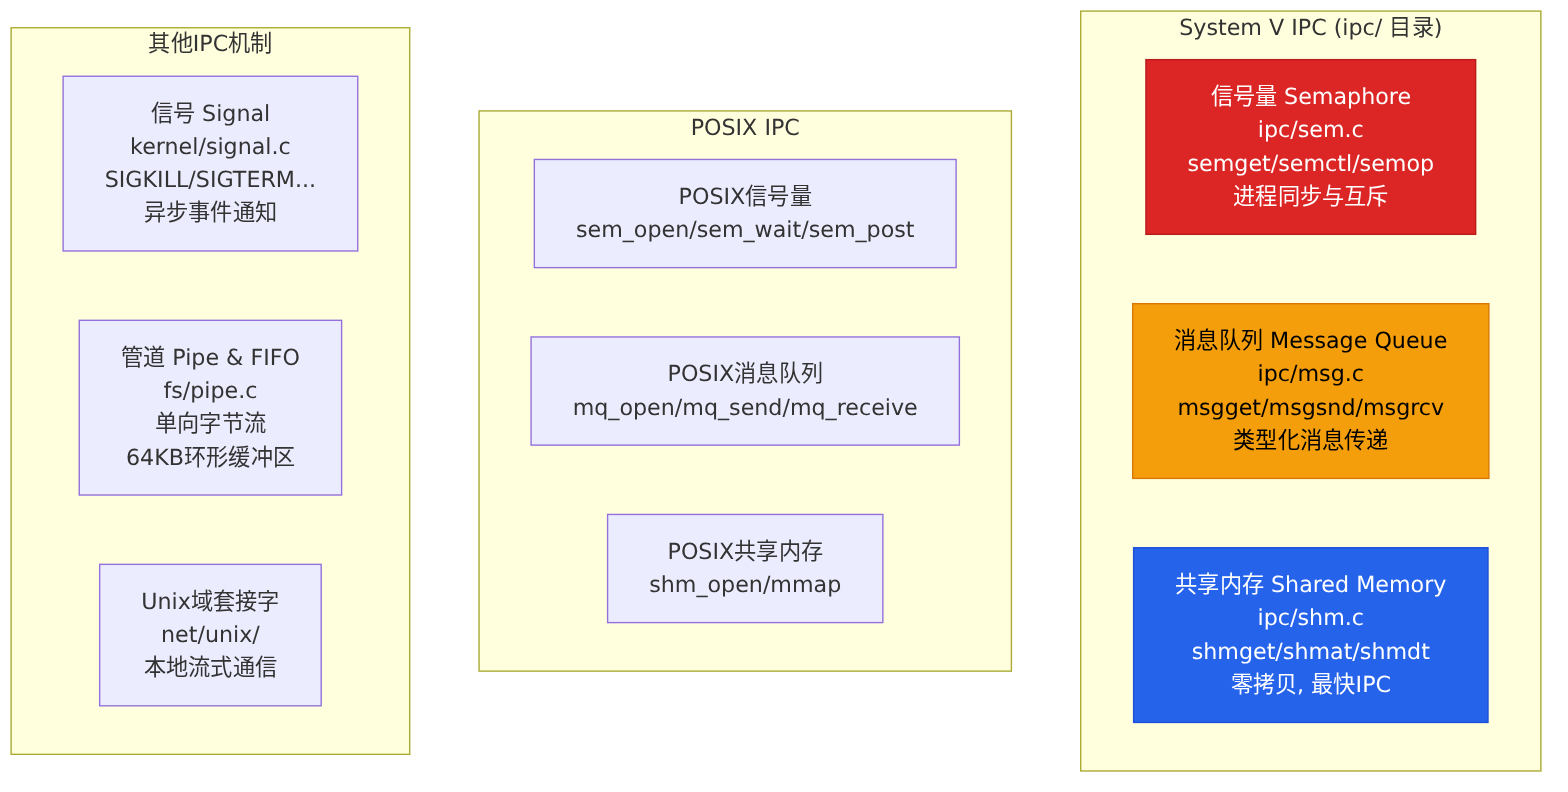
\includegraphics[width=0.85\textwidth]{fig_ch3_ipc_overview.png}
\caption{Linux 内核 IPC 机制总览}
\label{fig_ch3_ipc_overview}
\end{figure}

\subsection{信号量（Semaphore）}

\subsubsection{数据结构}

\begin{lstlisting}[language=C, caption={sem\_array 信号量集结构（ipc/sem.c）}, label={lst:sem_array}]
// ipc/sem.c
struct sem_array {
    struct kern_ipc_perm  sem_perm;     // IPC 权限结构
    time64_t              sem_ctime;    // 最后修改时间
    struct sem            sems[];        // 柔性数组：信号量数组
    struct list_head      pending_alter; // 等待 V 操作的队列链表
    struct list_head      pending_const; // 等待 0 操作的队列链表
    int                   complex_count;
};
struct sem {
    int    semval;     // 当前信号量值
    int    sempid;     // 最后操作该信号量的进程 PID
};
\end{lstlisting}

\subsubsection{semop() — P/V 操作调用链}

\texttt{semop()} 系统调用（\texttt{ipc/sem.c}）是信号量操作的核心入口。用户态通过 \texttt{semop(semid, sops, nsops)} 传递一个操作数组，内核需要保证这个操作数组的\textbf{原子性}——要么全部成功，要么全部不执行。这一语义是信号量实现进程间互斥同步的基础，也是 Dijkstra 经典 P/V 操作理论在内核中的直接映射。

系统调用入口 \texttt{sys\_semop() → do\_semop()} 首先通过 \texttt{sem\_obtain\_object\_check()} 根据 semid 查找 \texttt{struct sem\_array}，然后分配 \texttt{struct sem\_queue} 描述本次操作请求并将其挂入 \texttt{sem\_array} 的等待队列。核心决策函数 \texttt{perform\_atomic\_semop()} 遍历 semop 数组，对每个操作：若 \texttt{sop > 0}（V 操作）无条件将 \texttt{semval += sop}；若 \texttt{sop < 0}（P 操作）检查 \texttt{semval >= |sop|}，满足则 \texttt{semval -= sop}，否则标记失败。若有任一 P 操作失败，\textbf{回滚所有已执行的 V 操作}，恢复信号量原值。

若原子操作全部成功，立即返回用户态。若失败，调用进程被设置为 \texttt{TASK\_INTERRUPTIBLE} 状态，通过 \texttt{schedule\_timeout()} 让出 CPU 进入睡眠，等待后续 V 操作唤醒。当其他进程执行 \texttt{semop()} 中的 V 操作后，\texttt{update\_sem\_otime()} 遍历 \texttt{pending\_alter} 队列，对每个等待进程重新尝试 \texttt{perform\_atomic\_semop()}，成功则调用 \texttt{\_\_wake\_up\_common()} 将其唤醒。这一"完成后重试所有等待者"的机制保证了信号量的公平性——不会因为队列顺序导致某些进程饿死。

\subsubsection{从 Dijkstra PV 到 Linux semop：三层映射}

课本上的 PV 原语是抽象符号，实验中的 \texttt{sem\_p/sem\_v} 是用户态包装函数，内核中的 \texttt{perform\_atomic\_semop} 是真正执行者。以下从理论到实现做三层对照，理清每一层的语义变化：

\begin{table}[htbp]
\centering
\footnotesize
\caption{Dijkstra PV 原语 → XSI 信号量集 → 内核实现 三层映射}
\label{tab:pv_to_xsi}
\begin{tabular}{p{2.5cm}p{4cm}p{5.5cm}}
\toprule
\textbf{层次} & \textbf{P 操作（减量）} & \textbf{V 操作（增量）} \\
\midrule
\textbf{理论层}（Dijkstra, 1965）& \texttt{P(S): while(S<=0) wait; S--}——若资源不足则自旋等待，递减必须是原子操作 & \texttt{V(S): S++}——释放资源，若有等待者则唤醒 \\
\midrule
\textbf{用户态}（exp4 的 \texttt{sem\_p/sem\_v}）& \texttt{sb.sem\_op=-1; semop(semid, \&sb, 1)}——构造 \texttt{sembuf} 结构体，\texttt{sem\_op} 为负表示 P & \texttt{sb.sem\_op=+1; semop(semid, \&sb, 1)}——\texttt{sem\_op} 为正表示 V \\
\midrule
\textbf{内核态}（\texttt{ipc/sem.c}）& \texttt{perform\_atomic\_semop()} 第一遍遍历检查 \texttt{semval >= |sop|}，满足→第二遍执行 \texttt{semval -= |sop|}。不满足→\textbf{回滚已执行的所有操作}→\texttt{schedule\_timeout()} 睡眠 & \texttt{perform\_atomic\_semop()} 无条件 \texttt{semval += sop}→遍历 \texttt{pending\_alter} 队列→对每个等待者重试其操作集→成功则 \texttt{wake\_up\_process()} 唤醒 \\
\bottomrule
\end{tabular}
\end{table}

\textbf{关键细节——内核如何保证操作数组的整体原子性}。\texttt{semop()} 允许用户态一次提交多个操作（\texttt{nsops} 参数），这些操作必须\textbf{全部成功或全部不执行}。内核的 \texttt{perform\_atomic\_semop()} 采用类似银行家算法的"试分配"策略：

\begin{enumerate}[leftmargin=*]
    \item \textbf{第一遍——纯检查}：遍历 semop 数组。对每个 V 操作（\texttt{sop > 0}），无条件视为可行。对每个 P 操作（\texttt{sop < 0}），检查 \texttt{semval >= |sop|}。记录每个操作需要修改的量，但不实际修改 \texttt{semval}。
    \item \textbf{第二遍——执行+回滚}：若第一遍全部通过，遍历数组执行修改：V→\texttt{semval += sop}，P→\texttt{semval -= |sop|}。若任一 P 操作不满足条件，\textbf{回滚所有已执行的修改}（那些 V 操作的 \texttt{semval} 增量要减回去），然后整个操作集标记为"阻塞"，进程进入 \texttt{TASK\_INTERRUPTIBLE} 睡眠。
    \item \textbf{唤醒后重试}：当其他进程执行 V 操作后，内核遍历 \texttt{sma->pending\_alter} 链表，对每个等待的进程\textbf{从头重新执行完整的检查-执行流程}。这意味着一个进程在睡眠期间，它的"所需资源数"没有锁住任何资源——其他进程可以继续消费信号量，被唤醒的进程重新参与竞争。
\end{enumerate}

这套机制就是银行家算法在信号量领域的直接投影：银行家的安全序列检查 = \texttt{perform\_atomic\_semop} 的试分配+回滚；进程的 Need = \texttt{sembuf} 数组中的资源需求量；银行家的 Available = 信号量当前值 \texttt{semval}。区别在于信号量不需要预先声明最大需求——\texttt{semop} 数组本身就是"这次要多少"，不满足就睡等下次。

实验 4 的 \texttt{sem\_p/sem\_v} 每次只操作一个信号量（\texttt{nsops=1}），所以原子性保证仅体现在单变量上。实验 8 的死锁检测则直接修改了内核中同一个 \texttt{ipc/sem.c}，在 \texttt{semctl()} 中添加了遍历 \texttt{pending\_alter} 队列的逻辑——与 \texttt{perform\_atomic\_semop} 唤醒等待者时遍历的队列是同一个数据结构。

\subsection{共享内存（Shared Memory）}

共享内存是最高效的 IPC 机制，因为数据传输完全绕过了内核缓冲区（零拷贝）。其实现充分利用了 Linux 虚拟内存管理的惰性分配和缺页处理能力。

创建阶段：\texttt{shmget() → newseg()} 在内核中分配 \texttt{struct shmid\_kernel} 描述符，调用 \texttt{shmem\_alloc\_folio()} 从伙伴系统获取物理页框。但此时这些页框尚未映射到任何进程的地址空间——它们仅存在于内核的 page cache 中，等待后续缺页异常完成实际映射。

附加阶段：\texttt{shmat() → do\_shmat()} 调用 \texttt{do\_mmap()} 在进程地址空间中创建 VMA。此处关键设计在于 VMA 的 \texttt{vm\_ops} 被设置为 \texttt{shmem\_vm\_ops}，其中 \texttt{.fault = shmem\_fault}。这意味着进程首次访问共享内存地址时触发缺页异常，\texttt{handle\_mm\_fault() → do\_fault() → shmem\_fault()} 将之前分配的物理页框映射到进程页表中。这一惰性映射机制确保了即使分配了大量共享内存，未实际使用的页面不会消耗 TLB 条目。

分离阶段：\texttt{shmdt()} 仅从进程地址空间中解除 VMA 映射，不释放底层物理内存。物理页框持续存在直到显式调用 \texttt{shmctl(IPC\_RMID)} 删除共享内存段。这种"映射可断、数据不丢"的设计允许多个进程在各自的时间窗口内独立附加和分离同一共享内存段，非常适合长期运行的数据交换场景。

\subsection{信号（Signal）}

\textbf{发送路径}：\texttt{send\_signal() → \_\_send\_signal\_locked()}（\texttt{kernel/signal.c}），将 \texttt{struct sigqueue} 加入目标进程 \texttt{pending} 队列，调用 \texttt{complete\_signal()} → \texttt{signal\_wake\_up()} 设置 \texttt{TIF\_SIGPENDING} 并唤醒进程。

\textbf{处理路径}：进程从内核态返回用户态时检查 \texttt{TIF\_SIGPENDING}，调用 \texttt{arch\_do\_signal\_or\_restart()}（\texttt{arch/x86/kernel/signal.c}）→ \texttt{handle\_signal()}，在用户栈上构建信号帧（\texttt{setup\_rt\_frame()}），修改用户态 RIP 指向 handler 入口。handler 返回后通过 \texttt{sigreturn()} 恢复原执行上下文。

\textbf{信号交付本质上是一次"同进程内的用户态 mini context switch"。}这个过程需要在内核态和用户态之间做一次精密的控制转移，其复杂性不亚于调度器中的上下文切换，只是范围局限在单个进程内部。完整时序如下：

\begin{enumerate}[leftmargin=*]
    \item \textbf{保存现场}：内核在进程的用户栈上构造 \texttt{struct rt\_sigframe}，其中包含被打断时的全部通用寄存器（RAX/RBX/RCX/.../R15）、RIP（被打断的指令地址）、RSP（被打断时的用户栈指针）、RFLAGS，以及信号编号和附加信息（\texttt{siginfo\_t}）。
    \item \textbf{注入返回地址}：在信号帧中嵌入一个伪造的返回地址——它指向 vDSO 中的 \texttt{\_\_kernel\_rt\_sigreturn} 入口。这不是普通的函数返回地址，而是一个"陷阱"——handler 正常 \texttt{ret} 时就会落入这个地址，触发 \texttt{sigreturn()} 系统调用。
    \item \textbf{劫持控制流}：修改 \texttt{pt\_regs} 中的 RIP 指向信号 handler 的第一条指令，修改 RSP 指向信号帧上方（handler 使用的新栈区域）。由于这些修改发生在内核态的 \texttt{pt\_regs} 结构上，当进程通过 \texttt{sysretq} 返回用户态时，硬件自动从 \texttt{pt\_regs} 恢复 RIP/RSP——进程"看起来"像是在 handler 入口处开始执行。
    \item \textbf{handler 执行}：handler 在用户态运行，使用内核为其铺设的新栈区域。它可以访问 \texttt{siginfo\_t} 和 \texttt{ucontext\_t}（通过 handler 参数传入，指向信号帧中的对应区域）。
    \item \textbf{自动折返}：handler 执行 \texttt{ret} 指令。由于返回地址是 \texttt{\_\_kernel\_rt\_sigreturn}，CPU 跳转到 vDSO 中的 \texttt{syscall} 指令 → 进入内核 \texttt{sigreturn()} 系统调用。内核从用户栈上保存的 \texttt{rt\_sigframe} 中恢复全部通用寄存器、RIP、RSP、RFLAGS → \texttt{sysretq} → 进程回到被打断的原始位置，仿佛什么都没发生过。
\end{enumerate}

这个过程和调度器上下文切换的对称性值得注意：调度器的 \texttt{\_\_switch\_to\_asm} 在\textbf{内核栈}上保存/恢复寄存器，切换的是\textbf{两个不同进程}的执行流；信号交付在\textbf{用户栈}上保存/恢复寄存器，切换的是\textbf{同一进程的两个用户态上下文}（主执行流和信号 handler）。两者都依赖"在某处保存全量寄存器状态→修改 RIP→未来从保存点恢复"的机制，只是载体不同。

\begin{figure}[htbp]
\centering
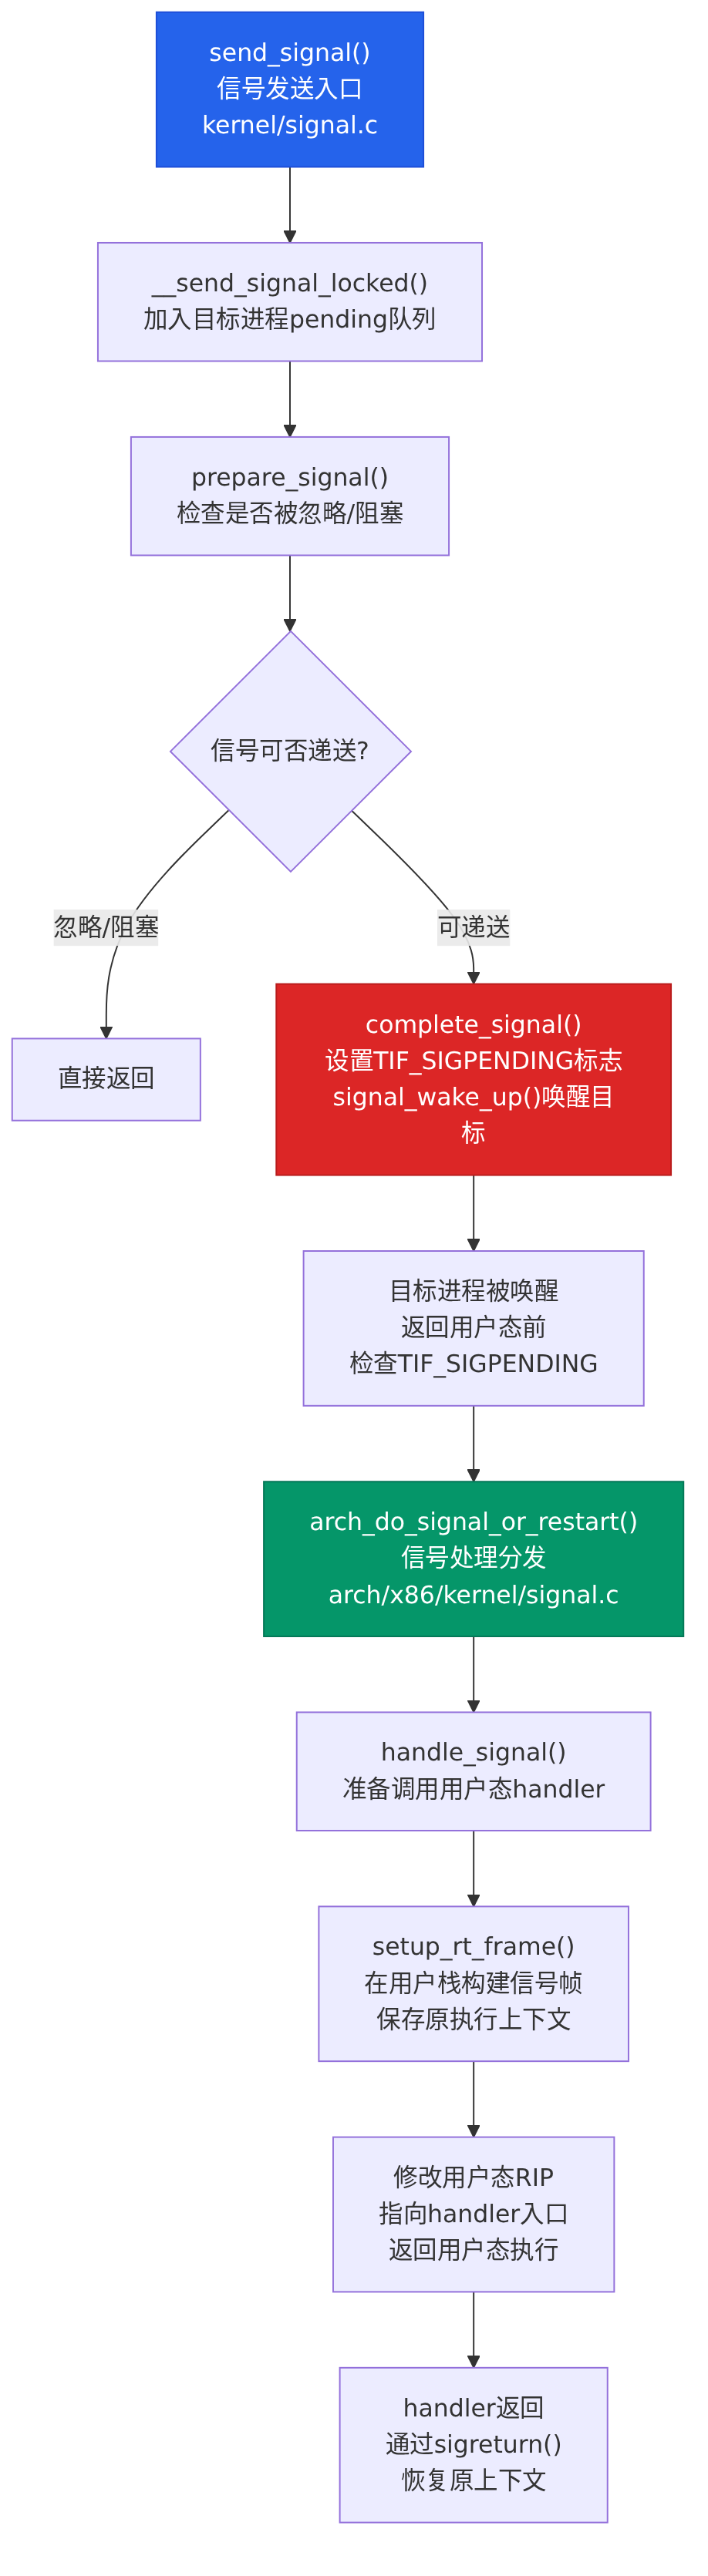
\includegraphics[height=0.88\textheight]{fig_ch3_signal_flow.png}
\caption{Linux 信号发送与处理流程}
\label{fig_ch3_signal_flow}
\end{figure}

\subsection{管道（Pipe）}

管道（\texttt{fs/pipe.c}）是 Unix 最经典的 IPC 机制，实现为内核中的环形缓冲区。默认容量为 16 个页（64KB），可通过 \texttt{fcntl(F\_SETPIPE\_SZ)} 调整。管道的数据结构 \texttt{struct pipe\_inode\_info} 包含一个 \texttt{struct pipe\_buffer} 数组（环形缓冲区的槽位）和读写指针。

\texttt{pipe\_write()} 的调用链为 \texttt{ksys\_write() → vfs\_write() → pipe\_write()}。写入操作首先检查管道是否已有读端关闭（若关闭则发送 SIGPIPE 信号），然后通过 \texttt{pipe\_get\_tx\_ring\_size()} 获取可用空间。若管道有足够空间容纳写入数据，\texttt{copy\_page\_from\_iter()} 将用户空间数据复制到内核中的 pipe buffer 页面；若管道满，根据 \texttt{O\_NONBLOCK} 标志决定是否阻塞——阻塞模式下写入进程进入 \texttt{TASK\_INTERRUPTIBLE} 睡眠，等待读端消费数据后通过 \texttt{poll\_wake()} 唤醒。

\texttt{pipe\_read()} 执行对称操作：检查管道是否有数据，若有则通过 \texttt{copy\_page\_to\_iter()} 将内核 pipe buffer 数据复制到用户空间缓冲区，更新读指针；若管道空则根据 \texttt{O\_NONBLOCK} 决定阻塞或立即返回 -EAGAIN。

管道的核心设计限制是\textbf{半双工}——数据只能单向流动。若需要双向通信，通常创建一对管道或使用 Unix Domain Socket。管道的最大优势在于其简单性和与 shell 管线的无缝集成（\texttt{pipe() + fork() + dup2() + exec()} 的经典模式），使得进程间数据流式处理无需任何显式的同步原语——管道的 FIFO 顺序和阻塞语义天然提供了生产者-消费者同步。

\subsection{实验验证}

\subsubsection{实验4：生产者-消费者多进程实现}

本实验使用 System V IPC 实现了 3 生产者 + 4 消费者的经典多进程同步模型。核心设计：共享环形缓冲区（容量 8）通过 XSI 信号量集的三个信号量保护——\texttt{MUTEX}（互斥锁，初值 1）、\texttt{EMPTY}（空槽计数，初值 8）、\texttt{FULL}（满槽计数，初值 0）。生产者流程为 \texttt{P(EMPTY) → P(MUTEX) → 写入 → V(MUTEX) → V(FULL)}，消费者流程为 \texttt{P(FULL) → P(MUTEX) → 读取 → V(MUTEX) → V(EMPTY)}。共享缓冲区通过 \texttt{shmget() + shmat()} 映射到各进程地址空间。

关键技术细节：\texttt{fork()} 之前调用 \texttt{setvbuf(stdout, NULL, \_IONBF, 0)} 禁用 stdio 缓冲，避免 fork 后子进程复制缓冲区导致输出重复；消费者退出前执行级联唤醒——检测到总消费量已达目标后额外执行一次 \texttt{V(FULL)}，防止最后一个消费者阻塞在 \texttt{P(FULL)} 上无人唤醒。

验证结果：3 生产者各生产 5 项（总计 15），4 消费者共消费 15 项，缓冲区残留为 0，所有 7 个子进程正常退出。多次运行结果一致，确认无死锁、无活锁、无数据竞争。该实验直接验证了 §3.2 所述的信号量 P/V 原子操作——\texttt{semop()} 系统调用进入 \texttt{ipc/sem.c} 中的 \texttt{perform\_atomic\_semop()}，通过原子操作集语义保证了要么全部成功要么全部回滚。

\subsubsection{实验8：信号量死锁检测与解除}

本实验对内核 \texttt{ipc/sem.c} 进行了功能性扩展，添加了两个自定义 \texttt{semctl} 命令。\texttt{detect\_sem\_deadlock()}（DEADCHECK = 0xDEAD）的检测逻辑为：遍历信号量集中的全部信号量，若每个 \texttt{semval} 均为 0 且阻塞等待进程数 ≥ 2 且 ≥ 信号量数，则判定为潜在死锁。\texttt{break\_sem\_deadlock()}（DEADBREAK = 0xBEAC）选择等待队列中 RSS 最小的进程（作为"代价最小"的受害者），通过 \texttt{kill\_pid(task\_pid(victim), SIGKILL, 1)} 强制终止以打破环路。

开发过程中修复了两个关键 bug：一是最初只扫描全局等待队列 \texttt{sma->pending\_alter}，遗漏了 per-信号量等待队列 \texttt{sma->sems[i].pending\_alter}；二是 glibc 的 \texttt{semctl()} 包装函数在用户态检查 \texttt{cmd} 参数并拒绝未知值——\texttt{semctl(semid, 0, 0xDEAD)} 根本未进入内核，需改用 \texttt{syscall(\_\_NR\_semctl, ...)} 直接调用。

验证测试构造了经典的 AB-BA 死锁（P1 持有 sem[0] 等待 sem[1]，P2 持有 sem[1] 等待 sem[0]），DEADCHECK 成功返回 1（检测到死锁），DEADBREAK 成功返回 0 并终止 RSS 较小的进程。内核日志输出 \texttt{"[sem\_deadlock] DEADLOCK DETECTED! semid=65538 waiters=2 nsems=2"}。该实验验证了死锁检测算法在真实内核 IPC 子系统中的实现可行性。

%========================================== 第4章 ==========================================
\section{物理内存管理和分配机制} \label{sec:ch4}

\subsection{NUMA 与内存节点}

在 NUMA 架构下，物理内存按节点（node）、区域（zone）两级组织\cite{gorman}。NUMA 的核心思想是"本地内存访问快、远端内存访问慢"——每个 CPU 直接连接一部分物理内存（本地节点），访问该节点的内存延迟最低；跨节点访问需要经过 CPU 间互联总线，延迟显著增加（在大型服务器上可达 1.5–3 倍）。

每个节点由 \texttt{pglist\_data} 结构描述（\texttt{include/linux/mmzone.h}）。该结构包含节点 ID、节点起始页框号 \texttt{node\_start\_pfn}、节点拥有的物理页数 \texttt{node\_present\_pages}、以及该节点上的所有 zone 数组 \texttt{node\_zones[MAX\_NR\_ZONES]}。关键的 \texttt{node\_zonelists} 定义了该节点进行内存分配时的 zone 遍历顺序——优先从本节点的 ZONE\_NORMAL 分配，若不足再尝试本节点的 ZONE\_DMA32，最后才回退到远端节点的内存。这一"本地优先、远端兜底"的策略在整个伙伴系统的 \texttt{get\_page\_from\_freelist()} 中通过遍历 \texttt{zonelist} 自动贯彻。

在 x86\_64 架构下，每个节点内部划分四个区域：\texttt{ZONE\_DMA}（0–16MB，传统 ISA 设备 DMA 需要物理地址在此范围）、\texttt{ZONE\_DMA32}（16MB–4GB，32 位 PCI 设备 DMA 限制）、\texttt{ZONE\_NORMAL}（4GB 以上至内核直接映射上限 \texttt{PAGE\_OFFSET + 64TB}，内核通过 \texttt{\_\_va()/\_\_pa()} 宏实现虚拟地址与物理地址的 O(1) 转换）、\texttt{ZONE\_MOVABLE}（用于内存热插拔和碎片整理的可迁移页面区域）。区域划分使得内核在分配时可以根据请求的 gfp 标志（如 \texttt{GFP\_DMA, GFP\_DMA32, GFP\_HIGHUSER\_MOVABLE}）精确选择满足硬件约束的物理内存。

\subsection{伙伴系统（Buddy System）}

伙伴系统是 Linux 物理页分配的基础算法（\texttt{mm/page\_alloc.c}），管理 \texttt{MAX\_ORDER - 1 = 10} 个阶（order 0–10，即 1 页至 1024 页连续块）\cite{gorman,mm_doc}。

\subsubsection{核心数据结构}

\begin{lstlisting}[language=C, caption={free\_area — 伙伴系统空闲链表（include/linux/mmzone.h）}, label={lst:free_area}]
struct free_area {
    struct list_head free_list[MIGRATE_TYPES];  // 按迁移类型分类
    unsigned long nr_free;                       // 该阶空闲块数量
};
struct zone {
    struct free_area free_area[MAX_ORDER];      // 各阶空闲链表
    unsigned long managed_pages;
    // ...
};
\end{lstlisting}

\subsubsection{分配路径详解}

页分配的主入口为 \texttt{alloc\_pages()}，最终进入 \texttt{\_\_alloc\_pages\_noprof()}（\texttt{mm/page\_alloc.c}）。该函数首先通过 \texttt{prepare\_alloc\_pages()} 设置分配上下文（gfp\_t 标志位决定分配行为：\texttt{GFP\_KERNEL} 允许睡眠和回收、\texttt{GFP\_ATOMIC} 禁止睡眠、\texttt{\_\_GFP\_HIGH} 允许使用紧急保留内存等）。

随后进入\textbf{快速路径}——\texttt{get\_page\_from\_freelist()}：该函数遍历 \texttt{zonelist}（区域优先级列表），在每个 zone 中查找 \texttt{free\_area[order]}。若请求的 order 有空闲块，调用 \texttt{\_\_rmqueue()} 从链表中取出。\texttt{\_\_rmqueue()} 的关键优化是先在新添加的 MIGRATE 类型（如 \texttt{MIGRATE\_UNMOVABLE}, \texttt{MIGRATE\_RECLAIMABLE}, \texttt{MIGRATE\_MOVABLE}）对应链表中查找，这一机制通过将不同生命周期的页面分类存储来减少内存碎片。若请求阶数无空闲块，调用 \texttt{\_\_rmqueue\_fallback()} 向高阶借块——将 $2^{k+1}$ 的伙伴块按地址一分为二，低地址半部用于分配，高地址半部作为 $2^k$ 阶块归还低阶链表（\texttt{expand()} 函数执行此分裂）。

若快速路径失败，进入\textbf{慢速路径}——\texttt{\_\_alloc\_pages\_slowpath()}：首先尝试异步内存压缩（\texttt{should\_compact\_retry()} + \texttt{try\_to\_compact\_pages()}），将分散的空闲页聚集为高阶连续块；若仍不足，唤醒 \texttt{kswapd} 执行页面回收，将 Inactive 链表中的页面换出以释放物理页。经过多轮重试（最多 \texttt{MAX\_RECLAIM\_RETRIES} 次），若所有努力均无法满足分配请求且 \texttt{gfp\_t} 中设置了 \texttt{\_\_GFP\_RETRY\_MAYFAIL} 以外的标志，则 OOM killer 选择并终止内存消耗最大的进程。

\subsubsection{释放路径详解}

\texttt{\_\_free\_pages()} 是页释放的主入口。释放路径的精妙之处在于\textbf{伙伴合并}：函数 \texttt{\_\_free\_one\_page()} 将待释放页框加入对应 order 的空闲链表，然后调用 \texttt{\_\_find\_buddy\_pfn()} 计算伙伴页框号。在伙伴系统中，两个页框互为伙伴当且仅当：它们的页框号仅在第 order 位不同（即 \texttt{pfn \textasciicircum (1 << order)}）。通过简单的位运算即可快速定位伙伴，无需遍历链表。

若伙伴同阶且空闲——即满足 \texttt{page\_is\_buddy()} 检查（伙伴不在使用中、同阶、同 zone），则将两个 order-k 伙伴从空闲链表中移除，合并为一个 order-(k+1) 块，然后递归尝试与新的伙伴合并。这一过程持续到无法再合并为止——此时所有可合并的伙伴均已聚合为最大连续块，最大化了大块连续物理内存的可用性。

\textbf{伙伴系统的根本缺陷与 MIGRATE\_TYPES 的补救。}理论上伙伴系统的外部碎片率不超过 33\%，但实践中远不止此。问题出在页面生命周期的异质性：内核通过 \texttt{GFP\_KERNEL} 分配的页面（如 \texttt{kmalloc} 的对象、页表页）在整个系统运行期间散布在各处且无法迁移。当一个不可移动页恰好落在两个可合并的伙伴之间时，合并链被切断——该页两侧的大块永远无法聚合，即使系统有大量空闲内存也凑不出高阶连续块。Linux 通过 \textbf{MIGRATE\_TYPES} 机制缓解此问题：将空闲页面按迁移属性分为 \texttt{MIGRATE\_UNMOVABLE}（内核核心分配，不可移动）、\texttt{MIGRATE\_RECLAIMABLE}（可回收，如 inode/dentry cache）、\texttt{MIGRATE\_MOVABLE}（用户态页面，可通过缺页异常迁移）、\texttt{MIGRATE\_CMA}（连续内存分配器专用）等类型。\texttt{\_\_rmqueue()} 分配时优先在匹配的迁移类型链表中查找，同类页面聚集在一起，碎片只发生在同类型内。但还有一个更深的问题：\texttt{MIGRATE\_UNMOVABLE} 区域会随时间逐渐扩张（内核分配无处不在），侵蚀可移动区域。\texttt{memory compaction}（\texttt{mm/compaction.c}）正是为此存在——它主动迁移 \texttt{MIGRATE\_MOVABLE} 页面到其他位置，为不可移动分配腾出连续空间。实验 10 的 \texttt{page\_stats.ko} 逐页遍历时通过 \texttt{PageBuddy/PageSlab/PageLRU} 等宏分类统计，正是对这几种迁移类型的间接观测。

\figref{fig_ch4_page_alloc} 展示了伙伴系统分配与释放的完整流程。

\begin{figure}[htbp]
\centering
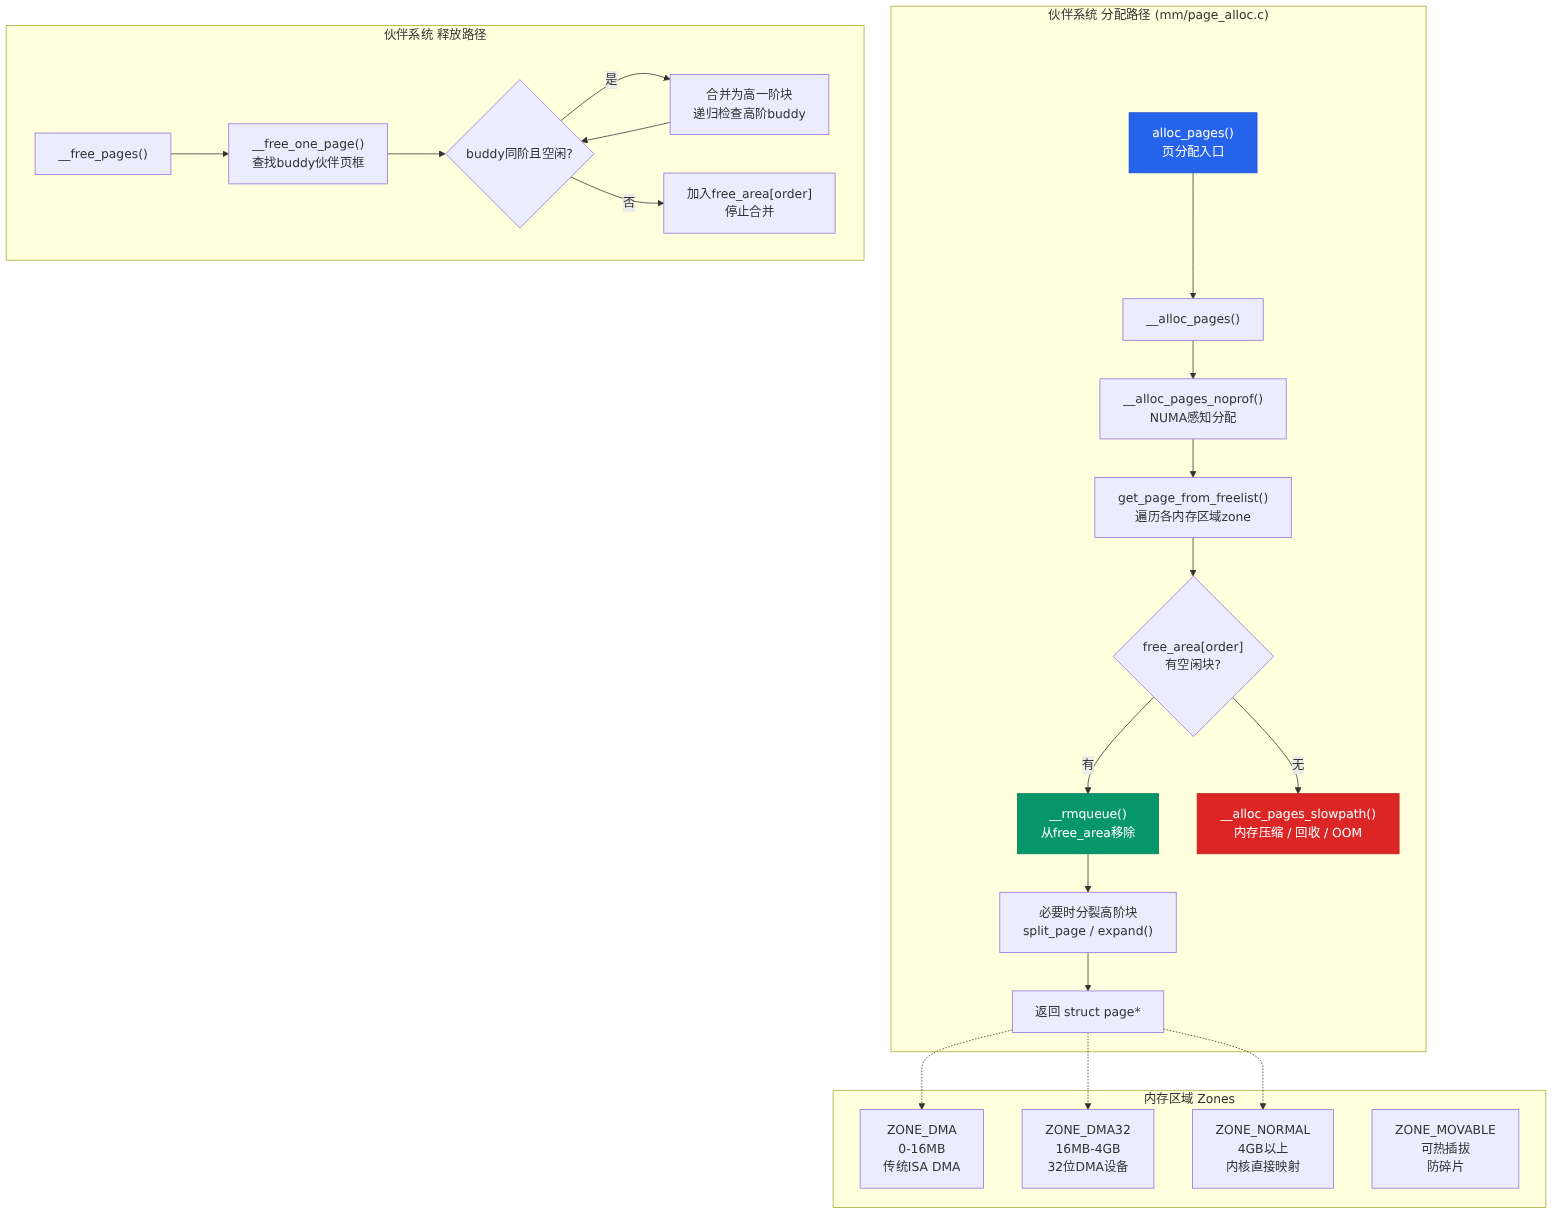
\includegraphics[width=0.95\textwidth,height=0.88\textheight,keepaspectratio]{fig_ch4_page_alloc.png}
\caption{伙伴系统页分配与释放流程}
\label{fig_ch4_page_alloc}
\end{figure}

\subsection{Slub 分配器}

伙伴系统以页为分配粒度，对于内核中频繁使用的小对象（如 \texttt{task\_struct}, \texttt{inode}, \texttt{dentry}），Linux 使用 slub 分配器（\texttt{mm/slub.c}）\cite{mckenney}。每个 slab 缓存（\texttt{struct kmem\_cache}）管理特定大小的对象，通过 \texttt{kmem\_cache\_alloc()} / \texttt{kmem\_cache\_free()} 进行快速分配和释放。slub 分配器从伙伴系统获取大块页面，内部细分为等大小的对象槽位，利用 per-CPU 缓存实现无锁快速路径。

\subsection{实验验证}

\subsubsection{实验10：内存管理分析与验证（物理内存部分）}

本实验通过三个用户态程序和一个内核模块对第 4–5 章的内存管理理论进行了系统验证。

\texttt{mem\_observe.c} 通过 \texttt{strace -e trace=brk,mmap,munmap} 跟踪 \texttt{malloc()} 的底层行为，精确测定了 glibc 的分配策略阈值：≤64KB 时使用 \texttt{brk()} 扩展堆区（连续地址，无法单独释放中间块）；≥1MB 时使用 \texttt{mmap()} 匿名映射（独立 VMA，可独立 \texttt{munmap}）；过渡区间 64KB–1MB 根据 glibc 内部策略动态选择。该观察直接印证了 §4.2 和 §5.2 所述的两种内存分配路径。

\texttt{mem\_alloc.c} 通过 \texttt{mmap} 20000 个 4KB 页面（共 80MB）对比两种场景验证惰性分配：只 \texttt{mmap} 不访问时 VIRT 增长 80MB 但 RES 几乎不变——页表项为空，未触发缺页；调用 \texttt{memset} 逐页写入后 RES 与 VIRT 同步增长至 ~80MB——每次首次写入触发一次缺页异常 → \texttt{do\_anonymous\_page()} 分配物理页框。该实验直观展示了虚拟内存惰性分配的"承诺 vs 兑现"机制。

\texttt{page\_stats.ko} 内核模块遍历所有 NUMA 节点和内存区域，通过 \texttt{pfn\_to\_page()} 逐页统计使用 \texttt{PageBuddy/PageSlab/PageLRU/folio\_test\_active/PageTable/PageReserved} 等宏分类。Linux 6.18 中需使用 folio API（\texttt{folio\_test\_active(page\_folio(page))} 替代已废弃的 \texttt{PageActive()}），且 \texttt{first\_online\_pgdat()/next\_online\_pgdat()} 未导出，需改用 \texttt{for\_each\_online\_node(nid) + NODE\_DATA(nid)} 遍历。模块输出与 \texttt{/proc/meminfo} 数据吻合，验证了伙伴系统各阶空闲块的分布与内核页面统计的一致性。

%========================================== 第5章 ==========================================
\section{虚拟存储管理和换页机制} \label{sec:ch5}

\subsection{虚拟地址空间管理}

进程的虚拟地址空间由 \texttt{struct mm\_struct}（\texttt{include/linux/mm\_types.h}）描述\cite{bovet,gorman}。其中包含 VMA 链表（\texttt{mmap}）和红黑树（\texttt{mm\_rb}）用于快速查找地址对应的 VMA，以及页全局目录指针（\texttt{pgd}）指向进程页表根。

\subsection{vm\_area\_struct（VMA）}

每个 VMA 描述进程地址空间中一段连续的虚拟地址区间：

\begin{lstlisting}[language=C, caption={vm\_area\_struct 核心字段（include/linux/mm\_types.h）}, label={lst:vma}]
struct vm_area_struct {
    unsigned long vm_start;        // 区间起始虚拟地址
    unsigned long vm_end;          // 区间结束虚拟地址
    pgprot_t vm_page_prot;        // 页保护属性
    unsigned long vm_flags;        // VM_READ|VM_WRITE|VM_EXEC|VM_SHARED...
    const struct vm_operations_struct *vm_ops;  // VMA 操作回调
    unsigned long vm_pgoff;        // 文件映射偏移（页单位）
    struct file *vm_file;          // 文件映射的 struct file
    struct mm_struct *vm_mm;       // 所属 mm_struct
    struct rb_node vm_rb;          // 红黑树节点
};
\end{lstlisting}

\subsection{mmap 系统调用与惰性分配}

\texttt{mmap() → do\_mmap()}（\texttt{mm/mmap.c}）是创建虚拟内存映射的核心入口\cite{lwn_mm}。\texttt{mmap\_region()} 分配 \texttt{vm\_area\_struct} 并设置地址范围、权限、文件映射信息，通过 \texttt{vma\_link()} 插入 \texttt{mm->mmap} 链表和 \texttt{mm->mm\_rb} 红黑树。

\textbf{关键设计——惰性分配}：\texttt{mmap()} 仅创建 VMA 记录映射关系，不立即分配物理页。进程首次访问该地址时触发缺页异常，由 \texttt{handle\_mm\_fault()} 完成页表项的实际填充。这极大节省了物理内存，如\figref{fig_ch5_vma_mmap}所示。

\begin{figure}[htbp]
\centering
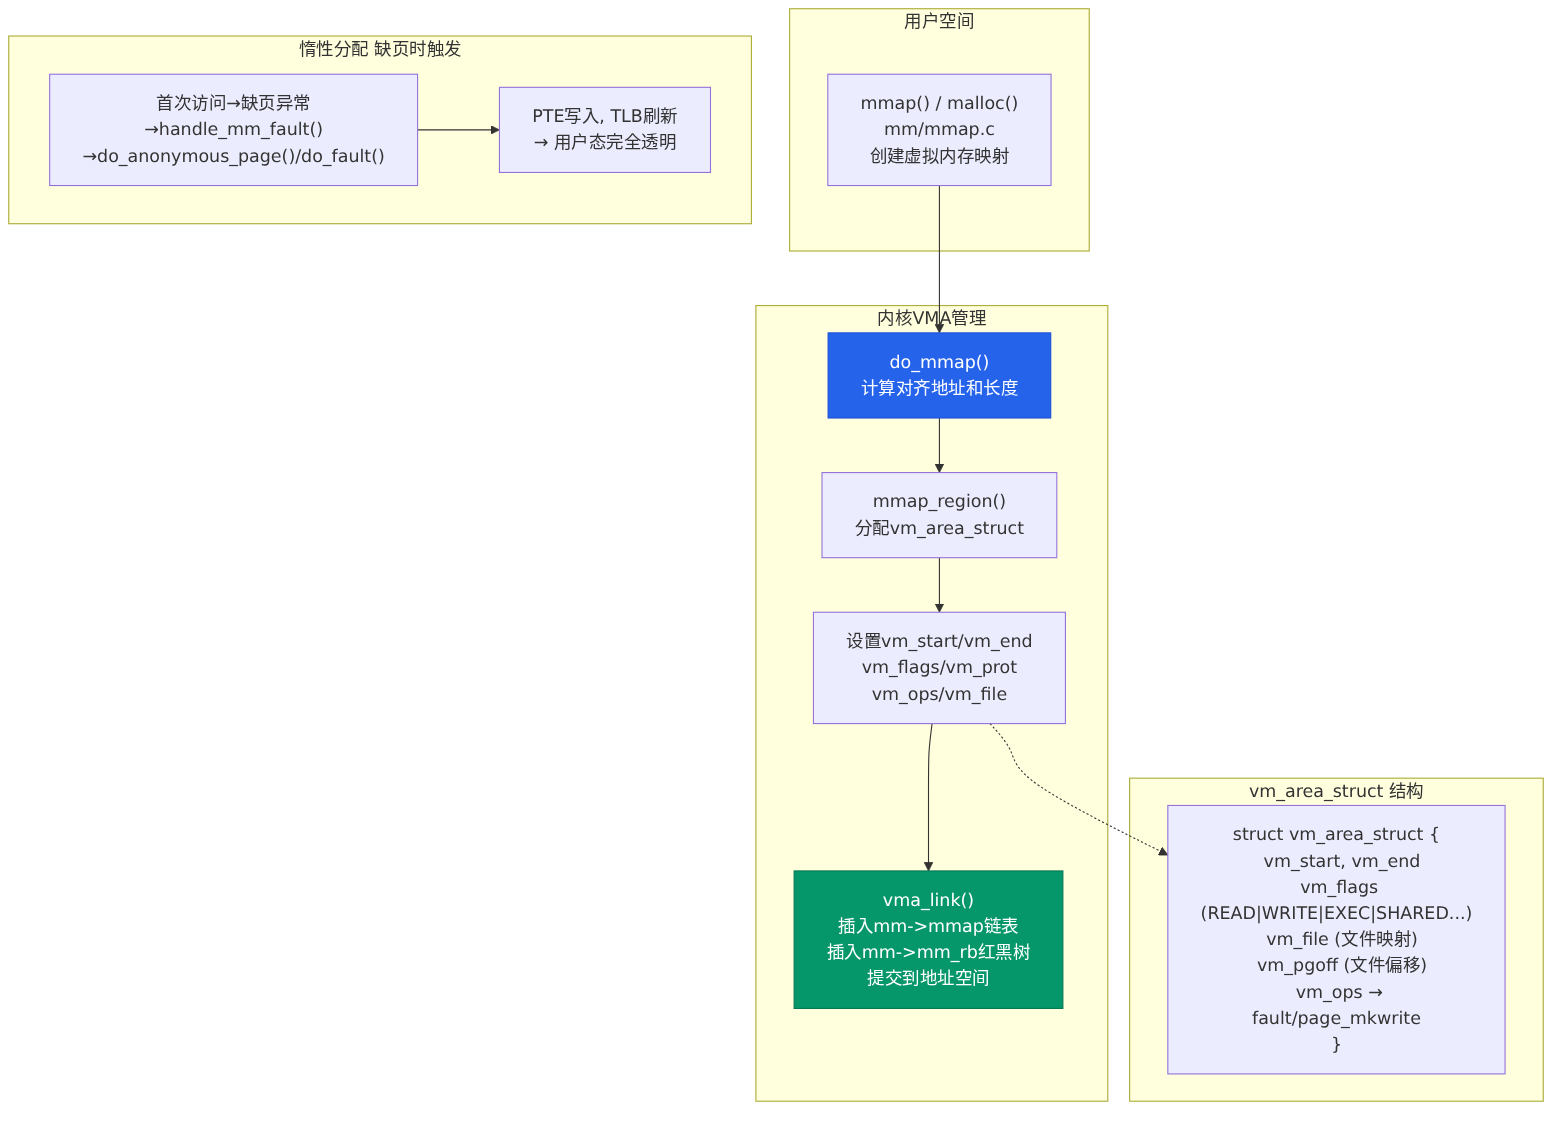
\includegraphics[width=0.85\textwidth]{fig_ch5_vma_mmap.png}
\caption{mmap 系统调用与 VMA 惰性分配机制}
\label{fig_ch5_vma_mmap}
\end{figure}

\subsection{缺页异常处理}

x86\_64 下缺页异常由 IDT 表项 \texttt{exc\_page\_fault} 调用 \texttt{handle\_page\_fault()}（\texttt{arch/x86/mm/fault.c}），从 CR2 获取 fault 地址、解析 \texttt{error\_code}，分发至 \texttt{handle\_mm\_fault()}（\texttt{mm/memory.c}）\cite{lwn_page_fault}。

\texttt{handle\_mm\_fault()} 完成五级页表遍历（pgd→p4d→pud→pmd→pte），根据 PTE 状态分发。值得深入分析的是各级页目录的\textbf{按需分配}机制：内核在遍历过程中可能发现某级页目录不存在（如 pgd 条目为空），此时调用 \texttt{p4d\_alloc()}、\texttt{pud\_alloc()}、\texttt{pmd\_alloc()} 逐级分配中间页表。这一懒分配策略与 VMA 的惰性分配一脉相承——只有真正需要写入页表条目时才分配中间页目录的内存。分配完所有中间目录后，到达最终 PTE 层，根据具体状态走四种路径之一：

\begin{itemize}[leftmargin=*]
    \item \textbf{PTE 为空（首次访问）}：\texttt{do\_anonymous\_page()} 处理匿名映射的首次访问。对于读访问，分配一个全零的"零页"（\texttt{ZERO\_PAGE}）并映射为只读——所有仅读取而未写入的匿名页共享同一个物理零页，节省内存。对于写访问，通过伙伴系统分配新物理页框并清零（防止信息泄露），设置 PTE 为可写，完成从虚拟地址到物理页框的绑定。若此匿名页由 \texttt{fork()} 的 COW 产生，则标记为写保护。

    \item \textbf{PTE 为 swap 条目}：\texttt{do\_swap\_page()} 处理被换出页面的重新访问。swap 条目中编码了 swap 设备号和槽位偏移，内核通过 \texttt{lookup\_swap\_cache()} 或 \texttt{read\_swap\_cache\_async()} 从 swap 设备读回页面数据。若该页面同时存在于 swap cache（其他进程恰好也在换入同一页），则直接共享 page cache 中的页面，避免重复 I/O。

    \item \textbf{PTE 为文件页}：\texttt{do\_fault()} 处理文件映射（mmap 的文件页或 ELF 可执行文件的代码段）。数据流为：\texttt{do\_fault() → do\_read\_fault() → \_\_do\_fault() → vmf->vma->vm\_ops->fault()}。以 ext2 文件映射为例，最终调用 \texttt{filemap\_fault()}，在 page cache 中查找文件偏移对应的 page，若未命中则调用 \texttt{ext2\_read\_folio()} 从磁盘读取数据填充新 page。

    \item \textbf{PTE 存在但写保护（COW）}：\texttt{do\_wp\_page()} 处理写时复制。这是 fork 后父子进程共享页面的关键技术，详见下一小节的深入分析。
\end{itemize}

\figref{fig_ch5_page_fault} 展示了缺页异常处理的完整决策树。

\begin{figure}[htbp]
\centering
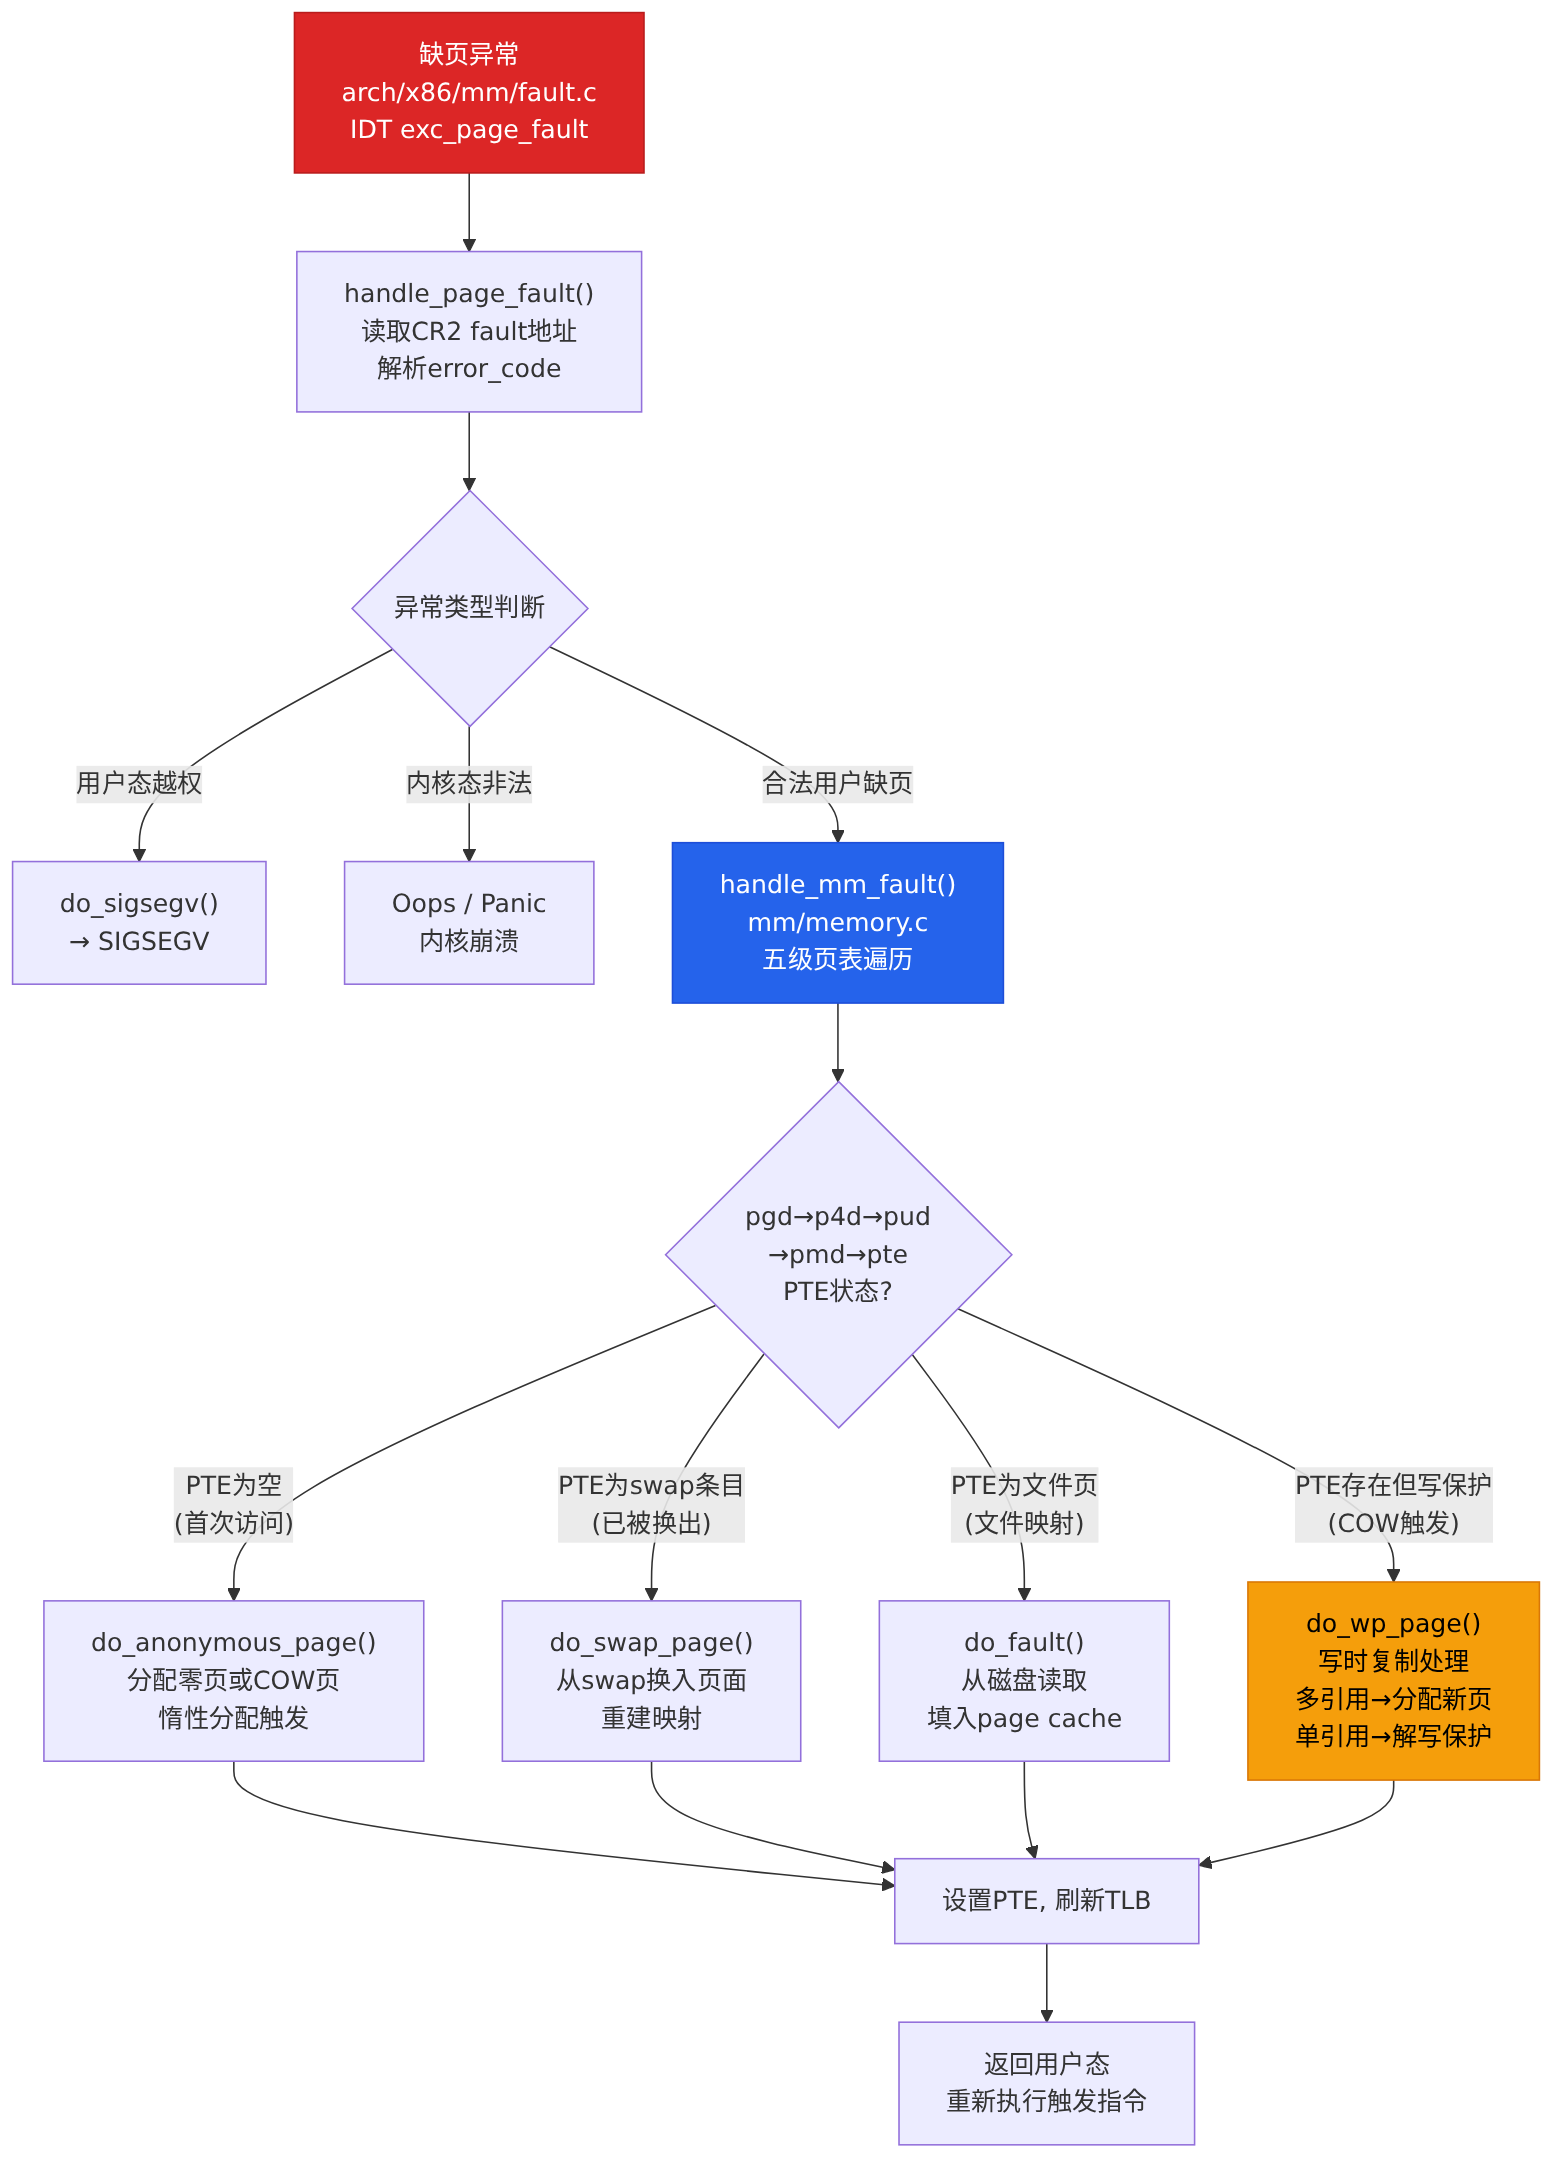
\includegraphics[width=0.95\textwidth,height=0.88\textheight,keepaspectratio]{fig_ch5_page_fault.png}
\caption{缺页异常处理完整流程}
\label{fig_ch5_page_fault}
\end{figure}

\subsection{Copy-on-Write（COW）深入分析}

COW 是 Linux 虚拟内存管理的核心优化\cite{bovet}。在 \texttt{fork()} 期间，\texttt{copy\_mm() → dup\_mmap()} 复制父进程的所有 VMA，将父子进程的页表项均标记为只读并设置 \texttt{PTE\_SOFT\_DIRTY}。任一进程尝试写入共享页时触发写保护缺页，\texttt{do\_wp\_page()}（\texttt{mm/memory.c}）执行：

\begin{lstlisting}[language=C, caption={do\_wp\_page 核心逻辑（mm/memory.c）}, label={lst:do_wp_page}]
static vm_fault_t do_wp_page(struct vm_fault *vmf) {
    // 1. 获取缺页所在的 VMA 和页表项
    vma = vmf->vma;
    // 2. 获取物理页 folio
    folio = page_folio(vmf->page);
    // 3. ★ 关键判断：folio 的引用计数
    if (folio_likely_mapped_shared(folio)) {
        // 多个进程共享 → 必须分配新页、复制内容
        new_folio = folio_copy(folio, vma, vmf->address);
        page_add_new_anon_rmap(new_folio, vma, vmf->address);
    } else {
        // 仅一个使用者 → 直接在原页上解除写保护
        wp_page_reuse(vmf);
        folio_mark_accessed(folio);
    }
    // 4. 更新页表项为可写，刷新 TLB
}
\end{lstlisting}

\textbf{关键优化}：若 \texttt{folio\_ref\_count == 1}（已无其他使用者，如父进程退出后子进程独占），直接在原页上解除写保护而无需复制，避免了不必要的内存分配和拷贝开销。

\textbf{COW 的工程经济学：为什么 fork+exec 组合几乎免费。}COW 最重要的设计动机不是节省 fork 后的写入——而是让 fork 后立即 exec 的场景不浪费任何物理内存。考虑 shell 执行 \texttt{ls} 的典型流程：

\begin{itemize}[leftmargin=*]
    \item \texttt{bash}（200MB 常驻内存）调用 \texttt{fork()}。不用 COW 的话，需要立即分配 200MB 物理内存并逐页复制内容。然后 \texttt{exec("ls")} 调用 \texttt{flush\_old\_exec() → exec\_mmap()} 释放整个地址空间——200MB 的分配和复制全部作废。
    \item 用 COW：\texttt{fork()} 只复制页表。bash 的 200MB 地址空间按 4KB 分页，共约 51,200 个 PTE，每个 PTE 8 字节，页表复制开销约 400KB。父子进程的页表项均标记为只读（\texttt{PTE\_RDONLY | PTE\_SOFT\_DIRTY}），但物理页框不做任何复制——父子共享全部 200MB 物理页。
    \item \texttt{exec("ls")} 调用 \texttt{exec\_mmap() → mmput(old\_mm)}，旧 mm\_struct 的引用计数递减。页表被释放（400KB 回收），但物理页框因为 bash 父进程仍持有引用而不释放。子进程从未写入过任何共享页——\textbf{零 COW 缺页发生}。
    \item 总开销：400KB 的页表复制 + 释放。与父进程内存大小无关。
\end{itemize}

这个设计使得 Unix 的"fork+exec 创建新进程"模式在工程上可行——否则每次敲命令都要复制整个 shell 的内存，200MB 的 bash 会让系统寸步难行。实验 10 的 \texttt{mem\_cow.c} 通过 \texttt{/proc/<pid>/smaps} 观察 PSS（Proportional Set Size）值验证了此机制：fork 后父子 PSS 各为原值的一半（共享页按引用计数均分），子进程写入后才各自增长为独立物理页的完整值。

当系统内存压力增大时，\texttt{kswapd} 守护线程被唤醒执行页面回收（\texttt{mm/vmscan.c}）。回收策略：遍历 LRU 链表（Active/Inactive × Anonymous/File 四个链表），优先回收 Inactive 端页面。匿名页通过 \texttt{add\_to\_swap()} 分配 swap 槽位写入 swap 设备，PTE 替换为 swap 条目。文件页若干净可直接丢弃（可从磁盘重读），若脏页先调用 \texttt{writepage()} 写回。

\subsection{实验验证}

\subsubsection{实验10：内存管理分析与验证（虚拟内存部分）}

\texttt{mem\_cow.c} 是验证写时复制机制的核心测试程序。父进程通过 \texttt{mmap(MAP\_PRIVATE|MAP\_ANONYMOUS|MAP\_POPULATE, size)} 分配 N GB 内存并 \texttt{memset} 写入初始值（强制触发所有页面的缺页分配），然后 \texttt{fork()}。fork 后通过 \texttt{top} 观察：父子进程 VIRT 各显示 N GB，但系统总 RES 仅增长至 ~N GB（而非 2N GB）——父子共享相同的物理页框，页表项均标记为只读。子进程随后 \texttt{memset} 写入前一半页面，触发 \texttt{do\_wp\_page()} 为每个被写入的页面分配新的物理页并复制内容，系统总 RES 增长至 ~1.5N GB。通过 \texttt{/proc/<pid>/smaps} 可逐 VMA 确认 COW 标记（\texttt{VmFlags: ... ac}）和实际物理内存占用（PSS 值）。该实验精确验证了 §5.4 所述的 COW 引用计数判断和惰性复制机制。

\subsubsection{实验5：目录递归拷贝的单/多进程实现}

本实验实现了两个文件操作程序，从实践层面验证了 VFS 层和进程创建的理论认知。

\texttt{mycp}（单进程递归拷贝）使用 POSIX 标准接口实现文件复制：\texttt{open(O\_RDONLY) + fstat() + open(O\_WRONLY|O\_CREAT|O\_TRUNC)} 分别打开源文件和目标文件，通过 8KB 缓冲区的 \texttt{read/write} 循环搬运数据，内层 \texttt{while (remaining > 0)} 保证处理 write 的部分写入场景（write 返回值可能小于请求量）。目录递归通过 \texttt{opendir/readdir/lstat} 遍历（\texttt{lstat} 而非 \texttt{stat} 以避免跟踪符号链接到达循环目标），符号链接通过 \texttt{readlink + symlink} 复制链接本身而非目标。文件时间戳通过 \texttt{utimensat} 保留。所有场景（文件→文件、文件→目录、目录→目录、符号链接、目标已存在）均通过 \texttt{diff -r} 验证全结构等价。

\texttt{myls}（多进程并发拷贝）通过 \texttt{opendir/readdir} 遍历源目录树，对每个普通文件执行 \texttt{fork() + execlp("./mycp", ...)} 启动子进程拷贝，滑动窗口机制将最大并发子进程数限制为 16。所有子进程通过 \texttt{wait()} 回收，\texttt{diff -r} 验证结果与单进程版本完全一致，且无僵尸进程（PID 泄漏）。

该实验从用户态验证了 \texttt{open()/read()/write()} 系统调用的完整路径：用户调用 → VFS 层的 \texttt{sys\_openat() → do\_filp\_open() → path\_openat() → link\_path\_walk()（路径解析）→ do\_dentry\_open()（设置 file->f\_op）}，以及 \texttt{read() → vfs\_read() → f\_op->read\_iter → generic\_file\_read\_iter() → filemap\_read() → do\_fault()} 将磁盘数据读入 page cache 的完整数据流。\texttt{fork() + exec()} 的组合验证了进程创建（COW 地址空间复制）和镜像替换（完全替换地址空间的代码、数据、堆、栈）的完整生命周期。

%========================================== 第6章 ==========================================
\section{虚拟文件系统和ext2文件系统实现} \label{sec:ch6}

\subsection{VFS 虚拟文件系统概述}

VFS（Virtual File System）是 Linux 内核中抽象文件系统操作的统一接口层\cite{vfs_doc,maurice}。其设计灵感源于 Unix 的"一切皆文件"哲学——无论是磁盘上的 ext2 文件、procfs 中的进程信息、还是设备文件 \texttt{/dev/sda}，内核均通过相同的系统调用接口（open/read/write/close）提供服务。VFS 通过四个核心对象模型实现这一抽象：

\textbf{super\_block}（\texttt{include/linux/fs.h}）：代表一个已挂载的文件系统实例。每个 mount 操作创建一个 super\_block，其中 \texttt{s\_op} 指向文件系统特定的 \texttt{super\_operations}（如 \texttt{ext2\_write\_inode} 将 inode 变化写回磁盘，\texttt{ext2\_put\_super} 在卸载时释放资源），\texttt{s\_root} 指向该文件系统根目录的 dentry。

\textbf{inode}：文件系统中每个文件或目录在内存中的唯一表示。inode 携带文件的全部元数据（权限、大小、时间戳）和操作表 \texttt{i\_op}（\texttt{inode\_operations}：create, lookup, link, unlink, mkdir, rmdir, rename 等目录操作）及 \texttt{i\_fop}（\texttt{file\_operations}：read\_iter, write\_iter, mmap, fsync 等文件内容操作）。

\textbf{dentry}（Directory Entry）：路径名解析的缓存。每个路径分量对应一个 dentry，通过其父 dentry 的 \texttt{d\_children} 链表和全局 \texttt{d\_hash} 哈希表双向索引。dcache 的精妙之处在于其状态机：dentry 可处于 unused（无 inode 关联但保留在 dcache 中以备后续查找加速）、in-use（有 inode 关联且被引用）、negative（对应不存在的文件路径，缓存"查找失败"结果）三种状态。

\textbf{file}：进程打开文件后的上下文对象。每个 \texttt{open()} 调用创建一个 \texttt{struct file}，其中 \texttt{f\_op} 指向该文件类型的操作表（通常从 \texttt{inode->i\_fop} 复制），\texttt{f\_pos} 跟踪当前读写偏移，\texttt{f\_flags} 记录 \texttt{O\_RDONLY/O\_WRONLY/O\_APPEND} 等打开标志。

\figref{fig_ch6_vfs_architecture} 展示了 VFS 核心对象及其与具体文件系统的关系。

\begin{figure}[htbp]
\centering
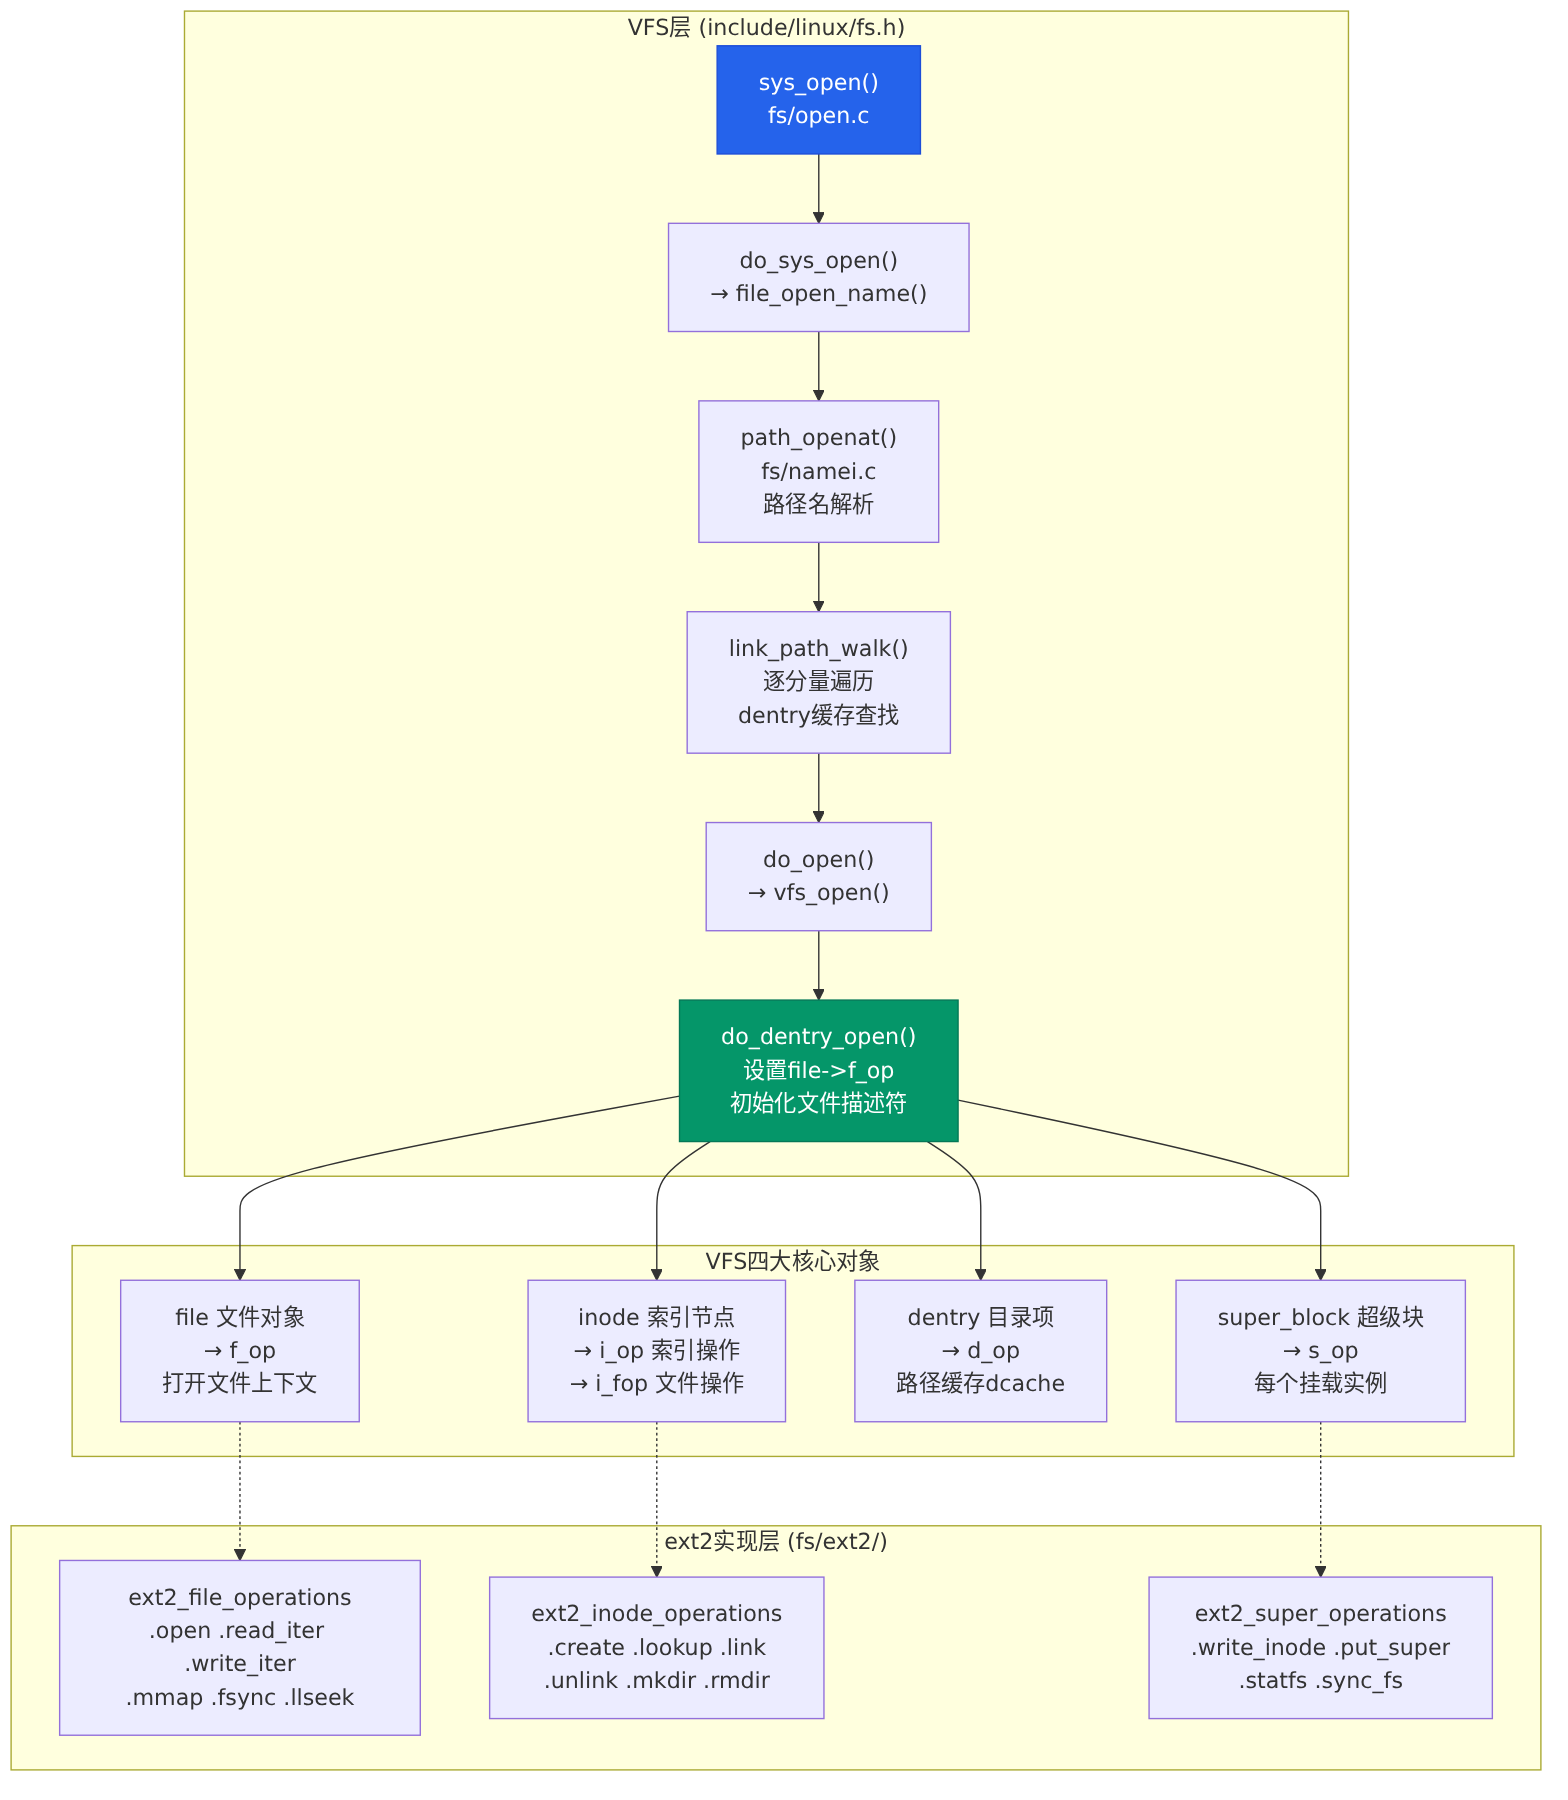
\includegraphics[width=0.95\textwidth,height=0.88\textheight,keepaspectratio]{fig_ch6_vfs_architecture.png}
\caption{VFS 核心对象模型与 ext2 实现层}
\label{fig_ch6_vfs_architecture}
\end{figure}

\subsection{路径名解析 — link\_path\_walk()}

\texttt{sys\_open() → path\_openat()}（\texttt{fs/namei.c}）是文件打开的主调用链。核心路径解析由 \texttt{link\_path\_walk()} 完成：

\begin{lstlisting}[language=C, caption={link\_path\_walk 路径解析（fs/namei.c）}, label={lst:link_path_walk}]
static int link_path_walk(const char *name, struct nameidata *nd) {
    for (;;) {
        // 1. 跳过连续的 '/'
        while (*name == '/') name++;
        // 2. 提取下一路径分量
        hash = init_name_hash(nd);
        do { hash = partial_name_hash(c, hash); } while (...);
        // 3. 在 dcache 中查找 dentry（快速路径）
        dentry = walk_component(nd, WALK_NOFOLLOW);
        // 4. 若 dcache 未命中 → 调用 i_op->lookup() 从磁盘读取
        if (IS_ERR(dentry)) break;
        // 5. 处理符号链接、挂载点穿越
        if (d_is_symlink(dentry)) { /* ... */ }
    }
}
\end{lstlisting}

\texttt{walk\_component()} 首先在 \texttt{nd->path.dentry} 的 dcache 子节点中查找（哈希 + DRCU 锁保护）。若命中（大多数情况），O(1) 返回 dentry。若未命中，调用父目录 inode 的 \texttt{i\_op->lookup()}（如 ext2 的 \texttt{ext2\_lookup()}），从磁盘读取目录项并创建新 dentry 加入 dcache。

\subsection{文件操作 — read\_iter / write\_iter}

现代 Linux 文件 I/O 通过 \texttt{read\_iter} / \texttt{write\_iter} 方法完成\cite{corbet}。这些方法接收 \texttt{struct kiocb}（内核 I/O 控制块）和 \texttt{struct iov\_iter}（用户空间缓冲区迭代器）：

\begin{lstlisting}[language=C, caption={file\_operations 结构（include/linux/fs.h）}, label={lst:fops}]
struct file_operations {
    struct module *owner;
    loff_t (*llseek)(struct file *, loff_t, int);
    ssize_t (*read)(struct file *, char __user *, size_t, loff_t *);
    ssize_t (*write)(struct file *, const char __user *, size_t, loff_t *);
    ssize_t (*read_iter)(struct kiocb *, struct iov_iter *);
    ssize_t (*write_iter)(struct kiocb *, struct iov_iter *);
    int (*mmap)(struct file *, struct vm_area_struct *);
    int (*open)(struct inode *, struct file *);
    int (*fsync)(struct file *, loff_t, loff_t, int datasync);
};
\end{lstlisting}

对于 \texttt{generic\_file\_read\_iter()}（\texttt{mm/filemap.c}），数据流为：page cache 查找 → 若未命中分配新页 → 调用 \texttt{ext2\_read\_folio()} 从磁盘填充 → \texttt{copy\_page\_to\_iter()} 复制到用户缓冲区。这是典型的"page cache → 磁盘 → 用户态"三层数据流。

\subsection{ext2 文件系统实现}

ext2 是 Linux 经典的磁盘文件系统\cite{ext2_paper,ext2_doc}。\figref{fig_ch6_ext2_structure} 展示了 ext2 的磁盘布局。

\begin{figure}[htbp]
\centering
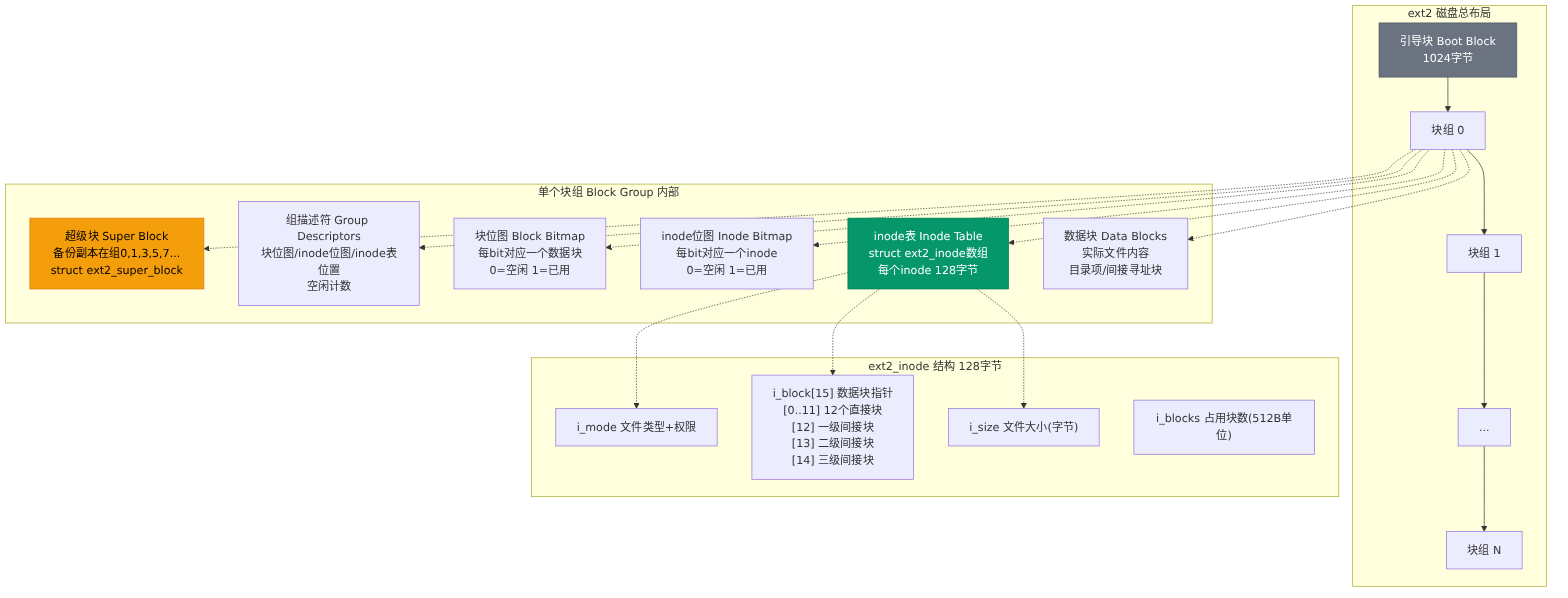
\includegraphics[width=0.95\textwidth,height=0.88\textheight,keepaspectratio]{fig_ch6_ext2_structure.png}
\caption{ext2 文件系统磁盘布局}
\label{fig_ch6_ext2_structure}
\end{figure}

\subsubsection{磁盘布局}

ext2 将磁盘划分为等大小的块组（block group），每个块组包含：Super Block（文件系统元信息，备份在特定块组中）、Group Descriptors（位图/inode 表位置）、Block Bitmap、Inode Bitmap、Inode Table、Data Blocks。

\subsubsection{ext2\_inode 与数据块寻址}

\begin{lstlisting}[language=C, caption={ext2\_inode 结构（fs/ext2/ext2.h）}, label={lst:ext2_inode}]
struct ext2_inode {
    __le16  i_mode;          // 文件类型 + 权限
    __le32  i_size;          // 文件大小（字节）
    __le32  i_blocks;        // 占用块数（512 字节单位）
    __le32  i_block[15];     // ★ 数据块指针数组
};
\end{lstlisting}

\texttt{i\_block[15]} 是 ext2 数据块寻址的核心，其设计体现了空间效率与寻址能力的经典权衡。对于小文件（≤48KB，假设 4KB 块大小），仅需 12 个直接块即可完整描述，无需间接块开销。对于中型文件，一级间接块 \texttt{i\_block[12]} 指向一个包含 \texttt{block\_size/4} 个 32 位指针的数据块（4KB 块可存 1024 个指针），额外寻址 1024 块 = 4MB 数据。二级间接 \texttt{i\_block[13]} 增加一层间接（1024×1024=1M 块 = 4GB），三级间接 \texttt{i\_block[14]} 再增一层（1024³ 块 = 4TB），足以覆盖 32 位文件偏移上限。

\texttt{ext2\_get\_block()}（\texttt{fs/ext2/inode.c}）是这一寻址机制的实现核心。给定文件的逻辑块号（文件内偏移除以块大小），该函数递归遍历间接块层级：若逻辑块号落在直接块范围（< 12），直接从 \texttt{i\_block[n]} 读取物理块号；若落在一级间接范围，先通过 \texttt{i\_block[12]} 读取一级间接块，再从中索引；以此类推。若对应物理块尚不存在（写操作导致文件扩展），则在各级间接块上分配新块，构建完整路径。

数据块分配策略受 ext2 的块分配算法影响：\texttt{ext2\_new\_block()} 在目标块组中通过块位图查找空闲块，优先选择与文件已有块物理相邻的块（减少磁盘寻道），并预留预分配块供后续扩展使用。

\subsubsection{ext2 文件操作}

ext2 的 \texttt{file\_operations} 定义于 \texttt{fs/ext2/file.c}：

\begin{lstlisting}[language=C, caption={ext2\_file\_operations 与 read\_iter/write\_iter（fs/ext2/file.c）}, label={lst:ext2_fops}]
const struct file_operations ext2_file_operations = {
    .llseek     = generic_file_llseek,
    .read_iter  = ext2_file_read_iter,
    .write_iter = ext2_file_write_iter,
    .mmap       = generic_file_mmap,
    .open       = dquot_file_open,
    .fsync      = ext2_fsync,
    .splice_read = ext2_splice_read,
};

static ssize_t ext2_file_read_iter(struct kiocb *iocb, struct iov_iter *to) {
    // 若不使用 DIO 且为缓冲 I/O，直接走 page cache 路径
    return generic_file_read_iter(iocb, to);
}
\end{lstlisting}

\texttt{generic\_file\_read\_iter()}（\texttt{mm/filemap.c}）实现缓冲 I/O 的标准数据流，是理解文件 I/O 与内存管理协同工作的关键：首先在 page cache 中查找文件偏移对应的 page（\texttt{filemap\_get\_folio()}）——若命中（大多数顺序读场景），直接通过 \texttt{copy\_page\_to\_iter()} 将内核页面的数据复制到用户空间 \texttt{iov\_iter}；若未命中（首次访问或缓存被回收），分配新 page 并调用 \texttt{filemap\_read\_folio()} → \texttt{ext2\_read\_folio()} 触发磁盘 I/O，将文件数据块读入 page cache，然后复制给用户。

\textbf{统一 Page Cache——Linux 消除双重缓存的关键设计。}经典 Unix 有一个著名的架构问题：文件数据在"buffer cache"（块设备缓存，以磁盘块为单位）和"page cache"（文件页缓存，以页为单位）中各存一份。数据从磁盘读入 buffer cache，再复制到 page cache，再复制到用户空间——两次内存拷贝、两份内存占用、一致性维护复杂。Linux 通过 \texttt{struct address\_space} 彻底解决了这一问题。

每个文件的 \texttt{inode} 拥有一个 \texttt{address\_space}（\texttt{i\_mapping}），其中的 \texttt{i\_pages}（xarray 基数树）以文件偏移量为键，映射到 page cache 中的物理页面。关键设计在于：\texttt{ext2\_file\_read\_iter()}（文件 read 路径）调用 \texttt{generic\_file\_read\_iter() → filemap\_read()} 在这个 xarray 中查找页面；\texttt{ext2\_filemap\_fault()}（文件 \texttt{mmap} 缺页路径）也在\textbf{同一个} xarray 中查找。如果 \texttt{read()} 先访问了文件偏移 0–4095，该页面进入 \texttt{address\_space}；随后 \texttt{mmap} 映射的同一文件同一偏移被访问，缺页处理在 xarray 中命中——直接映射该物理页到进程页表，无需再次读磁盘。反之亦然。

这意味着：通过 \texttt{read()} 和 \texttt{mmap()} 访问同一文件的两个进程，在物理内存中共享的是\textbf{完全相同的页面}，而不是两份独立的缓存。\texttt{open() → read() → close()} 和 \texttt{open() → mmap() → 内存访问 → munmap()} 在 page cache 层面完全统一，只是用户态接口不同。这一设计是 Linux 文件 I/O 架构的核心美学——它消除了 Unix 传承数十年的双重缓存问题，同时保证了一致性（不存在 buffer cache 已更新但 page cache 未更新的窗口）。

实验 9（ext2m 加密文件系统）的设计决策正是基于对此数据流的精确理解：XOR 加解密操作插入在 \texttt{read\_iter/write\_iter} 层而非 \texttt{read\_folio/writepages} 层，确保 page cache 始终存储密文，\texttt{read()} 和 \texttt{mmap()} 两个路径共享同样的加密语义，不会因为页缓存的一致性而产生双重加密或遗漏加密的问题。

\subsection{实验验证}

\subsubsection{实验9：ext2m 加密文件系统实现}

本实验通过复制 \texttt{fs/ext2/} 为 \texttt{fs/ext2m/} 并注册为 \texttt{"ext2m"} 新文件系统类型，实现了透明 XOR 加解密功能。核心修改位于 \texttt{fs/ext2m/file.c} 的 \texttt{ext2\_file\_read\_iter} 和 \texttt{ext2\_file\_write\_iter}。

设计关键：加密操作放置在 \texttt{read\_iter/write\_iter} 层而非更底层的 \texttt{read\_folio/writepages}。若在 \texttt{read\_folio} 中解密，readahead 预读会在 page cache 中存储解密后的明文，\texttt{read\_iter} 可能再次解密导致双重解密错误。正确做法是 page cache 始终存储密文，仅在 \texttt{generic\_file\_read\_iter()} 返回后（page cache → kernel iov）和 \texttt{copy\_to\_iter()} 前（kernel iov → userspace）之间执行解密。同理，写入时在 \texttt{copy\_from\_iter()} 后（userspace → kernel iov）和 \texttt{generic\_file\_write\_iter()} 前（kernel iov → page cache）之间执行加密。XOR 公式为 \texttt{buf[i] \^{}= key[(i + block*7) \% 16]}，其中 block = pos >> PAGE\_SHIFT，使得同一文件的不同块使用不同的密钥偏移。

验证方法展示了分层理解：创建 100MB ext2 磁盘镜像（\texttt{dd + mkfs.ext2}），以 \texttt{-t ext2m} 挂载后 echo 写入明文、cat 读取明文——加解密对用户透明；以 \texttt{-t ext2} 重新挂载同一镜像，\texttt{xxd} 查看磁盘原始字节为密文，且首字节 \texttt{0x07} = \texttt{0x48('H') \^{} 0x4F(key[0])} 通过数学验算证实 XOR 运算正确。同一磁盘镜像可在 ext2 和 ext2m 之间交叉挂载而无数据丢失，证实 ext2m 的磁盘格式与 ext2 完全兼容（仅运行时加解密）。该实验完整验证了 VFS 层 \texttt{file\_operations} 覆盖、page cache 数据流、ext2 磁盘布局以及文件系统类型注册的全链路。

\subsubsection{实验7：Linux 设备文件与驱动程序}

本实验编写了两个内核模块，验证了 VFS 的 \texttt{file\_operations} 在字符设备上的应用。

\texttt{hello\_module} 作为内核模块的最小骨架，通过 \texttt{module\_init/exit} 注册加载和卸载回调，\texttt{printk} 输出验证模块生命周期。

\texttt{char\_driver} 实现完整的字符设备驱动。设备注册链路：\texttt{alloc\_chrdev\_region()} 动态分配主设备号（避免了静态指定可能的冲突）→ \texttt{cdev\_init(\&my\_cdev, \&fops)} 将 \texttt{file\_operations} 绑定到 cdev → \texttt{cdev\_add()} 注册到内核 → \texttt{class\_create() + device\_create()} 触发 udev 自动创建 \texttt{/dev/mychardev} 设备节点（主设备号 242，动态分配）。\texttt{file\_operations} 实现了七个回调：\texttt{.open}（引用计数递增）、\texttt{.read}（通过 \texttt{for\_each\_process(task)} 遍历全部内核进程，使用 \texttt{rcu\_read\_lock/rcu\_read\_unlock} 保护，\texttt{scnprintf} 格式化 PID/状态/优先级/PPID/进程名，\texttt{copy\_to\_user} 输出到用户空间）、\texttt{.write}（从用户空间接收数据）、\texttt{.unlocked\_ioctl}（设备控制命令）、\texttt{.release}（引用计数递减）。卸载时按创建逆序释放（\texttt{device\_destroy → class\_destroy → cdev\_del → unregister\_chrdev\_region}），防止资源泄漏。

验证过程：\texttt{insmod} 加载后 \texttt{ls -la /dev/mychardev} 显示 \texttt{c rw------- 1 root root 242, 0}；用户态测试程序依次执行 open/write/read/ioctl/close 全链路，read 返回的进程列表包含所有用户进程和内核线程。\texttt{rmmod} 后设备文件自动消失。该实验验证了 VFS 层 \texttt{file\_operations} 的统一接口设计——ext2 文件的 \texttt{read\_iter} 和字符设备的 \texttt{.read} 均通过 \texttt{struct file\_operations} 回调提供服务，上层 \texttt{read()} 系统调用对二者无差别。

%========================================== 总结 ==========================================
\section{总结} \label{sec:conclusion}

本报告以 Linux 6.18.15 内核源码为分析对象，对操作系统内核的核心子系统进行了系统性的源码阅读与分析。

\textbf{进程管理方面}：深入分析了 \texttt{task\_struct} 进程描述符的结构设计、六态进程状态机的变迁规则、\texttt{kernel\_clone() → copy\_process()} 的进程创建全流程（dup\_task\_struct → sched\_fork → copy\_mm → copy\_thread → wake\_up\_new\_task），以及系统调用从用户态 \texttt{syscall} 指令到 \texttt{do\_syscall\_64()} 分发的完整路径。

\textbf{进程调度方面}（本报告重点）：完整剖析了从 \texttt{schedule() → \_\_schedule() → pick\_next\_task() → context\_switch() → switch\_to → \_\_switch\_to\_asm → \_\_switch\_to()} 的七层调用链。对 CFS/EEVDF 公平调度算法（\texttt{\_\_pick\_eevdf()} 红黑树选择逻辑、entity\_tick 时钟抢占、enqueue/dequeue 入队出队）、RT/DL 实时调度以及 x86\_64 架构下 RSP 切换点、callee-saved 寄存器保存/恢复、CR3 地址空间切换（PCID/ASID）、FPU/FS/GS 架构收尾进行了逐寄存器级的详细分析。

\textbf{进程间通信方面}：分析了 System V IPC 三件套（信号量 \texttt{semop} 原子操作、消息队列、共享内存零拷贝）的内核实现、信号的 send→pending→handle→sigreturn 全生命周期、管道环形缓冲区机制。

\textbf{内存管理方面}：分析了伙伴系统（\texttt{free\_area[order]} 分配/释放/分裂/合并）、slub 分配器、VMA 与 mmap 惰性分配、缺页异常四种处理路径（anonymous/swap/file/COW）、\texttt{do\_wp\_page()} 的引用计数优化以及 kswapd 页面回收与换出机制。

\textbf{文件系统方面}：分析了 VFS 四对象模型（super\_block/inode/dentry/file）、\texttt{link\_path\_walk()} 路径名解析（dcache 快速路径 + \texttt{i\_op->lookup()} 慢速路径）、ext2 磁盘布局（块组/super block/inode table/\texttt{i\_block[15]} 间接块寻址）以及 \texttt{read\_iter/write\_iter} 的 page cache 数据流。

\subsection{跨子系统设计模式}

分别阅读六个子系统后可以识别出一些反复出现的设计模式。这些模式不是某个文件或函数的局部选择，而是 Linux 内核在演化中收敛形成的"设计语言"，理解它们有助于在阅读任何内核代码时更快地建立心智模型：

\begin{table}[htbp]
\centering
\footnotesize
\caption{Linux 内核跨子系统设计模式}
\label{tab:design_patterns}
\begin{tabular}{p{2cm}p{3cm}p{3cm}p{3cm}p{2.5cm}}
\toprule
\textbf{模式} & \textbf{调度器} & \textbf{内存管理} & \textbf{文件系统/VFS} & \textbf{IPC} \\
\midrule
\textbf{惰性求值} & 新进程不分配时间片直到被 \texttt{pick\_task} 选中；MFQ 的 \texttt{mfq\_entity\_init} 在首次 \texttt{enqueue} 时才调用 & COW 延迟物理页复制；缺页异常按需分配页框；VMA 惰性映射（\texttt{mmap} 只建 VMA 不分配页） & dentry 按需创建（\texttt{lookup} 慢路径）；inode 延迟从磁盘读取 & 共享内存惰性附加（\texttt{shmat} 只建 VMA，首次访问才在 \texttt{shmem\_fault} 中映射物理页）\\
\midrule
\textbf{快慢路径分离} & \texttt{pick\_next\_task} 快速路径：全 CFS 任务时直接走 \texttt{fair}；慢速路径：\texttt{for\_each\_active\_class} 遍历全部调度类 & \texttt{get\_page\_from\_freelist} 快速路径：伙伴系统直接分配；慢速路径：\texttt{\_\_alloc\_pages\_slowpath} → 压缩→回收→OOM & \texttt{walk\_component} 快速路径：dcache 哈希命中 O(1)；慢速路径：\texttt{i\_op->lookup()} 磁盘 I/O & futex 快速路径：用户态 CAS 无竞争直接返回；慢速路径：\texttt{futex(FUTEX\_WAIT)} 进内核睡眠 \\
\midrule
\textbf{RCU + 引用计数} & \texttt{rq->curr} 用 RCU 保护读取，\texttt{task\_struct} 的 \texttt{usage} 引用计数控制释放 & \texttt{folio\_ref\_count} 保护页面生命周期；\texttt{mm\_struct} 的 \texttt{mm\_users/mm\_count} 双重计数 & dentry 的 \texttt{d\_lockref}（混合 spinlock + 引用计数）；inode 的 \texttt{i\_count} & \texttt{sem\_array→sem\_perm.refcount}；共享内存 \texttt{shmid\_kernel} 的引用计数 \\
\midrule
\textbf{per-CPU 隔离} & \texttt{struct rq} per-CPU；MFQ 的 \texttt{DEFINE\_PER\_CPU(mfq\_rq)}；调度类无需全局锁 & per-CPU page cache（\texttt{struct per\_cpu\_pages}）；slub 的 per-CPU  slab 缓存 & — & — \\
\midrule
\textbf{分裂返回} & \texttt{schedule()} 在 \texttt{context\_switch} 后返回时可能在另一个进程中 & \texttt{fork()} 父子同时返回但返回值不同（子=0，父=pid） & — & \texttt{semop()} 阻塞睡眠后返回：内核在 \texttt{perform\_atomic\_semop} 失败后 \texttt{schedule\_timeout}，进程被 V 操作唤醒后"看起来"从 \texttt{semop()} 调用处继续 \\
\bottomrule
\end{tabular}
\end{table}

这五种模式贯穿了从进程管理到文件系统的全部六个子系统。"惰性求值"最小化初始开销（fork 廉价 + COW 减拷贝 + dcache 减磁盘 I/O），"快慢路径分离"保证常见情况零开销（全 CFS 不走遍历 + dcache 命中不走磁盘 + futex 无竞争不陷入内核），"RCU + 引用计数"在性能和安全性之间取得平衡（读端免锁 + 生命周期精确控制），"per-CPU 隔离"消除全局锁竞争（每个 CPU 独立运行队列和页缓存），"分裂返回"将异步语义包装为同步调用接口（fork 一个调用两个返回 + schedule 睡眠透明）。

每章末尾附带的课程实验验证（共 11 个）从实践层面印证了源码分析的理论认知。这些实验不仅覆盖了内核各子系统的基本操作，更关键的是——实验 4 的 XSI 信号量、实验 8 的内核死锁检测、实验 11 的 MFQ 调度器实现——直接触及了内核源码的修改和扩展，将"阅读"上升到了"理解和操作"的层次。

%========================================== 参考文献 ==========================================
\begin{thebibliography}{99}

% 内核源码与文档
\bibitem{lkml} Linux Kernel Community. Linux 6.18.15 kernel source tree[EB/OL]. \texttt{https://git.kernel.org/pub/scm/linux/kernel/git/stable/linux.git}, 2025.

\bibitem{sched_cfs} Linux Kernel Documentation. CFS Scheduler Design[EB/OL]. \texttt{Documentation/scheduler/sched-design-CFS.rst}.

\bibitem{sched_eevdf} Linux Kernel Documentation. EEVDF Scheduler[EB/OL]. \texttt{Documentation/scheduler/sched-eevdf.rst}.

\bibitem{sched_dl} Linux Kernel Documentation. Deadline Task Scheduling[EB/OL]. \texttt{Documentation/scheduler/sched-deadline.rst}.

\bibitem{mm_doc} Linux Kernel Documentation. Memory Management[EB/OL]. \texttt{Documentation/admin-guide/mm/}, \texttt{Documentation/mm/}.

\bibitem{vfs_doc} Linux Kernel Documentation. Overview of the Linux Virtual File System[EB/OL]. \texttt{Documentation/filesystems/vfs.rst}.

\bibitem{ext2_doc} Linux Kernel. ext2 文件系统数据结构定义[EB/OL]. \texttt{fs/ext2/ext2.h}, Linux 6.18.15.

% 经典教材
\bibitem{love} Robert Love. Linux Kernel Development (3rd Edition)[M]. Addison-Wesley Professional, 2010.

\bibitem{bovet} Daniel P. Bovet, Marco Cesati. Understanding the Linux Kernel (3rd Edition)[M]. O'Reilly Media, 2005.

\bibitem{corbet} Jonathan Corbet, Alessandro Rubini, Greg Kroah-Hartman. Linux Device Drivers (3rd Edition)[M]. O'Reilly Media, 2005.

\bibitem{tanenbaum} Andrew S. Tanenbaum, Herbert Bos. Modern Operating Systems (4th Edition)[M]. Pearson, 2014.

\bibitem{gorman} Mel Gorman. Understanding the Linux Virtual Memory Manager[M]. Prentice Hall, 2004.

\bibitem{mckenney} Paul E. McKenney. Is Parallel Programming Hard, And, If So, What Can You Do About It?[M]. kernel.org, 2023.

\bibitem{maurice} Maurice J. Bach. The Design of the UNIX Operating System[M]. Prentice-Hall, 1986.

\bibitem{stevens} W. Richard Stevens, Stephen A. Rago. Advanced Programming in the UNIX Environment (3rd Edition)[M]. Addison-Wesley, 2013.

\bibitem{silberschatz} Abraham Silberschatz, Peter B. Galvin, Greg Gagne. Operating System Concepts (10th Edition)[M]. Wiley, 2018.

% x86 架构手册
\bibitem{intel_sdm} Intel Corporation. Intel 64 and IA-32 Architectures Software Developer's Manual, Volume 3A: System Programming Guide[EB/OL]. 2025.

\bibitem{amd_apm} AMD Corporation. AMD64 Architecture Programmer's Manual, Volume 2: System Programming[EB/OL]. 2024.

\bibitem{x86_abi} System V Application Binary Interface: AMD64 Architecture Processor Supplement[S]. 2023.

% LWN 技术文章
\bibitem{lwn_cfs} Jonathan Corbet. CFS scheduler overview[EB/OL]. LWN.net, \texttt{https://lwn.net/Articles/230574/}, 2007.

\bibitem{lwn_eevdf} Jonathan Corbet. The EEVDF scheduler[EB/OL]. LWN.net, \texttt{https://lwn.net/Articles/925371/}, 2023.

\bibitem{lwn_rcu} Paul E. McKenney. What is RCU?[EB/OL]. LWN.net, \texttt{https://lwn.net/Articles/262464/}, 2007.

\bibitem{lwn_mm} Jonathan Corbet. Memory management documentation index[EB/OL]. LWN.net, \texttt{https://lwn.net/Kernel/Index/}, 2004–2025.

\bibitem{lwn_context_switch} Jonathan Corbet. A deep dive into context switching[EB/OL]. LWN.net, \texttt{https://lwn.net/Articles/542893/}, 2013.

\bibitem{lwn_page_fault} Jonathan Corbet. Page fault handling in the Linux kernel[EB/OL]. LWN.net, \texttt{https://lwn.net/Articles/546612/}, 2013.

% 内核子系统论文
\bibitem{eevdf_paper} Peter Zijlstra. Earliest Eligible Virtual Deadline First: A Flexible and Accurate Scheduling Policy[C]. Linux Plumbers Conference, 2023.

\bibitem{cfs_paper} Ingo Molnár. Modular Scheduler Core and Completely Fair Scheduler[C]. Linux Kernel Summit, 2007.

\bibitem{mfq_paper} Fernando J. Corbató, et al. An Experimental Time-Sharing System[C]//Proc. of the Spring Joint Computer Conference. ACM, 1962: 335-344.

\bibitem{ext2_paper} Rémy Card, Theodore Ts'o, Stephen Tweedie. Design and Implementation of the Second Extended Filesystem[C]//Proc. of the First Dutch International Symposium on Linux. 1995.

\bibitem{stallings} William Stallings. Operating Systems: Internals and Design Principles (9th Edition)[M]. Pearson, 2017.

\end{thebibliography}

\end{document}
